%
% Template Laporan Tugas Akhir Jurusan Informatika Unsyiah 
%
% @author  Kurnia Saputra 
% @version 1.0
% @since 03.02.2016
%
% Template ini telah disesuaikan dengan aturan penulisan tugas akhir yang terdapat pada dokumen Panduan Tugas Akhir FMIPA Unsyiah tahun 2016.
%


% Template pembuatan naskah tugas akhir.
\documentclass{jifhasil-sidang}

\tolerance=1
\emergencystretch=\maxdimen
\hyphenpenalty=10000
\hbadness=10000

%\usepackage[a4paper,left=14cm,right=3cm,top=3cm,bottom=5cm]{geometry}

% Daftar pemenggalan suku kata dan istilah dalam LaTeX
%
% Hyphenation untuk Indonesia 
%
% @author  Andreas Febrian
% @version 1.00
% 
% Tambahkan cara pemenggalan kata-kata yang salah dipenggal secara otomatis 
% oleh LaTeX. Jika kata tersebut dapat dipenggal dengan benar, maka tidak 
% perlu ditambahkan dalam berkas ini. Tanda pemenggalan kata menggunakan 
% tanda '-'; contoh:
% menarik
%   --> pemenggalan: me-na-rik
%

\hyphenation{
    % alphabhet A
    a-na-li-sa a-tur 
    a-pli-ka-si 
    android
    % alphabhet B
    ba-ngun-an 
    be-be-ra-pa 
    ber-ge-rak
    ber-ke-lan-jut-an 
    ber-pe-nga-ruh 
    % alphabhet C
    ca-ri
    % alphabhet D
    di-sim-pan di-pim-pin de-ngan da-e-rah di-ba-ngun da-pat di-nya-ta-kan 
    di-sim-bol-kan di-pi-lih di-li-hat de-fi-ni-si
    % alphabhet E
    e-ner-gi eks-klu-sif
    % alphabhet F
    fa-si-li-tas
    foot-print
    % alphabhet G
    ga-bung-an ge-rak
    % alphabhet H
    ha-lang-an
    % alphabhet I
    % alphabhet J
    % alphabhet K
    ke-hi-lang-an
    ku-ning 
    kua-li-tas ka-me-ra ke-mung-kin-an ke-se-pa-ham-an
    % alphabhet L
    ling-kung-an
    % alphabhet M
    me-neng-ah
    meng-a-tas-i me-mung-kin-kan me-nge-na-i me-ngi-rim-kan 
    meng-u-bah meng-a-dap-ta-si me-nya-ta-kan mo-di-fi-ka-si
    meng-a-tur
    mem-pro-mo-si-kan
    me-la-ku-kan
    meng-i-den-ti-fi-ka-si-kan
    % alphabhet N
    nya-ta non-eks-klu-sif
    % alphabhet O
    % alphabhet P
	pe-nye-rap-an 
	pe-ngon-trol
    pe-mo-del-an
    pe-ran  pe-ran-an-nya
    pem-ba-ngun-an pre-si-den pe-me-rin-tah prio-ri-tas peng-am-bil-an 
    peng-ga-bung-an pe-nga-was-an pe-ngem-bang-an 
    pe-nga-ruh pa-ra-lel-is-me per-hi-tung-an per-ma-sa-lah-an 
    pen-ca-ri-an peng-struk-tur-an
    pe-ran-ca-ngan
    plat-form
    patch
    % alphabhet Q
    % alphabhet R
    ran-cang-an
    % alphabhet S
    si-mu-la-si sa-ngat
    smart-phone
    % alphabhet T
    te-ngah
    ter-da-pat
    % alphabhet U
    % alphabhet V
    % alphabhet W
    % alphabhet X
    % alphabhet Y
    % alphabhet Z
    % special
}

% Untuk prefiks pada daftar gambar dan tabel
\usepackage[titles]{tocloft}
\renewcommand\cftfigpresnum{Gambar\  }
\renewcommand\cfttabpresnum{Tabel\   }

\newcommand{\listappendicesname}{DAFTAR LAMPIRAN}
\newlistof{appendices}{apc}{\listappendicesname}
\newcommand{\appendices}[1]{\addcontentsline{apc}{appendices}{#1}}
\newcommand{\newappendix}[1]{\section*{#1}\appendices{#1}}

% Untuk hyperlink dan table of content
\usepackage[hidelinks]{hyperref}
\renewcommand\UrlFont{\rmfamily\itshape} %it's me!
\newlength{\mylenf}
\settowidth{\mylenf}{\cftfigpresnum}
\setlength{\cftfignumwidth}{\dimexpr\mylenf+2em}
\setlength{\cfttabnumwidth}{\dimexpr\mylenf+2em}

% Agar ada tulisan BAB pada TOC
\renewcommand\cftchappresnum{BAB } 
  \cftsetindents{chapter}{0em}{4.5em} %indenting bab
  \cftsetindents{section}{4.5em}{2em}
  \cftsetindents{subsection}{6.5em}{3em}
 
% Agar di TOC setiap angka bab/subbab diakhiri titik

\renewcommand{\cftsecaftersnum}{.}
\renewcommand{\cftsubsecaftersnum}{.}

% Agar setiap angka bab/subbab diakhiri titik
\usepackage{titlesec}
\titlelabel{\thetitle.\quad}

% Agar disetiap caption table dan gambar diakhiri titik
\usepackage[labelsep=period]{caption}

% Untuk Bold Face pada Keterangan Gambar
\usepackage[labelfont=bf]{caption}

% Untuk caption dan subcaption
\usepackage{caption}
\usepackage{subcaption}


% Agar bisa menggunakan warna LaTeX
\usepackage{color} %it's me!

% Agar table yang panjang bisa cut ke next page    %byRennyAdr
\usepackage{longtable}

% Untuk page landscape        %byRennyAdr
\usepackage{pdflscape}
\usepackage{lscape}

% Agar bisa bikin code snippet
\usepackage{listings, lstautogobble} %it's me!

% untuk shadow gambar     %tomy
\usepackage{fancybox, graphicx}


% Warna pada code snippet Java
\definecolor{javared}{rgb}{0.6,0,0} % untuk strings
\definecolor{javagreen}{rgb}{0.25,0.5,0.35} % untuk comments
\definecolor{javapurple}{rgb}{0.5,0,0.35} % untuk keywords
\definecolor{javadocblue}{rgb}{0.25,0.35,0.75} % untuk javadoc

% Warna pada code snippet C/C++
\definecolor{mygray}{rgb}{0.4,0.4,0.4}
\definecolor{mygreen}{rgb}{0,0.8,0.6}
\definecolor{myorange}{rgb}{1.0,0.4,0}

% menambah keyword pada Android XML - tomy
\lstdefinelanguage[Android]{XML}[]{XML} {
	morekeywords={
		android:background,
		android:clickable,
		android:contentDescription,
		android:iconifiedByDefault,
		android:id,
		android:layout_alignParentBottom,
		android:layout_alignParentRight,
		android:layout_height,
		android:layout_marginBottom,
		android:layout_marginLeft,
		android:layout_marginRight,
		android:layout_marginStart,
		android:layout_weight,
		android:layout_width,
		android:layout_below,
		android:listSelector,
		android:orientation,
		android:paddingLeft,
		android:scaleType,
		android:src,
		android:text,
		android:textAppearance,
		android:textSize,
		android:textStyle,
		tools:context,
		xmlns:android,
		xmlns:tools,
		xmlns:app,
		android:layout_marginTop,
		android:layout_centerHorizontal,
		android:layout_centerVertical,
		android:drawableLeft,
		android:drawablePadding,
		android:hint,
		android:textColor,
		android:inputType,		
	}     
}

% warna code snippet Android XML - tomy
\definecolor{AndroidXMLIdentifierstyle}{HTML}{ffba00}
\definecolor{AndroidXMLComment}{HTML}{645FCA}
\definecolor{AndroidXMLString}{HTML}{228b22}
\definecolor{AndroidXMLKeyword}{HTML}{7F007F}

% warna code snippet PHP
\definecolor{backcolor}{rgb}{0.95,0.95,0.96}

\lstset{
	language=php,
	backgroundcolor=\color{backcolor},
	commentstyle=\color{mygreen},
	keywordstyle=\color{javadocblue},
	stringstyle=\color{javared},
	basicstyle=\ttfamily\footnotesize,
	numbers=left,
	% breakatwhitespace=false,
	breaklines=true,
	% keepspaces=true,
	% numbersep=5pt,
	% showspaces=false,
	% showtabs=false,
	tabsize=4,
	numberstyle=\footnotesize,
	% xleftmargin=10pt,
	emph            =[1]{return, public, function},
	emphstyle       =[1]\color{javadocblue},
	% showstringspaces=false,
	captionpos=b,
}

% Sampul Depan
%-----------------------------------------------------------------
% Sampul Depan
%-----------------------------------------------------------------
\judul{RANCANG BANGUN APLIKASI PENJUALAN TANAMAN HIDROPONIK BERBASIS WEB (STUDI KASUS : KELOMPOK PENJUAL HIDROPONIK BANDA ACEH)
}

% \judulinggris{\textit{}}

% nama lengkap
\fullname{Muhammad Kautsar}

% NPM (Nomor Pokok Mahasiswa)
\idnum{1608107010020}

\degree{Sarjana Komputer}

\yearsubmit{September, 2021}

\program{Informatika}

\dept{Informatika}

% Pembimbing Pertama
\firstsupervisor{Kurnia Saputra, S.T., M.Sc.}
\firstnip{198003262014041001}

% Pembimbing Kedua
\secondsupervisor{Viska Mutiawani, B.IT, M.IT.}
\secondnip{198008312009122003}

% Ketua Jurusan
\kajur{Dr. Muhammad Subianto, S.Si., M.Si}
\kajurnip{196812111994031005}

% Dekan Fakultas
%\dekan{Dr. Teuku Mohamad Iqbalsyah, S.Si., M.Sc.}
%\dekannip{197110101997031003}

% tangal lulus proposal, seminar hasil atau sidang
\approvaldate{                               }

%-----------------------------------------------------------------
% End of Sampul Depan
%-----------------------------------------------------------------


% Awal dokumen
\usepackage{fancyhdr}
\usepackage{rotating}
% Untuk prefiks pada Daftar Program   
% byRennyAdr
\makeatletter
\begingroup\let\newcounter\@gobble\let\setcounter\@gobbletwo
\globaldefs\@ne \let\c@loldepth\@ne
\newlistof{listings}{lol}{\lstlistlistingname}
\endgroup
\let\l@lstlisting\l@listings
\AtBeginDocument{\addtocontents{lol}{\protect\addvspace{10\p@}}}
\makeatother
\renewcommand{\lstlistoflistings}{\listoflistings}
\renewcommand\cftlistingspresnum{Program~}
\cftsetindents{listings}{1.5em}{7em}

%tab didaftar pustaka -Indah
\setlength{\bibhang}{30pt}

%split rumus -Indah
\usepackage{amsmath}

\begin{document}
\fancyhf{} 
\fancyfoot[C]{\thepage}


\cover

\approvalpage

%-----------------------------------------------------------------
% Disini kata pengantar
%-----------------------------------------------------------------
\begin{abstractind}

Perkembangan teknologi informasi yang pesat telah memberikan banyak manfaat dalam berbagai aspek kehidupan, tak terkecuali dibidang UMKM. Dimana para pelaku UMKM saat ini telah memanfaatkan teknologi informasi dalam memasarkan produknya secara digital, diantaranya menggunakan aplikasi media sosial. Hal inilah yang dilakukan oleh para kelompok UMKM tanaman hidroponik yang ada di kota Banda Aceh, hanya saja cara ini dinilai masih memiliki beberapa kekurangan yaitu diantaranya akses yang terbatas antara calon pembeli dengan penjual dikarenakan tidak semua calon pembeli mengetahui akun media sosial penjual dan juga pembeli tidak dapat mengetahui dengan pasti ketersediaan produk yang ditawarkan oleh penjual. Oleh karena itu, pada penelitian ini menawarkan solusi atas permasalahan tersebut berupa aplikasi berbasis web yang dapat membantu UMKM hidroponik untuk memasarkan produknya dengan lebih mudah dan efesien. Pada aplikasi ini terdapat 2 tipe \textit{user} yaitu admin dan penjual. Dimana admin dapat menggunakan aplikasi untutk mengelola data dan mendaftarkan akun penjual, sedangkan penjual dapat menggunakan aplikasi ini untuk menjual produknya dan menerima pesanan dari pembeli. Proses rancang bangun aplikasi dimulai dari tahap analisis kebutuhan, perancangan sistem, kemudian dilanjutkan dengan pembuatan aplikasi dan pengujian aplikasi. Pembuatan aplikasi penjualan berbasis web ini dibangun menggunakan \textit{framework} Laravel dan MySQL sebagai \textit{database}. Pada aplikasi ini juga dibuatkan REST API untuk digunakan sebagai \textit{backend} pada aplikasi berbasis Android. Setelah aplikasi selesai dibuat, dilakukan pengujian fungsionalitas menggunakan metode \textit{Black Box} dan pengujian \textit{usability} menggunakan \textit{Usability Metric for User Experience} (UMUX). Pengujian fungsionalitas menghasilkan nilai yang 'sesuai' dan begitu pula hasil dari pengujian UMUX menghasilkan nilai 86.66\% dari kepuasan pengguna.


\bigskip
\noindent
\textbf{Kata kunci :} UMKM, Hidroponik, web, Laravel, \textit{framework}, MySQL, \textit{Black Box, Usability Metric for User Experience.}
\end{abstractind} %berikan comment jika proposal

\begin{abstracteng}
\textit{Hydroponic MSME actors in Banda Aceh have used social media applications to market their products. But unfortunately this method still has drawbacks such as limited access, potential buyers not knowing the seller's social media accounts and also the availability of hydroponic vegetables which are difficult to detect. Therefore, this study offers a solution to these problems in the form of a web-based application that can help hydroponic SMEs to market their products more easily and efficiently. In this application there are 3 types of users, namely superadmin, admin and seller. Superadmin and admin users can use the application to manage data, but there is a difference where superadmin is in charge of registering an admin account while the admin is in charge of registering a seller's account, then sellers can use this application to sell their products and receive orders from buyers. The application design process starts from the requirements analysis stage, system design, then continues with application creation and application testing. Making a web-based sales application is built using the Laravel framework and MySQL as a place to store the database. In this application, a REST API is also made to be used as a backend for Android-based applications. After the application is completed, functional testing is carried out using the Black Box method and usability testing using the Usability Metric for User Experience (UMUX). Functionality testing returns 'fit' values for all tested functions. While the results of usability testing produce a value of 82.12 from user satisfaction.}

\bigskip
\noindent
\textbf{\emph{Keywords :}} \textit{MSME, Hydroponic, Laravel, MySQL, Black Box, Usability Metric for User Experience.}
\end{abstracteng} %berikan comment jika proposal

\preface % Note: \preface JANGAN DIHAPUS!


Segala puji dan syukur atas ke hadirat Allah SWT yang telah melimpahkan rahmat dan karunia-Nya kepada kita semua, sehingga penulis dapat menyelesaikan penulisan tugas akhir ini yang berjudul \textbf{“Rancang Bangun Aplikasi Penjualan Tanaman Hidroponik Berbasis Web (Studi Kasus : Kelompok Penjual Hidroponik Banda Aceh)”}. Penulis menyadari penulisan tugas akhir ini tidak terlepas dari dukungan, pengarahan, bimbingan, dan bantuan dari berbagai pihak. Oleh karena itu, melalui tulisan ini penulis mengucapkan rasa terima kasih kepada:

\begin{enumerate}
	\item{Ayah dan Ibu sebagai kedua orang tua penulis yang senantiasa selalu mendukung aktivitas dan kegiatan yang penulis lakukan baik secara moral maupun material serta menjadi motivasi terbesar bagi penulis untuk menyelesaikan Tugas Akhir ini.}
	\item{Bapak Kurnia Saputra, M.Sc., selaku Dosen Pembimbing I dan Ibu Viska Mutiawani, B.IT, M.IT., selaku Dosen Pembimbing II yang telah banyak memberikan bimbingan dan arahan kepada penulis, sehingga penulis dapat menyelesaikan Tugas akhir ini.}
	\item {Ibu Viska Mutiawani, B.IT, M.IT., selaku Ketua Jurusan Informatika.}
	\item{Bapak Zahnur S.Si, M.Info Tech., selaku Dosen Wali.}
	\item{Seluruh Dosen di Jurusan Informatika Fakultas MIPA atas ilmu dan didikannya selama perkuliahan.}
	\item{Sahabat dan teman-teman seperjuangan Jurusan Informatika Unsyiah 2016 lainnya.}
\end{enumerate}

% \vspace{6cm}

Penulis juga menyadari segala yang terdapat di dalamnya jauh dari kata sempurna baik dari segi materi, cara, ataupun bahasa yang disajikan. Seiring dengan ini penulis mengharapkan kritik dan saran dari pembaca yang sifatnya dapat berguna untuk kesempurnaan Tugas Akhir ini. Harapan penulis semoga tulisan ini dapat bermanfaat bagi banyak pihak dan untuk perkembangan ilmu pengetahuan.

\vspace{1cm}


\begin{tabular}{p{7.5cm}c}
	&Banda Aceh, Desember 2021\\
	&\\
	&\\
	&\\
	&\textbf{Penulis}
\end{tabular}



%-----------------------------------------------------------------
% TOC menggunakan single space
%-----------------------------------------------------------------

\begin{singlespace}
	\tableofcontents
\end{singlespace}

\addcontentsline{toc}{chapter}{DAFTAR ISI}
\listoftables
\addcontentsline{toc}{chapter}{DAFTAR TABEL}
\listoffigures
\addcontentsline{toc}{chapter}{DAFTAR GAMBAR}

\renewcommand{\lstlistlistingname}{DAFTAR PROGRAM}
\lstlistoflistings
\addcontentsline{toc}{chapter}{DAFTAR PROGRAM}

\listofappendices
\addcontentsline{toc}{chapter}{DAFTAR LAMPIRAN}

%-----------------------------------------------------------------
% Daftar Singkatan 
%-----------------------------------------------------------------
\include{daftar-singkatan}

% Caption untuk code snippet. it's me!
\renewcommand{\thelstlisting}{\arabic{chapter}.\arabic{lstlisting}}
\renewcommand*\lstlistingname{Program}

%-----------------------------------------------------------------
% Disini awal masukan untuk Bab
%-----------------------------------------------------------------
\begin{onehalfspace}

\fancyhf{} 
\fancyfoot[C]{\thepage}
\pagenumbering{arabic}


\fancyhf{} 
\fancyfoot[C]{\thepage}

\chapter{PENDAHULUAN}

\section{\uppercase{LATAR BELAKANG}}
UMKM (Usaha Mikro Kecil Menengah) adalah unit usaha produktif yang berdiri sendiri, yang dilakukan oleh orang perorangan atau Badan usaha di semua sektor ekonomi \citep{tambunan2012peluang}. UMKM sering disebut sebagai salah satu pilar kekuatan perekonomian suatu daerah. Hal ini disebabkan karena UMKM mempunyai fleksibilitas dan kemampuan menyesuaikan diri terhadap kondisi pasar yang berubah dengan cepat dibanding dengan perusahaan skala besar \citep{sartika2002ekonomi}. Hal itulah yang membuat UMKM dapat bertahan walaupun dalam kondisi pandemi seperti sekarang ini.

\par Perkembangan teknologi yang sangat pesat di era globalisasi saat ini telah memberikan banyak manfaat dalam berbagai aspek kehidupan, termasuk dibidang UMKM. Dimana para pelaku UMKM sekarang ini dapat memanfaatkan kemajuan teknologi tersebut untuk memasarkan produknya secara digital. Pemasaran digital adalah pemasaran yang memanfaatkan akses internet, media sosial, maupun perangkat digital lainnya \citep{hardilawati2020strategi}. Dengan melakukan pemasaran secara digital dapat menjangkau pelanggan yang lebih luas lagi dan mempromosikan produk-produk kepada calon pembeli baru. Melihat banyaknya keuntungan dari pemasaran secara digital membuat para pelaku usaha tanaman hidroponik yang ada di Banda Aceh pun tertarik untuk memasarkan produknya secara digital.

\par Hidroponik adalah sistem penanaman tanaman tanpa menggunakan media tanam tanah dan menggunakan larutan nutrisi yang mengandung garam organik untuk menumbuhkan perakaran yang ideal \citep{rosliani2005budidaya}. Pelaku UMKM hidroponik ini, sebenarnya sudah memasarkan produknya secara digital lewat aplikasi sosial media seperti WhatsApp dan Instagram, hanya saja penjualannya dinilai masih kurang efektif karena pelanggannya hanya berasal dari orang yang mengetahui kontak dan sosial media mereka saja, belum lagi mengenai ketersediaan produknya yang harus ditanyakan terlebih dahulu kepada penjualnya. Berangkat dari permasalahan tersebut pihak UMKM hidroponik berencana untuk memasarkan produknya lewat aplikasi khusus yang bertindak sebagai \textit{e-commerce} agar mempermudah proses transaksi antara penjual dan pembeli, juga diharapkan dapat meningkatkan angka penjualannya.

\par Berdasarkan uraian diatas, penulis di sini bertugas untuk merancang dan membangun sebuah aplikasi berbasis web untuk admin dan penjual. Aplikasi ini nantinya akan diintegrasikan dengan aplikasi berbasis android untuk melakukan pembelian produk tanaman hidroponik. Pembuatan aplikasi penjualan berbasis web ini dibangun menggunakan \textit{framework} Laravel dan MySQL sebagai \textit{database}. Selain itu, juga akan dibuatkan REST API dari aplikasi web tersebut untuk dijadikan sebagai \textit{backend} pada aplikasi Android.

\fancyhf{} 
\fancyfoot[R]{\thepage}

\section{\uppercase{RUMUSAN MASALAH}}
Berdasarkan latar belakang di atas, permasalahan dalam penelitian ini dapat dirumuskan sebagai berikut:
\begin{enumerate}
	\item Bagaimana merancang dan membangun aplikasi penjualan tanaman hidroponik berbasis Web untuk admin dan penjual.
	\item Bagaimana mengimplementasikan Laravel sebagai \textit{framework} yang digunakan untuk membangun aplikasi penjualan tanaman hidroponik berbasis Web.
	\item Bagaimana membangun REST API dari aplikasi berbasis Web untuk digunakan sebagai \textit{backend}  pada aplikasi berbasis Android.
\end{enumerate}

\section{\uppercase{TUJUAN PENELITIAN}}
Berdasarkan rumusan masalah yang telah disebutkan sebelumnya, maka dapat dipaparkan tujuan dari penelitian ini adalah sebagai berikut:
\begin{enumerate}
	\item Merancang dan membangun aplikasi penjualan tanaman hidroponik berbasis Web untuk admin dan penjual.
	\item Mengimplementasikan Laravel sebagai \textit{framework} yang digunakan untuk membangun aplikasi penjualan tanaman hidroponik berbasis Web.
	\item Membangun REST API dari aplikasi berbasis Web untuk digunakan sebagai \textit{backend} pada aplikasi berbasis Android.
\end{enumerate}


\section{\uppercase{MANFAAT PENELITIAN}}
Adapun manfaat dari penelitian ini adalah sebagai berikut:
\begin{enumerate}
	\item Mempermudah admin dalam mengelola aplikasi.
	\item Memudahkan pelaku usaha hidroponik dalam menjual dan mengelola produk yang dijual lewat aplikasi.
	\item Terintegrasi dengan aplikasi \textit{mobile} AgriHub, sehingga memudahkan pelanggan untuk membeli produk tanaman hidroponik.
	
\end{enumerate}

% Baris ini digunakan untuk membantu dalam melakukan sitasi
% Karena diapit dengan comment, maka baris ini akan diabaikan
% oleh compiler LaTeX.
\begin{comment}
\bibliography{daftar-pustaka}
\end{comment}

%-------------------------------------------------------------------------------
%                            BAB II
%               TINJAUAN PUSTAKA DAN DASAR TEORI
%-------------------------------------------------------------------------------
\fancyhf{} 
\fancyfoot[C]{\thepage}
\chapter{TINJAUAN KEPUSTAKAAN}               

\section{\uppercase{Hidroponik}}
Istilah hidroponik pertama kali diperkenalkan oleh W.A Setchle sehubungan dengan keberhasilan gerickle dalam pengembangan teknk bercocok tanam menggunakan air sebagai media tanam. Hidroponik adalah istilah yang digunakan untuk menjelaskan beberapa cara bercocok tanam tanpa menggunakan tanah sebagai tempat tumbuhnya tanaman. Istilah ini di kalangan umum lebih populer dengan sebutan “bercocok tanam tanpa tanah” termasuk menggunakan pot atau wadah lain yang menggunakan air atau bahan porous lainnya seperti kerikil, pasir, arang sekam maupun pecahan genting sebagai media tanam \citep{lingga1992}.

\par Beberapa kelebihan yang terdapat pada budidaya tanaman secara hidroponik diantara adalah tidak menggunakan media tanah untuk bercocok tanam, dapat dilakukan di lahan sempit karena jarak antar tanaman dapat lebih dekat tanpa harus mengurangi ketersediaan hara untuk tanaman, mengurangi risiko serangan patogen yang biasanya terdapat dalam tanah, mencegah tumbuhnya gulma yang dapat mengurangi jatah tanaman akan hara dan pemakaian pupuk yang dibutuhkan dapat dihitung lebih cermat sebanyak yang benar-benar dibutuhkan oleh tanaman \citep{soeseno1991, anonim1992}. Selain itu, hasil tanaman yang dibudidayakan secara hidroponik secara kuantitas dan kualitas lebih baik dibandingkan tanaman yang ditanam di tanah \citep{resh1995hydroponic}, sehingga merupakan peluang bagi petani untuk meningkatkan penghasilannya dengan menanam tanaman (tanaman hias, buah-buahan dan sayuran) yang mempunyai nilai ekonomis tinggi.

\section{\uppercase{Pemasaran Digital}}
Pemasaran digital adalah suatu usaha untuk mempromosikan sebuah merek dengan menggunakan media digital yang dapat menjangkau konsumen secara tepat waktu, pribadi, dan relevan. Tipe pemasaran digital mencakup banyak teknik dan praktik yang terkandung dalam kategori pemasaran internet. Dengan adanya ketergantungan pemasaran tanpa internet membuat bidang pemasaran digital menggabungkan elemen utama lainnya seperti ponsel, SMS (pesan teks dikirim melalui ponsel), menampilkan iklan spanduk, dan digital luar. \citep{wikipedia2021}

\par Menurut \cite{tarigan2013creative} Pemasaran Digital adalah kegiatan pemasaran termasuk branding yang menggunakan berbagai media berbasis web seperti blog, website, e-mail, adwords, ataupun jejaring sosial. Tentu saja pemasaran digital bukan hanya berbicara tentang pemasaran internet.”

\section{\uppercase{E-commerce}}
Menurut \cite{yuhefizar2013} , “\textit{e-Commerce} adalah singkatan dari electronic commerce, yaitu sebuah layanan berbasis elektronik (internet) untuk bertransaksi/berdagang secara online.” Sedangkan menurut \cite{saputra2013}, “\textit{e-Commerce} adalah segala aktivitas transaksi produk ataupun jasa antara penjual dan pembeli dengan memanfaatkan kecanggihan elektronik, sehingga proses transaksi dapat dilakukan meskipun antara penjual dan pembeli tidak secara langsung bertatap muka.”

\section{\uppercase{Website}}
Website adalah kumpulan dari beberapa halaman web dimana informasi dalam bentuk teks, gambar, suara, dan lain-lain dipersentasikan dalam bentuk hypertext dan dapat diakses oleh perangkat lunak yang disebut dengan browser. Informasi pada sebuah website pada umumnya di tulis dalam format HTML. Informasi lainya disajikan dalam bentuk grafis (dalam format GIF, JPG, PNG, dll), suara (dalam format AU, WAV, dll), dan objek multimedia lainya (seperti MIDI, ShockwaveQuicktime Movie, 3D World, dll).

\par Website merupakan fasilitas internet yang menghubungkan dokumen dalam lingkup lokal maupun jarak jauh. Dokumen pada website disebut dengan web page dan link dalam website memungkinkan pengguna bisa berpindah dari satu page ke page lain (hyper text), baik diantara page yang disimpan dalam server yang sama maupun server diseluruh dunia. Pages diakses dan dibaca melalui browser seperti Netscape Navigator atau Internet Exploler berbagai aplikasi browser lainnya. \citep{hakim2004}

\section{\uppercase{Entity Relationship Diagram (ERD)}}
Menurut \cite{priyadi2014} menyatakan bahwa : Pemodelan basis data dengan menggunakan diagram relasi antara entitas, dapat dilakukan dengan menggunakan suatu pemodelan basis data yang bernama Diagram Entity Relationship yang disingkat Diagram E-R. ERD juga merupakan gambaran yang menghubungkan antara objek satu dengan objek yang lain dalam dunia nyata. Bisa dikatakan bahwa bahan yang akan digunakan untuk membuat ERD adalah dari objek di dunia nyata. Secara umum ERD terdiri dari 4 komponen, yakni :

\begin{enumerate}
	\item Entitas
	\par Entitas merupakan notasi untuk mewakili suatu objek dengan karakteristik sama, yang dilengkapi oleh atribut, sehingga pada suatu lingkungan nyata objek akan berbeda dengan objek lainnya.
	\item Relasi
	\par Relasi merupakan notasi yang digunakan untuk menghubungkan beberapa entitas berdasarkan fakta pada suatu lingkungan.
	\item Atribut
	\par Atribut merpukan notasi yang menjelaskan karakteristik suatu entitas dan juga relasinya. Atribut dapat sebagai key yang bersifat unik, yaitu primary key atau foreign key. Selain itu, atribut juga dapat sebagai atribut deskriptif saja, yaitu sebagai pelengkap deskripsi suatu entitas dan relasi.	
	\item Garis Penghubung
	\par Garis penghubung merupakan notasi untuk merangkai keterkaitan antara notasi-notasi yang digunakan dalam Diagram E-R , yaitu entitas, Relasi , dan atribut.
\end{enumerate}

\section{\uppercase{Laravel Livewire}}
\par Laravel adalah sebuah \textit{Framework} PHP dirilis dibawah lisensi MIT dengan kode sumber yang sudah disediakan oleh Github, sama seperti \textit{framework-framework} yang lain, Laravel dibangun dengan konsep MVC \textit{(Model-View-Controller)}, kemudian Laravel dilengkapi juga command line tool yang bernama “Artisan” yang bisa digunakan untuk packaging bundle dan instalasi bundle melalui command prompt \citep{aminudin2015}.

\par Livewire adalah kerangka kerja full-stack untuk kerangka Laravel yang membuat membangun antarmuka dinamis menjadi sederhana, tanpa meninggalkan kenyamanan Laravel. Jika Anda menggunakan livewire dengan Laravel maka Anda tidak perlu khawatir tentang menulis kode ajax jquery, livewire akan membantu menulis kode ajax jquery dengan cara yang sangat sederhana menggunakan PHP tanpa penyegaran halaman Validasi Laravel akan berfungsi, formulir akan dikirimkan, dll. Apa yang dilakukan Laravel Livewire? \citep{krishaweb2021}

\begin{itemize}
	\item Livewire merender output komponen awal dengan halaman (seperti Blade termasuk), dengan cara ini SEO friendly.
	\item Ketika interaksi terjadi, Livewire membuat permintaan AJAX ke server dengan data yang diperbarui.
	\item Server merender ulang komponen dan merespons dengan HTML baru.
	\item Livewire kemudian dengan cerdas mengubah DOM sesuai dengan hal-hal yang berubah.
\end{itemize}

\begin{figure}[H]
\centering
{
\includegraphics [width = 10.5cm, height= 6cm]{gambar/laravel-livewire}}
\caption{Laravel Livewire}
\label{laravel_livewire}
\end{figure}

\section{\uppercase{MySQL}}
MySQL merupakan DBMS yang pertama kali mulai dikembangkan tahun 1994 oleh sebuah perusahaan software bernama TeD Data Konsult AB yang dikemudian hari berganti label menjadi MySQL-AB. Dewasa ini MySQL digunakan oleh sebagian besar web server yang ada di jagat internet. Disamping karena dianggap simple, juga dapat di porting pada berbagai system operasi sekelas server, seperti Windows, Linux, Solaris, Mac OS, BSD, Unix, IBM-AIX. \citep{fathansyah2012}.

\par Walaupun relative simple, MySQL memiliki fitur-fitur yang sangat baik, sehingga cocok untuk digunakan dalam implementasi aplikasi basis data, khususnya berbasis web. Setelah beberapa kali ganti pemilik, saat ini MySQL dimiliki oleh Oracle Corporation, sebuah perusahaan skala besar di bidang basis data \citep{fathansyah2012}.

\section{\uppercase{Web Service}}
Kasman mengemukakan, “\textit{Web Service} adalah aplikasi yang dibuat agar dapat dipanggil dan diakses oleh aplikasi lain melalui internet dengan menggunakan format pertukaran data sebagai format pengiriman pesan” \citep{kasman2015}. \cite{hartono2012pengaruh} mengungkapkan, “\textit{Web service} menyediakan standard komunikasi di antara berbagai aplikasi software yang berbeda-beda dan dapat berjalan di berbagai platform maupun framework. \textit{Web service} digunakan sebagai salah satu fasilitas yang disediakan oleh suatu web untuk menyediakan layanan dalam bentuk informasi kepada sistem lain, sehinggal sistem lain dapat berinteraksi dengan sistem tersebut melalui layanan service yang disediakan oleh suatu sistem yang menyediakan \textit{web service}.” 

\par \textit{Web service} sebenarnya adalah kumpulan dari fungsi dan method yang terdapat pada server yang dapat dipanggul oleh klien dari jarak jauh kemudian untuk memanggil method-method tersebut kita bebas menggunakan aplikasi yang akan dibuat dengan menggunakan Bahasa pemrograman apa saja yang dijalankan pada platform apa saja. (Marthasari 2010, 2) Pada penelitian ini akan digunakan web services dengan layanan protokol REST untuk membantu aplikasi penjualan tanaman hidroponik berbasis Android berinteraksi dengan database yang terdapat di web server.

\section{\uppercase{REST}}
REST (\textit{Representational State Transfer}) merupakan standar arsitektur komunikasi berbasis web yang sering diterapkan dalam pengembangan layanan berbasis web. Umumnya menggunakan HTTP (\textit{Hypertext Transfer Protocol}) sebagai protocol untuk komunikasi data \citep{fielding2000architectural}. Pada arsitektur REST, REST server menyediakan resources (sumber daya/data) dan REST client mengakses dan menampilkan resource tersebut untuk penggunaan selanjutnya. Setiap resource diidentifikasi oleh URIs (\textit{Universal Resource Identifiers}) atau global ID. Resource tersebut direpresentasikan dalam bentuk format teks, JSON atau XML. Pada umumnya formatnya menggunakan JSON dan XML.

\par Berikut metode HTTP yang umum digunakan dalam arsitektur berbasis REST:
\begin{enumerate}
	\item GET, menyediakan hanya akses baca pada resource.
	\item PUT, digunakan untuk menciptakan resource baru.
	\item DELETE, digunakan untuk menghapus resource.
	\item POST, digunakan untuk memperbarui resource yang ada atau membuat resource baru.
	\item OPTIONS, digunakan untuk mendapatkan operasi yang di support pada resource.
\end{enumerate}

\section{\uppercase{Virtual Private Server (VPS)}}
\textit{Virtual Private Server (VPS)} adalah virtual machine yang dijual sebagai layanan oleh hosting provider, dalam VPS user bisa mengakses dan mengelola seluruh aspek software dari server termasuk akses administrator di sistem oprasi server sampai aplikasi yang akan di implementasikan di server tersebut. VPS dapat dibagi menjadi beberapa VM \textit{(Virtual Machines)}, dimana di setiap VM adalah berupa \textit{“Virtual server”} yang dapat di install sistem operasi tersendiri. VPS terasa seperti sebuah \textit{Dedicated Server}. Dibanding dengan shared hosting, menyewa VPS akan mendapatkan resource yang lebih baik sehingga tidak terganggu jika ada problem pada website yang dikelola. Selain itu VPS mendapatkan root akses sehingga lebih leluasa dalam mengkustomasi server sesuai kebutuhan \citep{hamida2017analisis}.

\section{\uppercase{Scrum}}
Menurut \cite{pressman2010} scrum adalah metode pengembangan peranti lunak secara cepat (agile). Prinsip scrum sesuai dengan prinsip-prinsip yang terdapat pada metode pengembangan peranti secara cepat yang digunakan untuk menuntun kegiatan pengembangan peranti lunak, seperti: pemenuhan kebutuhan, analisa, desain, dan penyampaian (delivery). Alur proses scrum dapat dilihat pada gambar 2.1 : 

\begin{figure}[H]
\centering
{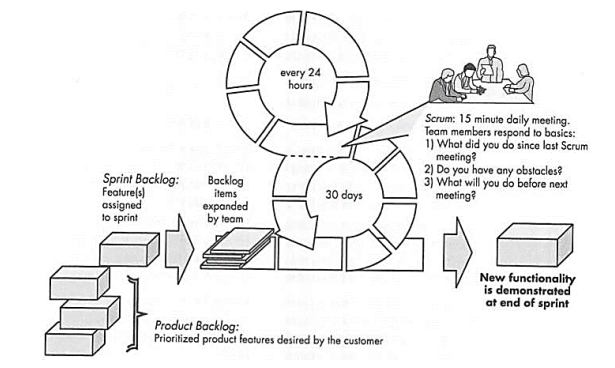
\includegraphics [width = 12.5cm, height= 8cm]{gambar/alur_proses_scrum}}
\caption{Alur Proses Scrum \citep{pressman2010}}
\label{alur_proses_scrum}
\end{figure}	

\par Menurut \cite{pressman2010}, di setiap tahap pengembangan, terjadi aktivitas kerja yang terlingkup di dalam suatu pola proses yang dinamakan sprint. Setiap pola proses yang terjadi, akan terdapat seperangkat kegiatan berikut: 

\begin{enumerate}[a.]
\item \textit{Backlog}
 \par Sebuah rincian prioritas pada fitur-fitur yang akan dibangun pada suatu proyek. Isi pada fitur dapat ditambahkan setiap saat. 
 \item \textit{Sprints} 
 \par Kumpulan aktivitas kerja yang dilakukan untuk memenuhi kebutuhan yang ditetapkan dalam backlog dan harus diselesaikan pada waktu yang telah ditentukan. Perubahan tidak dapat dilakukan pada proses sprintsehingga setiap tim akan bekerja di dalam lingkungan yang stabil. 
 \item \textit{Scrum Meeting} 
 \par Pertemuan yang dilakukan setiap hari oleh tim scrum untuk membahas apa yang telah dikerjakan sejak pertemuan terakhir, merencanakan dan membahas masalah-masalah yang ada (biasanya 15 menit).
 \item \textit{Demos} 
 \par Menujukan hasil fungsionalitas yang telah diimplementasikan sehingga dapat dievaluasi oleh pengguna. 
 Demo harus berupa fitur-fitur yang telah diselesaikan sesuai dengan waktu yang telah ditetapkan. 
\end{enumerate}

\section{\uppercase{Black Box Testing}}
Pengujian \textit{blackbox (blackbox testing)} adalah salah satu metode pengujian perangkat lunak yang berfokus pada sisi fungsionalitas, khususnya pada input dan output aplikasi (apakah sudah sesuai dengan apa yang diharapkan atau belum). Tahap pengujian atau testing merupakan salah satu tahap yang harus ada dalam sebuah siklus pengembangan perangkat lunak (selain tahap perancangan atau desain) \citep{iskandaria2012}. Menurut \cite{shihab2011} kategori kesalahan/error yang akan diketahui melalui black box testing :

\begin{itemize}
\item Fungsi yang hilang atau tak benar/salah
\item Error dari antar-muka/interface
\item Error dari struktur data atau akses eksternal database
\item Error dari kinerja atau tingkah laku/perform
\item Error dari inisialisasi dan terminasi
\end{itemize}


\section{\uppercase{System Usability Scale (SUS)}}
\textit{System Usability Scale} adalah sebuah metode uji pengguna yang digunakan untuk mengukur \textit{usability}. John Brooke mengembangkan \textit{System Usability Scale} pada tahun 1986 sebagai metode yang menyediakan alat ukur bersifat \textit{“quick and dirty”}. Menurut Brooke, \textit{System Usability Scale} memungkinkan untuk mengevaluasi berbagai macam produk dan jasa, termasuk hardware, software, website dan aplikasi. 

\par Metode penilaian System Usability Scale mengharuskan para peserta untuk memberikan tanggapan terhadap 10 item pernyataan menggunakan 5 poin skala Likert. Responden diminta untuk memberikan penilaian dari skala 1 yang berarti “Sangat tidak setuju”, skala 2 yang berarti “Tidak setuju”, skala 3 yang berarti “Netral”, skala 4 yang berarti “Setuju”, dan skala 5 yang berarti “Sangat setuju”. Jika karena alasan tertentu, Jika responden merasa tidak menemukan skala respon yang tepat, responden harus mengisi titik tengah skala pengujian. System Usability Scale dipercaya skala yang dapat digunakan untuk dua faktor yang berbeda, yaitu mengukur keseluruhan dari usability (8 dari 10 item) dan mengukur learnability 
(2 dari 10 item) dari suatu sistem. 

\par Adapun 10 item pertanyaan kuesioner yang digunakan dalam metode ini :

\begin{table}[H]
\centering
\caption{Item Pernyataan System Usability Scale \citep{bangor2008, finstad2006}}
\label{item_pernyataan_system_usability_scale}
\begin{tabular}{|l| >{\centering\arraybackslash} m{10cm}| >{\centering\arraybackslash} m{2cm}|} 
\hline
\textbf{No.} & \textbf{Pernyataan} & \textbf{Skala}  \\ 
\hline
1.           & Saya pikir bahwa saya akan ingin lebih sering menggunakan aplikasi ini      & 1 s/d 5   \\ 
\hline
2.           & Saya merasa sistem ini tidak harus dibuat serumit ini		& 1 s/d 5  \\ 
\hline
3.           & Saya pikir sistem ini mudah digunakan     		& 1 s/d 5   \\ 
\hline
4.           & Saya pikir saya perlu bantuan tenaga teknis agar dapat menggunakan sistem ini      		& 1 s/d 5      \\ 
\hline
5.           & Saya meneukan berbagai fungsi pada sistem ini terintegrasikan dengan baik        	& 1 s/d 5   \\
\hline
6.           & Saya pikir ada terlalu banyak ketidaksesuaian dalam sistem ini   & 1 s/d 5   \\
\hline
7.           & Saya bayangkan bahwa kebanyakan orang akan belajar menggunakan sistem dengan cepat    & 1 s/d 5   \\
\hline
8.           & Saya menemukan bahwa sistem sangat rumit digunakan   & 1 s/d 5   \\
\hline
9.           & Saya merasa sangat percaya diri untuk menggunakan sistem ini   & 1 s/d 5   \\
\hline
10.           & Saya perlu belajar banyak hal sebelum saya bisa 
menggunakan sistem ini   & 1 s/d 5   \\
\hline
\end{tabular}
\end{table}

%-----------------------------------------------------------------------------%

% Baris ini digunakan untuk membantu dalam melakukan sitasi
% Karena diapit dengan comment, maka baris ini akan diabaikan
% oleh compiler LaTeX.

\fancyhf{} 
\fancyfoot[R]{\thepage}

\begin{comment}
\bibliography{daftar-pustaka}
\end{comment}


%-------------------------------------------------------------------------------
%                            BAB III
%               		METODOLOGI PENELITIAN
%-------------------------------------------------------------------------------
\fancyhf{} 
\fancyfoot[C]{\thepage}
\chapter{METODOLOGI PENELITIAN}

\section{\uppercase{WAKTU DAN LOKASI PENELITIAN}}
Penelitian ini dilaksanakan di Ruang D3 Manajemen Agribisnis Fakultas Pertanian Universitas Syiah Kuala. Waktu yang dibutuhkan untuk penelitian ini adalah 8 bulan, yang dimulai dari bulan Juni 2021 hingga Januari 2022.

\section{\uppercase{JADWAL PELAKSANAAN PENELITIAN}}
Jadwal pelaksanaan penelitian secara detail dapat dilihat pada Tabel \ref{tab:jadwal}

\begin{table}[H]
	\begin{center}
	\caption{Jadwal Pelaksanaan Penelitian}
	\label{tab:jadwal}
	% \footnotesize
	\begin{tabular}{|c|l|c|c|c|c|c|c|c|c|}
	\hline
	\multirow{2}{*}{No.}&\multirow{2}{*}{Jenis Kegiatan}&\multicolumn{8}{c|}{Bulan}\\
	\cline{3-10}
	&&Jun&Jul&Agu&Sep&Okt&Nov&Des&Jan\\
	\hline
	1&Studi Literatur&\cellcolor{gray}&\cellcolor{gray}&&&&&&\\
	\hline
	2&Penulisan Proposal&&&\cellcolor{gray}&\cellcolor{gray}&&&&\\
	\hline
	3&Pengembangan Aplikasi&&&\cellcolor{gray}&\cellcolor{gray}&\cellcolor{gray}&&&\\
	\hline
	4&Evaluasi Sistem&&&&&&\cellcolor{gray}&\cellcolor{gray}&\\
	\hline
	5&Penulisan Laporan Akhir&&&&&&&&\cellcolor{gray}\\
	\hline
	\end{tabular}
	% \normalsize
	\end{center}
\end{table}

\section{\uppercase{ALAT DAN BAHAN}}
Alat dan Bahan yang akan digunakan pada penelitian ini terdiri dari beberapa perangkat keras (\textit{hardware}) dan perangkat lunak (\textit{software}) yang dijabarkan sebagai berikut:

\begin{enumerate}
\item Perangkat Keras
	\begin{itemize}
	\item Laptop Dell Inspiron 15 7000 dengan spesifikasi RAM 12GB, Intel(R) Core(TM) i5-7300HQ CPU @2.5GHz, HDD 1TB dan SSD 250 GB.
	\end{itemize}

\item Perangkat Lunak
	\begin{itemize}
	\item Sistem Operasi Windows 10
	\item Figma
	\item Visual Studio Code v1.60.1
	\item XAMPP v3.2.4
	\item Brave Browser v1.29.81
	\item Potsman v8.10
	\end{itemize}
\end{enumerate}

\section{\uppercase{METODE PENELITIAN}}
Metode penelitian yang dilakukan akan terdiri dari beberapa tahapan. Skema dari alur tahapan tersebut dapat dilihat pada Gambar \ref{alur_penelitian}.

\begin{figure}[H]
\centering
{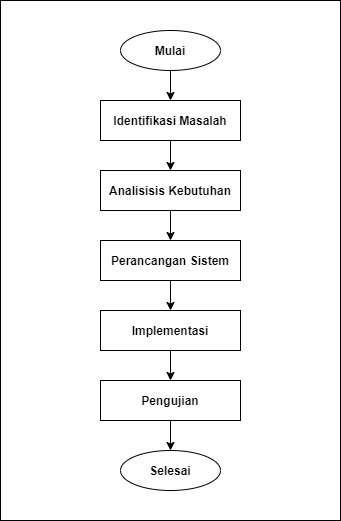
\includegraphics [width = 8cm, height= 11cm]{gambar/flowchart_proposal}}
\caption{Diagram Alir Penelitian}
\label{alur_penelitian}
\end{figure}

\par Adapun untuk metode pengembangan aplikasinya menggunakan metode pengembangan Scrum. Metode Scrum diimplementasikan pada tahapan analisis kebutuhan, perancangan sistem, implementasi, serta pengujian.

\fancyhf{} 
\fancyfoot[R]{\thepage}

\subsection{Identifikasi Masalah}
Tahapan ini merupakan tahapan yang dilakukan untuk mengidentifikasi masalah yang dihadapi pada sistem pemasaran saat ini, sehingga dari permasalahan yang didapatkan menjadi landasan untuk penelitian ini. Masalah-masalah yang berhasil diidentifikasi adalah sebagai berikut:

\begin{itemize}
	\item Sistem pemasaran saat ini masih dilakukan secara datang langsung ke tempat penjualan atau memesan lewat aplikasi media sosial.
	\item Pelanggan tidak dapat mengetahui ketersediaan stok produk sebelum bertanya kepada penjual atau mengunjungi langsung tempat penjualannya.
	\item Susahnya menjaga kestabilan harga produk antar penjual tanaman hidroponik.
\end{itemize}

\subsection{Analisis Kebutuhan}
Tahapan analisis kebutuhan dilakukan untuk mengetahui kebutuhan pengguna dan kebutuhan sistem serta fungsi apa saja yang akan dibangun nantinya didalam aplikasi. Kebutuhan tersebut dibagi menjadi dua yaitu kebutuhan fungsional yang mendefinisikan fungsionalitas dari sebuah sistem dan kebutuhan non-fungsional yang menjadi batasan kebutuhan yang tidak dapat dikerjakan oleh sistem itu sendiri. Setiap kebutuhan-kebutuhan tersebut akan dijabarkan sebagai berikut:

\begin{enumerate}[a.]
	\item Kebutuhan Fungsional
		\begin{itemize}
		\item Aplikasi berbasis web mampu mendaftarkan akun admin dan penjual.
		\item Aplikasi berbasis web mampu menampilkan jumlah dan informasi pengguna, produk, pesanan, ulasan dan laporan dari pembeli.
		\item Aplikasi berbasis web mampu mengelola promo dan produk seperti menambah, mengubah atau menghapus promo dan produk.
		\item Aplikasi berbasis web mampu memblokir penjual yang melakukan pelanggaran.
		\item Aplikasi berbasis web mampu meninjau pesanan yang masuk dari pembeli.
		\end{itemize}
	
	\item Kebutuhan Non-Fungsional
		\begin{itemize}
		\item Aplikasi berbasis web dapat diakses oleh superadmin, admin dan penjual dengan syarat adanya koneksi internet.
		\item Aplikasi berbasis web untuk saat ini hanya terbatas untuk wilayah kota Banda Aceh.
		\item Aplikasi berbasis web tidak dapat menerima pembayaran, karena pembayaran dilakukan secara tunai atau \textit{cash on delivery} (COD).
		\end{itemize}
	\end{enumerate}

\par Melalui kebutuhan-kebutuhan di atas maka dibangunlah \textit{use case diagram} yang dapat dilihat pada gambar \ref{use_case_diagram}.

\begin{figure}[H]
	\centering
	{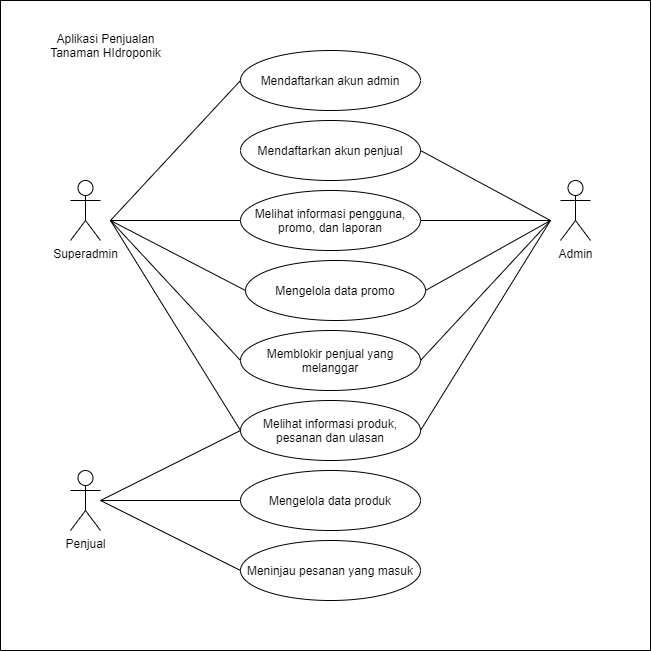
\includegraphics [width = 14cm, height= 14cm]{gambar/use_case_diagram}}
	\caption{Use Case Diagram}
	\label{use_case_diagram}
\end{figure}

\subsection{Perancangan Sistem}
Tahap perancangan sistem dibuat berdasarkan hasil yang telah didapatkan dari analisis kebutuhan. Kemudian dirancang sistem agar dapat berjalan dengan baik, dimulai dari perancangan prototipe menggunakan Figma, selanjutnya perancangan \textit{database} menggunakan \textit{Entity Relationship Diagram} (ERD), dan perancangan \textit{Business Diagram} sampai rancangan alur kerja sistem. \textit{Business Diagram} dapat dilihat pada Gambar \ref{bisnis_diagram}.

\begin{figure}[H]
\centering
{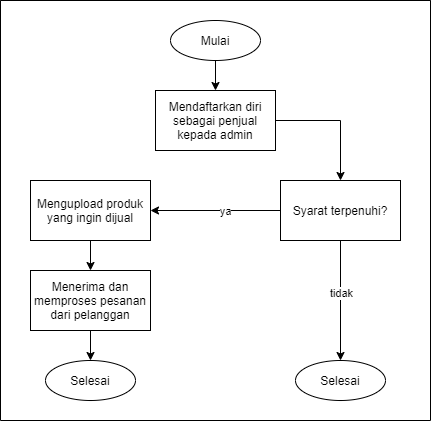
\includegraphics [width = 14cm, height= 10cm]{gambar/bisnis_diagram}}
\caption{Business Diagram}
\label{bisnis_diagram}
\end{figure}

Adapun alur kerja sistem dapat dilihat pada Gambar \ref{alur_kerja_sistem}.

\begin{figure}[H]
\centering
{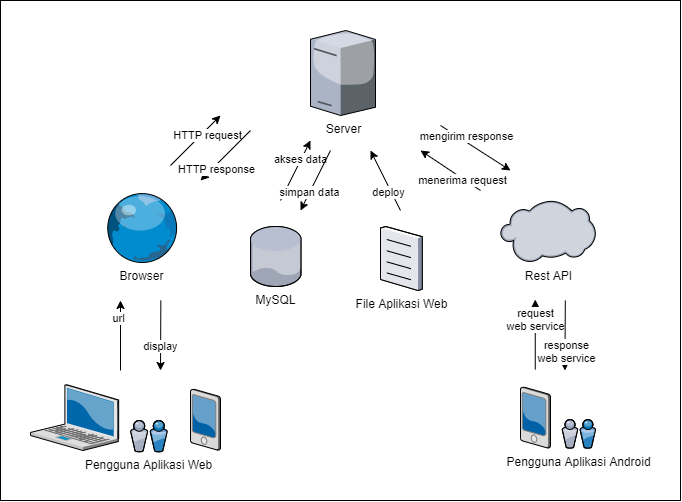
\includegraphics [width = 14cm, height= 10cm]{gambar/alur_kerja_sistem}}
\caption{Alur Kerja Sistem}
\label{alur_kerja_sistem}
\end{figure}

\subsection{Implementasi}
Setelah rancangan sistem selesai dilakukan, selanjutnya akan diimplementasikan hasil rancangan tersebut ke dalam bentuk kode pemrograman. Pada tahap ini aplikasi berbasis web akan dibangun menggunakan \textit{framework} Laravel dan MySQL sebagai \textit{database}. Selain Laravel juga digunakan \textit{library} tambahan di dalamnya yaitu Livewire. Livewire merupakan \textit{full-stack framework} untuk Laravel yang berguna untuk membuat tampilan antarmuka menjadi dinamis. Alasan penggunaan Livewire didalam penelitian ini supaya tidak perlu membuat terpisah antara \textit{front end} dan \textit{back end} sehingga akan mempercepat proses pengembangan aplikasi. Kemudian dari aplikasi web ini nantinya akan dibuatkan REST API untuk aplikasi Android agar dapat mengakses dan mengirimkan data ke dalam server.

\subsection{Pengujian}
Pengujian sistem sangat diperlukan untuk memastikan sistem yang sudah dibangun dapat berjalan sesuai dengan apa yang diharapkan. Pada penelitian ini akan dilakukan 2 pengujian yaitu pengujian fungsionalitas dan pengujian \textit{usability}.

\begin{enumerate}
	\item Pengujian Fungsionalitas
	\par Pengujian Fungsionalitas dilakukan dengan menggunakan metode \textit{Black Box}. Metode ini berfokus pada fungsionalitas dari aplikasi yang telah dibuat dengan cara menguji aplikasi tersebut apakah sudah berjalan sesuai yang diharapkan atau belum, seperti menguji fungsi-fungsi pada aplikasinya, \textit{input output} yang dihasilkan, serta dalam mengakses data.
	\item Pengujian \textit{Usability}
	\par Pengujian \textit{Usability} dilakukan dengan menggunakan metode \textit{Usability Metric for User Experience} (UMUX). Pengujian ini dilakukan untuk menguji aplikasi yang sudah dibuat apakah sudah sesuai dengan kebutuhan pengguna serta mudah untuk digunakan dan dipahami oleh pengguna aplikasi. Pengujian akan dilakukan dengan membagikan kuesioner kepada beberapa sampel pengguna yang akan menggunakan aplikasi. Nantinya dari hasil kuesioner tersebut akan didapatkan hasil apakah aplikasi dikatakan layak digunakan atau tidak. 
\end{enumerate}

%-----------------------------------------------------------------------------%

% Baris ini digunakan untuk membantu dalam melakukan sitasi
% Karena diapit dengan comment, maka baris ini akan diabaikan
% oleh compiler LaTeX.
\begin{comment}
\bibliography{daftar-pustaka}
\end{comment}

%-------------------------------------------------------------------------------
%                            BAB IV
%               		HASIL DAN PEMBAHASAN
%-------------------------------------------------------------------------------
\fancyhf{} 
\fancyfoot[C]{\thepage}
\chapter{HASIL DAN PEMBAHASAN}

\section{\uppercase{Analisis Kebutuhan}}
Analisis kebutuhan merupakan tahapan yang dilakukan untuk mengetahui pengguna yang terlibat dalam aplikasi yang akan dibangun serta mengetahui kebutuhan-kebutuhan dari setiap pengguna supaya memperjelas tujuan dari pembuatan aplikasi kedepannya. Hasil daripada analisis kebutuhan dapat dilihat dibawah ini:

\subsection{Kategori Pengguna}
Pengguna yang akan menggunakan aplikasi web ini dapat dikelompokkan menjadi dua ketegori, yaitu:

\begin{enumerate}
	\item Admin
		\par Admin adalah orang yang mengelola aplikasi seperti mendaftarkan akun penjual baru, membuat promo diaplikasi dan memantau pengguna.
	
	\item Penjual
		 \par Penjual adalah kelompok pengguna yang menggunakan aplikasi bertujuan untuk menjual produknya yaitu tanaman hidroponik kepada calon pembeli.
\end{enumerate}

\subsection{Kebutuhan Pengguna}
Setelah mengetahui kategori pengguna, selanjutnya dilakukan analisis kebutuhan untuk setiap pengguna dengan cara dibuatkan tabel \textit{user story} berdasarkan masing-masing pengguna. Berikut tabel \textit{user story}nya.

\begin{table}[H]
	\begin{center}
	\caption{\textit{User Story}}
	\label{tab:user story}
	% \footnotesize
	\begin{tabular}{|c| m{12cm} |}
	\hline
	{\footnotesize Sebagai} & \multicolumn{1}{c|}{{\footnotesize \textit{User Story}}}\\
	\hline
	\multirow{8}{*}{\footnotesize Admin} & {\footnotesize Saya sebagai admin bisa mendaftarkan akun penjual}\\
	\cline{2-2}& {\footnotesize Saya sebagai admin ingin menambahkan promo di aplikasi}\\
	\cline{2-2}& {\footnotesize Saya sebagai admin ingin melihat semua produk yang dijual di aplikasi}\\
	\cline{2-2}& {\footnotesize Saya sebagai admin ingin melihat semua pesanan yang terjadi di aplikasi}\\
	\cline{2-2}& {\footnotesize Saya sebagai admin ingin melihat semua pengguna yang terdaftar}\\
	\cline{2-2}& {\footnotesize Saya sebagai admin ingin melihat semua keluhan dari pembeli}\\
	\cline{2-2}& {\footnotesize Saya sebagai admin ingin melihat semua ulasan yang diberikan pembeli}\\
	\cline{2-2}& {\footnotesize Saya sebagai admin bisa memblokir akun penjual yang melakukan pelanggaran}\\
	\hline
	\end{tabular}
	% \normalsize
	\end{center}
\end{table}

\newpage

\addtocounter{table}{-1}
\begin{table}[H]
	\begin{center}
	% \caption{User Story}
	% \label{tab:user story}
	% \footnotesize
	\begin{tabular}{|c| m{12cm} |}
	\hline
	\multirow{5}{*}{\footnotesize Penjual} & {\footnotesize Saya sebagai penjual ingin menambahkan produk yang ingin dijual}\\
	\cline{2-2}& {\footnotesize Saya sebagai penjual ingin mengubah atau menghapus produk yang saya jual}\\
	\cline{2-2}& {\footnotesize Saya sebagai penjual ingin menerima pesanan dari pembeli}\\
	\cline{2-2}& {\footnotesize Saya sebagai penjual ingin melihat detail pesanan dan mengubah statusnya}\\
	\cline{2-2}& {\footnotesize Saya sebagai penjual ingin melihat ulasan dari pembeli terhadap produk saya}\\
	\hline
	{\footnotesize Pengguna} & {\footnotesize Saya sebagai pengguna ingin mengubah profil akun saya}\\
	\hline
	\end{tabular}
	% \normalsize
	\end{center}
\end{table}

\section{\uppercase{Perancangan Sistem}}

\subsection{\textit{Use Case Diagram}}
\textit{Use case diagram} adalah diagram yang menjelaskan interaksi antara pengguna atau yang disebut aktor dengan sistem. Selain itu \textit{Use case diagram} juga memperlihatkan fitur apa saja yang dapat dilakukan oleh sistem. Berikut merupakan gambaran \textit{Use case diagram} untuk aplikasi penjualan tanaman hidroponik berbasis web :

\begin{figure}[H]
	\centering
	{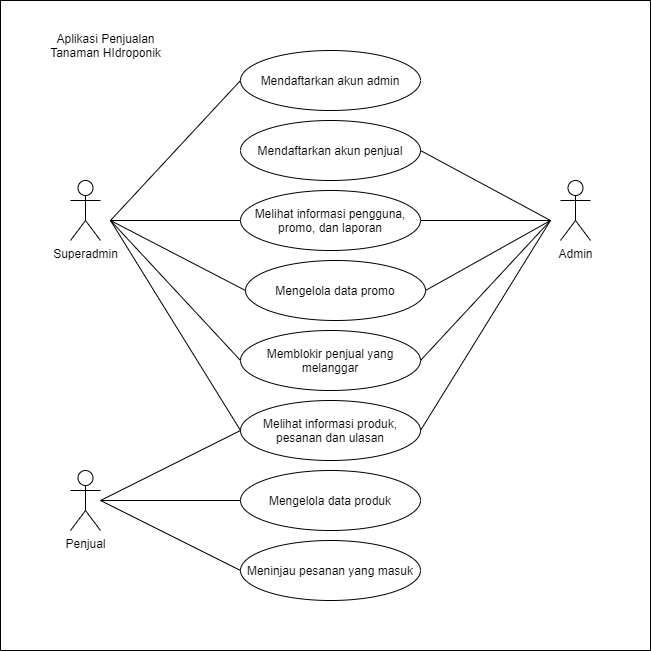
\includegraphics [width = 13cm, height= 13cm]{gambar/use_case_diagram}}
	\caption{\textit{Use Case Diagram}}
	\label{use_case_diagram}
\end{figure}

\par Gambar \ref*{use_case_diagram} merupakan\textit{ Use case diagram} yang menjelaskan interaksi antara superadmin, admin dan penjual dengan sistem aplikasi. Dimana level yang paling tinggi di sistem ini adalah superadmin yang bertindak untuk mendaftarkan admin, lalu nantinya para admin inilah yang bertugas mendaftarkan para penjual yang ingin menjual produknya di aplikasi AgriHub ini. Superadmin dan admin disini dapat memantau informasi semua pengguna yang sudah terdaftar diaplikasi baik itu penjual maupun pembeli yang mendaftar lewat aplikasi android dan dapat melihat produk-produk apa saja yang telah diunggah oleh para penjual, serta dapat menghapusnya jika dianggap tidak sesuai. Superadmin dan admin juga dapat melihat semua pesanan yang sudah terjadi antara penjual dengan pembeli, melihat ulasan dari pembeli terhadap produk yang dibeli dari penjual serta dapat mengadakan promo sesekali di aplikasinya dan dapat melihat laporan yang masuk dari pembeli terhadap penjual serta dapat mengambil tindakan seperti memblokir penjual tersebut dari sistem.

\par Sedangkan dari sisi aktor penjual. Setelah penjual didaftarkan oleh admin, penjual harus memverifikasi emailnya terlebih dahulu sebelum bisa menggunakan aplikasinya. Baru setelah verifikasi email penjual dapat menggunakan aplikasinya untuk menambahkan produk yang ingin dijualnya, mengelolanya seperti mengubah dan menghapus produk, menerima pesanan dari pembeli dan mengubah statusnya dari belum menjadi diproses, dikirim dan sampai selesai. Penjual juga dapat melihat ulasan-ulasan dari pembeli terhadap pesanan dan produk yang ia jual di aplikasi.

\subsection{\textit{Business Diagram}}
\textit{Business diagram} merupakan diagram yang menggambarkan alur proses bisnis yang berjalan dari sebuah sistem. \textit{Business diagram} dapat membuat alur proses bisnis menjadi lebih sederhana sehingga mudah dipahami oleh semua orang. \textit{Business diagram} juga dapat dibuat secara umum dengan hanya berfokus pada proses bisnis inti saja. Pada rancangan \textit{business diagram} ini, proses bisnis inti terdiri dari :

\begin{enumerate}
	\item Mendaftarkan diri sebagai penjual kepada admin
	\item Memverifikasi email yang sudah didaftarkan admin
	\item Menambahkan produk yang ingin dijual
	\item Menerima dan memproses pesanan.
\end{enumerate}

Untuk \textit{Business Diagram} dapat dilihat pada Gambar \ref{bisnis_diagram}.

\begin{figure}[H]
	\centering
	{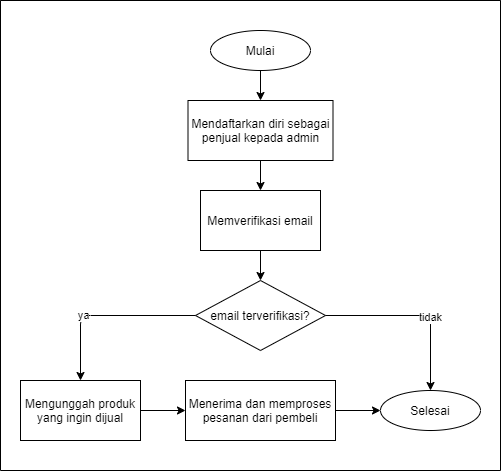
\includegraphics [width = 12cm, height= 10cm]{gambar/bisnis diagram baru}}
	\caption{\textit{Business Diagram}}
	\label{bisnis_diagram}
\end{figure}

Gambar 4.2 memperlihatkan alur bisnis di dalam sistem. Dimulai ketika pengguna ingin mendaftarkan diri sebagai penjual kepada admin, kemudian admin meminta datanya beserta email yang valid dari penjual untuk didaftarkan di sistem. Setelah datanya didaftarkan maka penjual harus memverifikasi emailnya terlebih dahulu sebelum bisa menggunakan aplikasi, setelah terverifikasi maka proses bisnis selanjutnya adalah penjual menjual produknya di dalam sistem. Tahapan tersebut penting agar produk dari penjual dapat dilihat dan dipesan oleh pembeli. Setelah pembeli membeli atau memesan produk, tahapan selanjutnya adalah penjual menerima dan memproses pesanan dari pembeli.
	
\subsection{\textit{Activity Diagram}}
\textit{Activity Diagram} merupakan salah satu diagram yang menggambarkan langkah-langkah alur yang lebih rinci dari sistem. \textit{Activity Diagram} mempunyai titik mulai dan titik selesai yang di dalamnya menjelaskan berbagai alur kerja sistem secara beruntun. Biasanya \textit{Activity
Diagram} digunakan oleh pengembang aplikasi untuk memahami alur program yang akan dibuat. Berikut merupakan activity diagram dalam penelitian ini :

\newpage

\begin{enumerate}
	\item \textit{Activity Diagram} Masuk Akun
	\begin{figure}[H]
		\centering
		{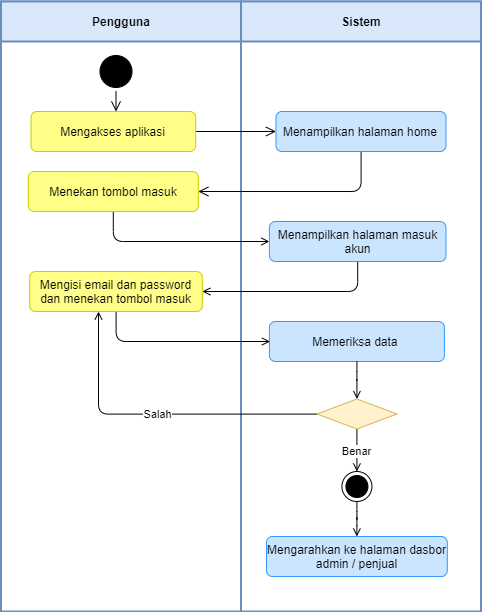
\includegraphics [width = 8cm, height= 10.5cm]{gambar/activity diagram/masuk akun}}
		\caption{\textit{Activity Diagram} Masuk Akun}
		\label{masuk akun}
	\end{figure}
	\par Gambar \ref*{masuk akun} memperlihatkan aktivitas ketika pengguna ingin masuk akun atau \textit{login} ke dalam sistem. Pengguna mengakses aplikasi terlebih dahulu dan menekan tombol masuk lalu mengisi data seperti \textit{email} dan \textit{password} yang kemudian akan diperiksa oleh sistem.

	\item \textit{Activity Diagram} Melihat Produk
	\begin{figure}[H]
		\centering
		{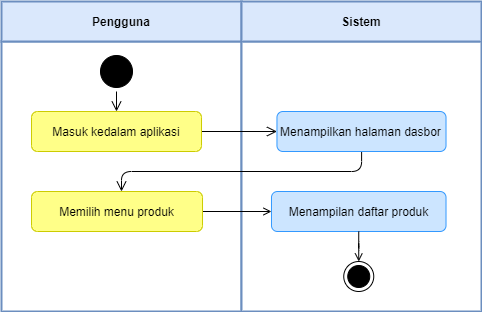
\includegraphics [width = 8cm, height= 6cm]{gambar/activity diagram/lihat produk}}
		\caption{\textit{Activity Diagram} Melihat Produk}
		\label{lihat produk}
	\end{figure}
	\par Gambar \ref*{lihat produk} memperlihatkan aktivitas ketika pengguna baik itu admin maupun penjual ketika hendak melihat daftar produk. Pengguna harus terlebih dahulu masuk kedalam aplikasi lalu memilih menu produk, maka akan tampil halaman daftar semua produk yang dijual disistem bagi sisi admin dan akan tampil halaman daftar produk yang ia jual bagi sisi penjual.

	\item \textit{Activity Diagram} Menambahkan Produk
	\begin{figure}[H]
		\centering
		{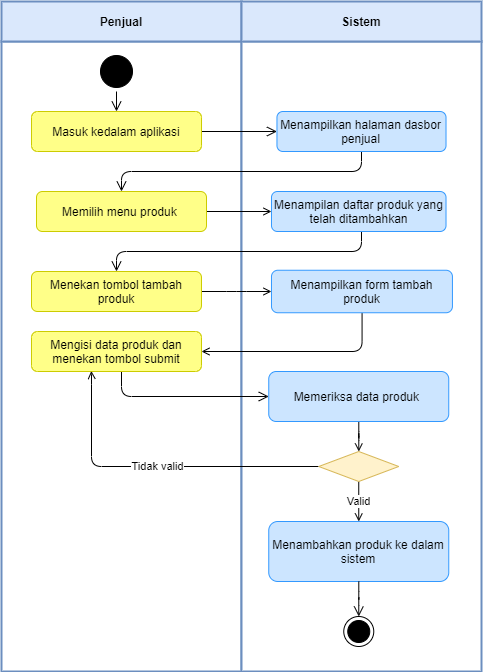
\includegraphics [width = 8cm, height= 11cm]{gambar/activity diagram/jual produk}}
		\caption{\textit{Activity Diagram} Menambahkan Produk}
		\label{jual produk}
	\end{figure}
	\par Gambar \ref*{jual produk} memperlihatkan aktivitas ketika penjual hendak menambahkan produk ke dalam sistem. Aktivitas ini hanya bisa dilakukan oleh penjual dan sudah melakukan aktivitas masuk akun (\textit{login}). Pada halaman produk penjual dapat menambahkan produk dengan menekan tombol tambah, lalu sistem akan menampilkan \textit{form} data produk untuk diisi oleh penjual. Setelah penjual mengisi semua data mengenai produk baru lalu menekan tombol \textit{submit}, maka sistem akan menvalidasi datanya. Apabila bila data yang diinput valid maka proses tambah produk berhasil dan data tersebut akan disimpan di sistem.

	\newpage
	\item \textit{Activity Diagram} Mengubah atau Menghapus Produk
	\begin{figure}[H]
		\centering
		{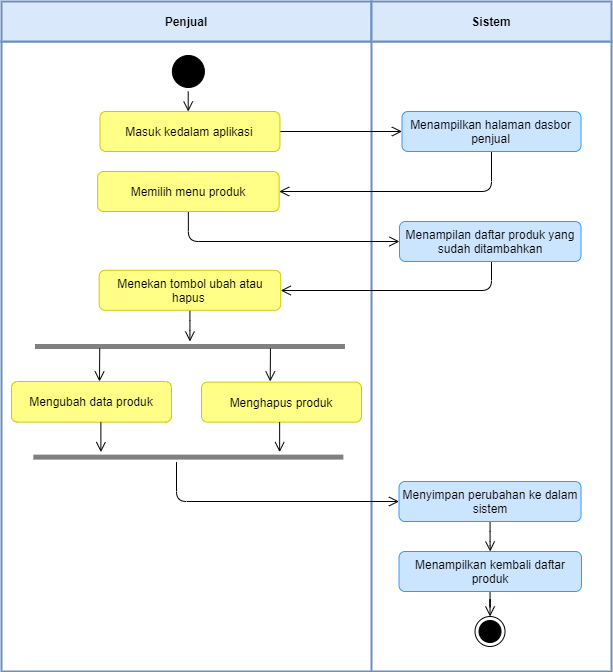
\includegraphics [width = 8cm, height= 11cm]{gambar/activity diagram/ubah atau hapus produk}}
		\caption{\textit{Activity Diagram} Mengubah atau Menghapus Produk}
		\label{ubah atau hapus produk}
	\end{figure}
	\par Gambar \ref*{ubah atau hapus produk} memperlihatkan aktivitas ketika penjual hendak mengubah atau menghapus produk yang dia jual di sistem. Penjual dapat mengubah data produk seperti gambar, nama, harga, stok dan data lainnya atau penjual bisa juga menghapus produknya dari sistem jika diinginkan.

	\item \textit{Activity Diagram} Melihat Pesanan
	\begin{figure}[H]
		\centering
		{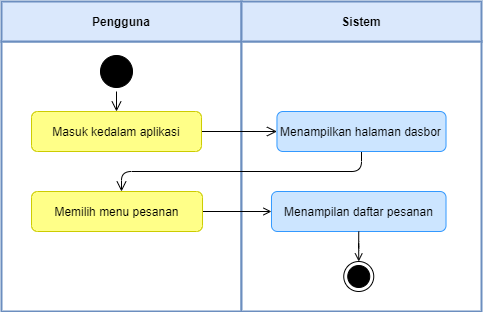
\includegraphics [width = 8cm, height= 6cm]{gambar/activity diagram/lihat pesanan}}
		\caption{\textit{Activity Diagram} Melihat Pesanan}
		\label{lihat pesanan}
	\end{figure}
	\par Gambar \ref*{lihat pesanan} memperlihatkan aktivitas ketika pengguna baik itu admin maupun penjual ketika hendak melihat daftar pesanan. Pengguna harus terlebih dahulu masuk kedalam aplikasi lalu memilih menu pesanan, maka akan tampil halaman daftar semua pesanan yang sudah terjadi disistem bagi sisi admin dan akan tampil halaman daftar pesanan yang dia terima dari pembeli bagi sisi penjual.

	\item \textit{Activity Diagram} Mengubah Status Pesanan
	\begin{figure}[H]
		\centering
		{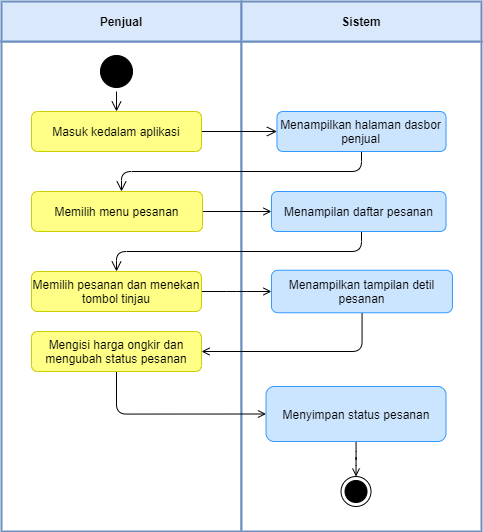
\includegraphics [width = 8cm, height= 11cm]{gambar/activity diagram/ubah status pesanan}}
		\caption{\textit{Activity Diagram} Mengubah Status Pesanan}
		\label{ubah status pesanan}
	\end{figure}
	\par Gambar \ref*{ubah status pesanan} memperlihatkan aktivitas ketika penjual ingin mengubah status pesanan dari pembeli. Penjual memilih terlebih dahulu pesanan yang ingin diproses lalu menekan tombol tinjau dan mengisi harga ongkir pesanan tersebut serta mengubah status pesanannya dari belum menjadi diproses, dikirim, sampai selesai. Penjual juga bisa membatalkan pesanannya dengan mengubah status pesanan menjadi batal.

	\newpage
	\item \textit{Activity Diagram} Membuat Promo
	\begin{figure}[H]
		\centering
		{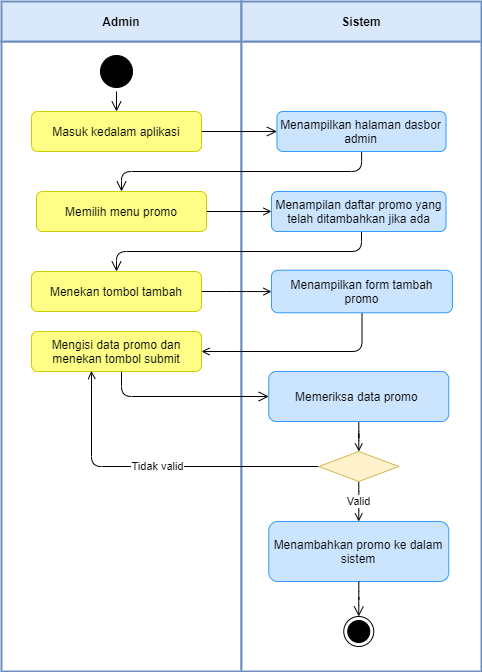
\includegraphics [width = 8cm, height= 12cm]{gambar/activity diagram/buat promo}}
		\caption{\textit{Activity Diagram} Membuat Promo}
		\label{buat promo}
	\end{figure}
	\par Gambar \ref*{buat promo} memperlihatkan aktivitas ketika admin ingin membuat promo di aplikasi. Admin masuk ke aplikasi terlebih dahulu, lalu memilih menu promo dan menekan tombol tambah. Kemudian mengisi data promo seperti gambar, nama promo, potongan, awal periode dan akhir periode. Setelah itu menekan tombol submit maka sistem akan memeriksa datanya. Apabila data yang diinput valid maka proses pembuatan promo berhasil dan promo tersebut dapat digunakan oleh penjual nantinya.

	\newpage
	\item \textit{Activity Diagram} Mengubah atau Menghapus Promo
	\begin{figure}[H]
		\centering
		{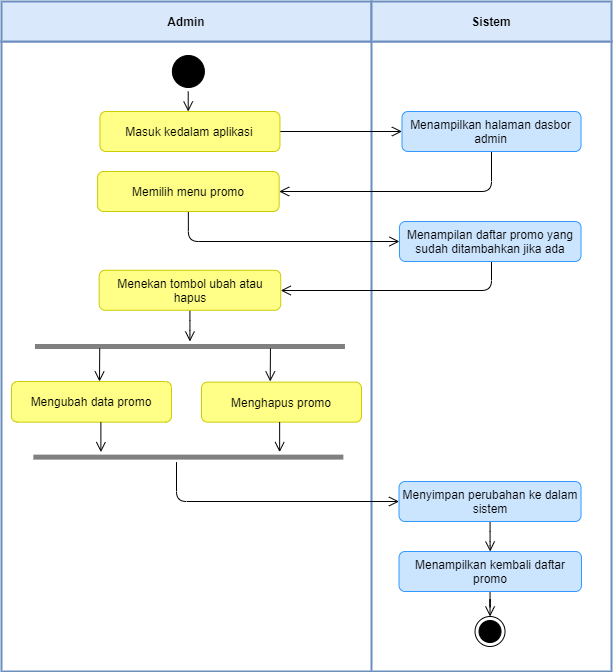
\includegraphics [width = 8cm, height= 11cm]{gambar/activity diagram/ubah atau hapus promo}}
		\caption{\textit{Activity Diagram} Mengubah atau Menghapus Promo}
		\label{ubah atau hapus promo}
	\end{figure}
	\par Gambar \ref*{ubah atau hapus promo} memperlihatkan aktivitas ketika admin hendak mengubah atau menghapus promo yang sedang berlangsung. Admin dapat mengubah data mengenai promo atau menghapusnya. Promo yang sudah melewati tanggal akhir periode akan terhapus otomatis di sistem.

	\item \textit{Activity Diagram} Melihat Pengguna
	\begin{figure}[H]
		\centering
		{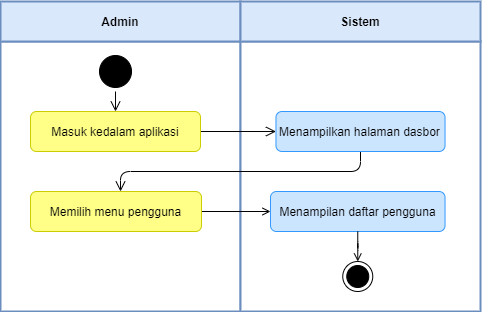
\includegraphics [width = 8cm, height= 6cm]{gambar/activity diagram/lihat pengguna}}
		\caption{\textit{Activity Diagram} Melihat Pengguna}
		\label{lihat pengguna}
	\end{figure}
	\par Gambar \ref*{lihat pengguna} memperlihatkan aktivitas ketika admin ingin melihat semua daftar pengguna yang sudah terdaftar disistem. Admin dapat melakukannya dengan masuk ke aplikasi dan memilih menu pengguna maka akan tampil daftar semua pengguna yang sudah terdaftar disistem baik itu admin, penjual maupun pembeli yang mendaftar lewat aplikasi android.

	\item \textit{Activity Diagram} Mendaftarkan Akun Penjual
	\begin{figure}[H]
		\centering
		{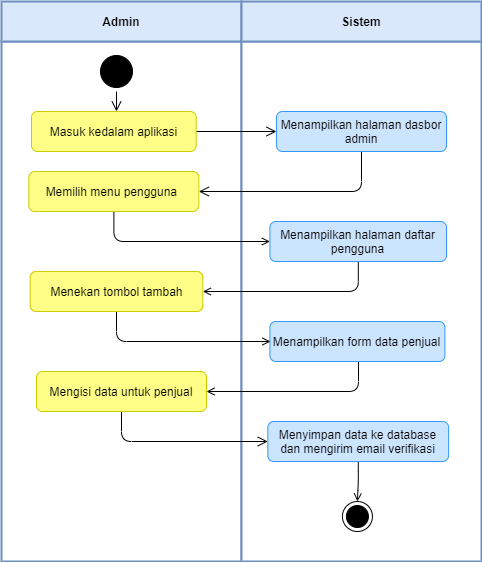
\includegraphics [width = 8cm, height= 11cm]{gambar/activity diagram/daftar akun penjual}}
		\caption{\textit{Activity Diagram} Masuk Akun Penjual}
		\label{daftar akun penjual}
	\end{figure}
	\par Gambar \ref*{daftar akun penjual} memperlihatkan aktivitas ketika admin ingin mendaftarkan akun penjual.
	Admin masuk ke aplikasi lalu memilih menu pengguna dan menekan tombol tambah. Kemudian mengisi data penjual seperti nama, \textit{username, email, password}, nomor hp, alamat dan menekan tombol \textit{submit}. Maka sistem akan menyimpan data penjual di \textit{database} dan mengirimkan \textit{email} verifikasi kepada penjual. Penjual harus menverifikasi \textit{email} tersebut agar dapat menggunakan akun yang sudah didaftarkan admin di aplikasi.

	\newpage
	\item \textit{Activity Diagram} Memblokir Akun Penjual
	\begin{figure}[H]
		\centering
		{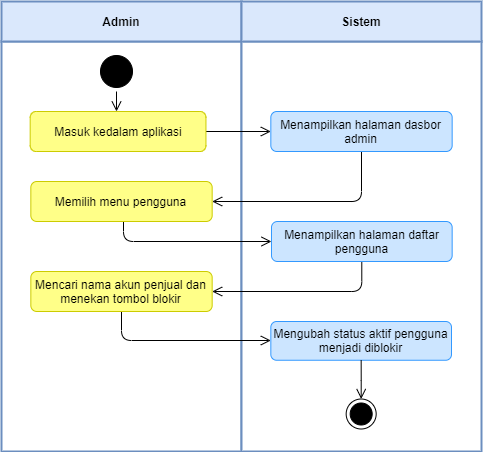
\includegraphics [width = 8cm, height= 10cm]{gambar/activity diagram/blokir penjual}}
		\caption{\textit{Activity Diagram} Memblokir Akun Penjual}
		\label{blokir penjual}
	\end{figure}
	\par Gambar \ref*{blokir penjual} memperlihatkan aktivitas ketika admin hendak memblokir salah satu akun penjual. Admin harus terlebih dahulu masuk kedalam aplikasi, lalu memilih menu pengguna, kemudian mencari pengguna yang ingin diblokir dan menekan tombol blokir. Maka sistem akan mengubah status akun penjual tersebut menjadi diblokir dan penjual tersebut tidak bisa lagi masuk kedalam aplikasi sampai admin mengubah status akunnya kembali.

	\item \textit{Activity Diagram} Melihat Keluhan
	\begin{figure}[H]
		\centering
		{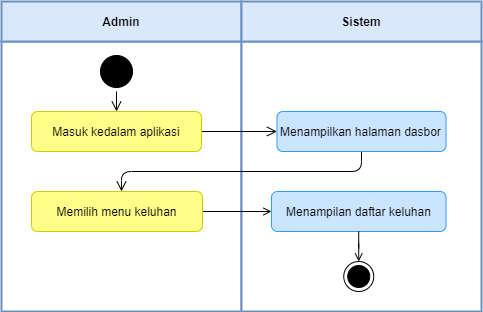
\includegraphics [width = 8cm, height= 6cm]{gambar/activity diagram/lihat keluhan}}
		\caption{\textit{Activity Diagram} Melihat Keluhan}
		\label{lihat keluhan}
	\end{figure}
	\par Gambar \ref*{lihat keluhan} memperlihatkan aktivitas ketika admin ingin melihat semua keluhan yang masuk dari para pembeli terhadap penjual yang terdaftar disistem. Admin dapat melakukannya dengan masuk ke aplikasi dan memilih menu keluhan maka akan tampil daftar semua keluhan yang dikirim oleh pembeli terhadap penjual.

	\item \textit{Activity Diagram} Melihat Ulasan Produk
	\begin{figure}[H]
		\centering
		{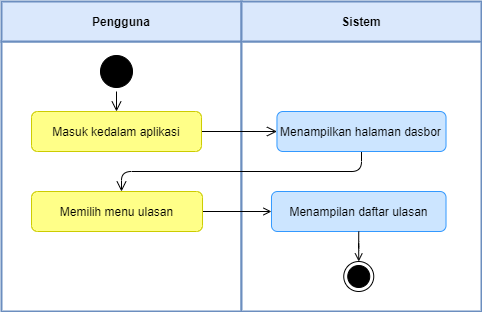
\includegraphics [width = 8cm, height= 5.5cm]{gambar/activity diagram/lihat ulasan}}
		\caption{\textit{Activity Diagram} Melihat Ulasan Produk}
		\label{lihat ulasan}
	\end{figure}
	\par Gambar \ref*{lihat ulasan} memperlihatkan aktivitas ketika pengguna ingin melihat daftar ulasan. Pengguna masuk kedalam aplikasi lalu menekan tombol ulasan, maka akan tampil halaman daftar semua ulasan yang ada disistem bagi sisi admin dan akan tampil halaman daftar ulasan yang dia terima dari pembelinya bagi sisi penjual.

	\item \textit{Activity Diagram} Mengubah Profil Akun
	\begin{figure}[H]
		\centering
		{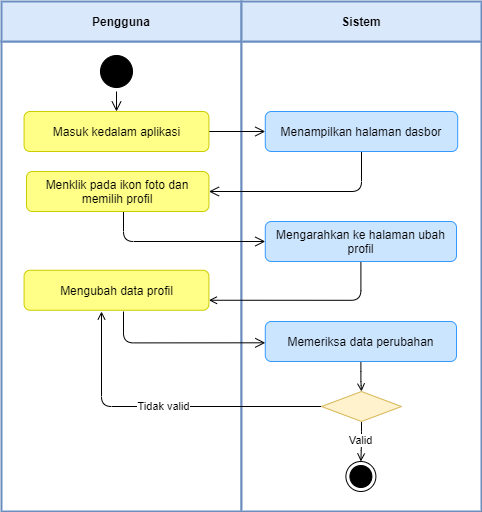
\includegraphics [width = 8cm, height= 7.5cm]{gambar/activity diagram/ubah profil}}
		\caption{\textit{Activity Diagram} Mengubah Profil Akun}
		\label{ubah profil}
	\end{figure}
	\par Gambar \ref*{ubah profil} memperlihatkan aktivitas ketika pengguna ingin mengubah profil akunnya. Pengguna masuk kedalam aplikasi lalu menklik ikon foto dan memilih profil, maka akan diarahkan ke halaman ubah profil. Pengguna dapat mengubah data akunnya seperti foto profil, nama, email, nomor hp, alamat dan password. Setelah selesai melakukan perubahan dan menekan tombol simpan, maka sistem akan memeriksa data perubahannya. Jika data \textit{input}nya valid maka akan disimpan di sistem.
\end{enumerate}

\subsection{\textit{Entity Relationship Diagram}}
\textit{Entity Relationship Diagram} (ERD) merupakan diagram yang menggambarkan hubungan antar data-data yang ada disistem yang saling berelasi satu sama yang lain. \textit{Entity Relationship Diagram} (ERD) dapat dilihat pada Gambar \ref{erd}.

\begin{figure}[H]
	\centering
	{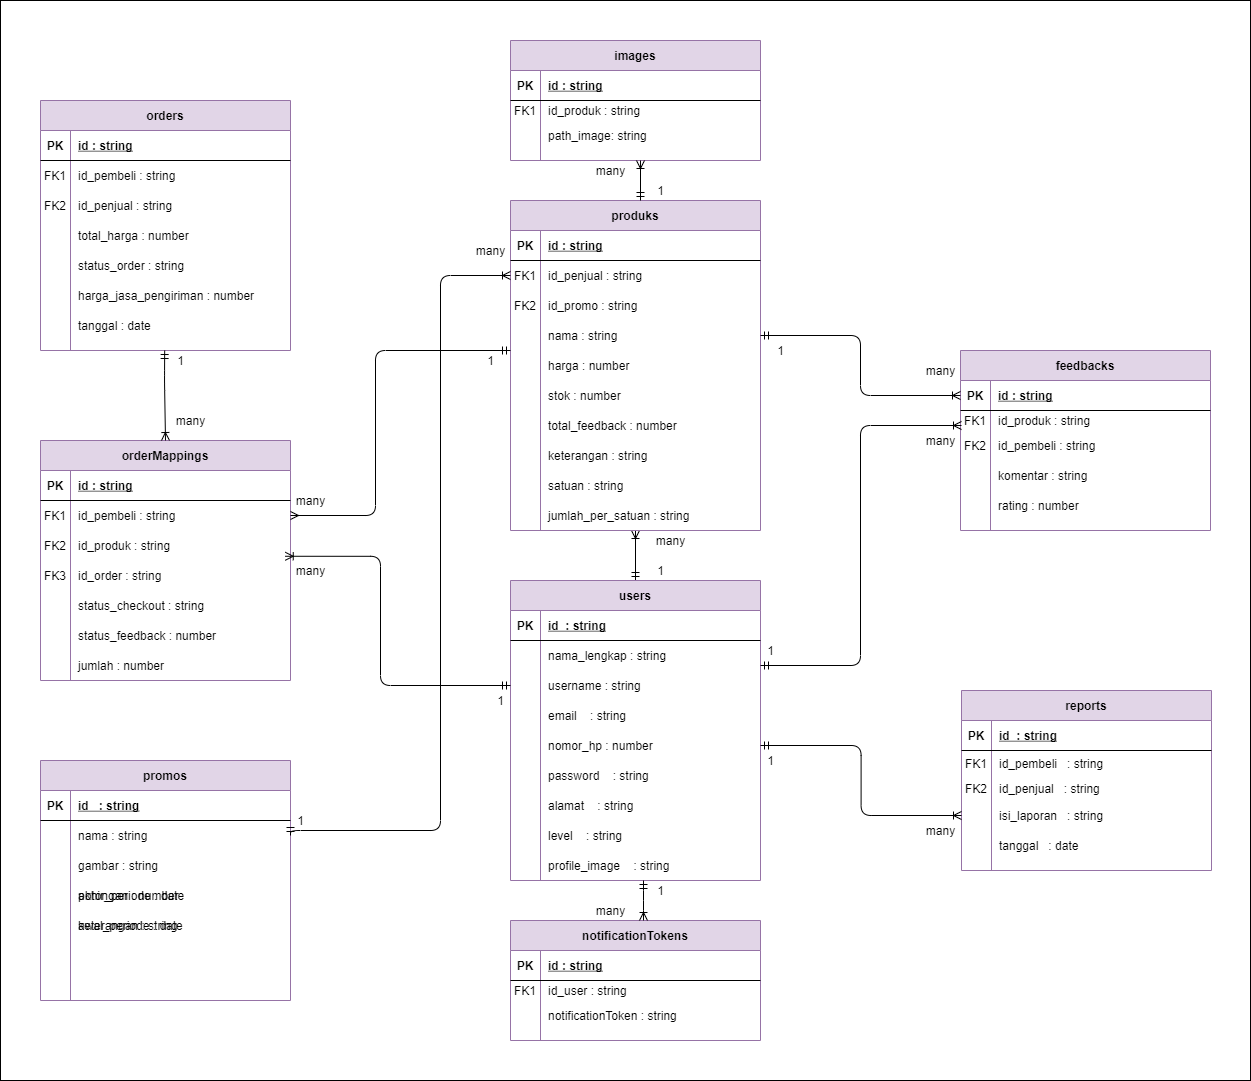
\includegraphics [width = 14.3cm, height= 10.5cm]{gambar/erd}}
	\caption{\textit{Entity Relationship Diagram}}
	\label{erd}
\end{figure}

ERD yang dibuat pada penelitian ini mempunyai 9 entitas. Tiap entitas mempunyai atributnya masing-masing. Relasi antar entitas di dalam sistem ini memiliki kardinalitas (derajat) \textit{one to many}.  Adapun 9 entitas tersebut yang terdiri dari :

\begin{enumerate}
	\newpage
	\item Entitas \textit{users}
	\par Entitas ini akan menyimpan data semua pengguna di dalam aplikasi. Pada entitas \textit{users} terdapat 9 atribut yaitu : id, nama\_lengkap, username, email,
	nomor\_hp, password, alamat, level, dan profile\_image . Atribut id akan menjadi \textit{primary key} serta di dalam entitas ini tidak memiliki \textit{foreign key}.
	\item Entitas \textit{notificationTokens}
	\par Entitas ini akan menyimpan data token ketika pengguna masuk ke dalam aplikasi berbasis android. Pada entitas \textit{notificationTokens} terdapat 3 atribut yaitu : id, notificationToken, dan id\_user . Atribut id akan menjadi \textit{primary key} serta id\_user dari entitas \textit{users} akan menjadi \textit{foreign key}.
	\item Entitas \textit{produks}
	\par Entitas ini akan menyimpan data produk yang akan ditambahkan oleh penjual. Pada entitas \textit{produks} terdapat 11 atribut yaitu : id, id\_penjual, id\_promo, nama, harga, stok, total\_feedback, keterangan, satuan jumlah\_per\_satuan. Atribut id akan menjadi \textit{primary key} serta id\_penjual dari entitas \textit{users} dan id\_promo dari entitas \textit{promos} akan menjadi \textit{foreign key}.
	\item Entitas \textit{images}
	\par Entitas ini akan menyimpan data yang berupa gambar dari entitas \textit{produks} dikarenakan satu data produk dapat memiliki lebih dari satu gambar. Pada entitas \textit{images} terdapat 3 atribut yaitu : id, id\_produk dan path\_image . Atribut id akan menjadi \textit{primary key} serta id\_produk dari entitas \textit{produks} akan menjadi \textit{foreign key}.
	\item Entitas \textit{promos}
	\par Entitas ini akan menyimpan data promo yang akan digunakan ketika suatu produk memiliki potongan harga atau promo. Pada entitas \textit{promos} terdapat 5 atribut yaitu : id, nama, gambar, potongan, awal\_periode, akhir\_periode, dan keterangan . Atribut id akan menjadi \textit{primary key} serta di dalam entitas ini tidak memiliki \textit{foreign key} apapun.
	\item Entitas \textit{orderMappings}
	\par Entitas ini akan menyimpan data setiap produk yang dipilih oleh pembeli ketika pembeli memesan produk atau melakukan checkout di dalam aplikasi berbasis android. Pada entitas \textit{orderMappings} terdapat 7 atribut yaitu : id, id\_pembeli,
	id\_produk, id\_order, status\_checkout, status\_feedback, dan jumlah. Atribut id
	akan menjadi \textit{primary key} serta id\_pembeli dari entitas \textit{users}, id\_produk dari entitas \textit{produks} dan id\_order dari entitas \textit{orders} akan menjadi \textit{foreign key}.
	\item Entitas \textit{orders}
	\par Entitas ini akan menyimpan data pesanan pembeli yang berasal dari entitas \textit{orderMappings}. Pada entitas \textit{orders} terdapat 7 atribut yaitu : id, id\_pembeli, id\_penjual, total\_harga, status\_order harga\_jasa\_pengiriman, dan tanggal. Atribut id akan menjadi \textit{primary key} serta id\_pembeli dan id\_penjual dari entitas \textit{users} akan menjadi \textit{foreign key}.
	\item Entitas \textit{feedbacks}
	\par Entitas ini akan menyimpan data ulasan setiap produk yang diberikan oleh pembeli. Pada entitas \textit{feedbacks} terdapat 5 atribut yaitu : id, id\_produk,
	id\_pembeli, komentar, dan rating. Atribut id akan menjadi \textit{primary key} serta id\_pembeli dari entitas \textit{users} dan id\_produk dari entitas \textit{produks} akan menjadi \textit{foreign key}.
	\item Entitas \textit{reports}
	\par Entitas ini akan menyimpan data laporan tentang penjual yang dilakukan oleh pembeli. Pada entitas \textit{reports} terdapat 5 atribut yaitu : id, id\_penjual, id\_pembeli, isi\_laporan, dan tanggal. Atribut id akan menjadi \textit{primary key} serta id\_pembeli dan id\_penjual dari entitas \textit{users} akan menjadi \textit{foreign key}.
\end{enumerate}
	
\subsection{Antarmuka Aplikasi}
Antarmuka aplikasi adalah tampilan dari sebuah aplikasi yang dapat dilihat oleh pengguna. Antarmuka dalam aplikasi berbasis web ini terdiri dari bagian admin dan bagian penjual. Dikarenakan terdapat beberapa perbedaan fitur aplikasi sesuai dengan jenis penggunanya.

\begin{enumerate}
	\item Antarmuka Aplikasi Bagian Admin
	
	Antarmuka aplikasi pada bagian admin memiliki beberapa halaman yang dapat dilihat sebagai berikut :

	\begin{enumerate}[a.]
		\item Halaman Utama
		\par Halaman utama merupakan halaman yang pertama kali tampil ketika mengakses aplikasi web melalui \textit{browser}. Pada halaman utama ini terdapat 2 \textit{tab} navigasi dipojok kanan atas yaitu \textit{tab} informasi dan \textit{tab} masuk. Halaman utama dapat dilihat pada gambar \ref*{homepage}.
		\begin{figure}[H]
			\centering
			{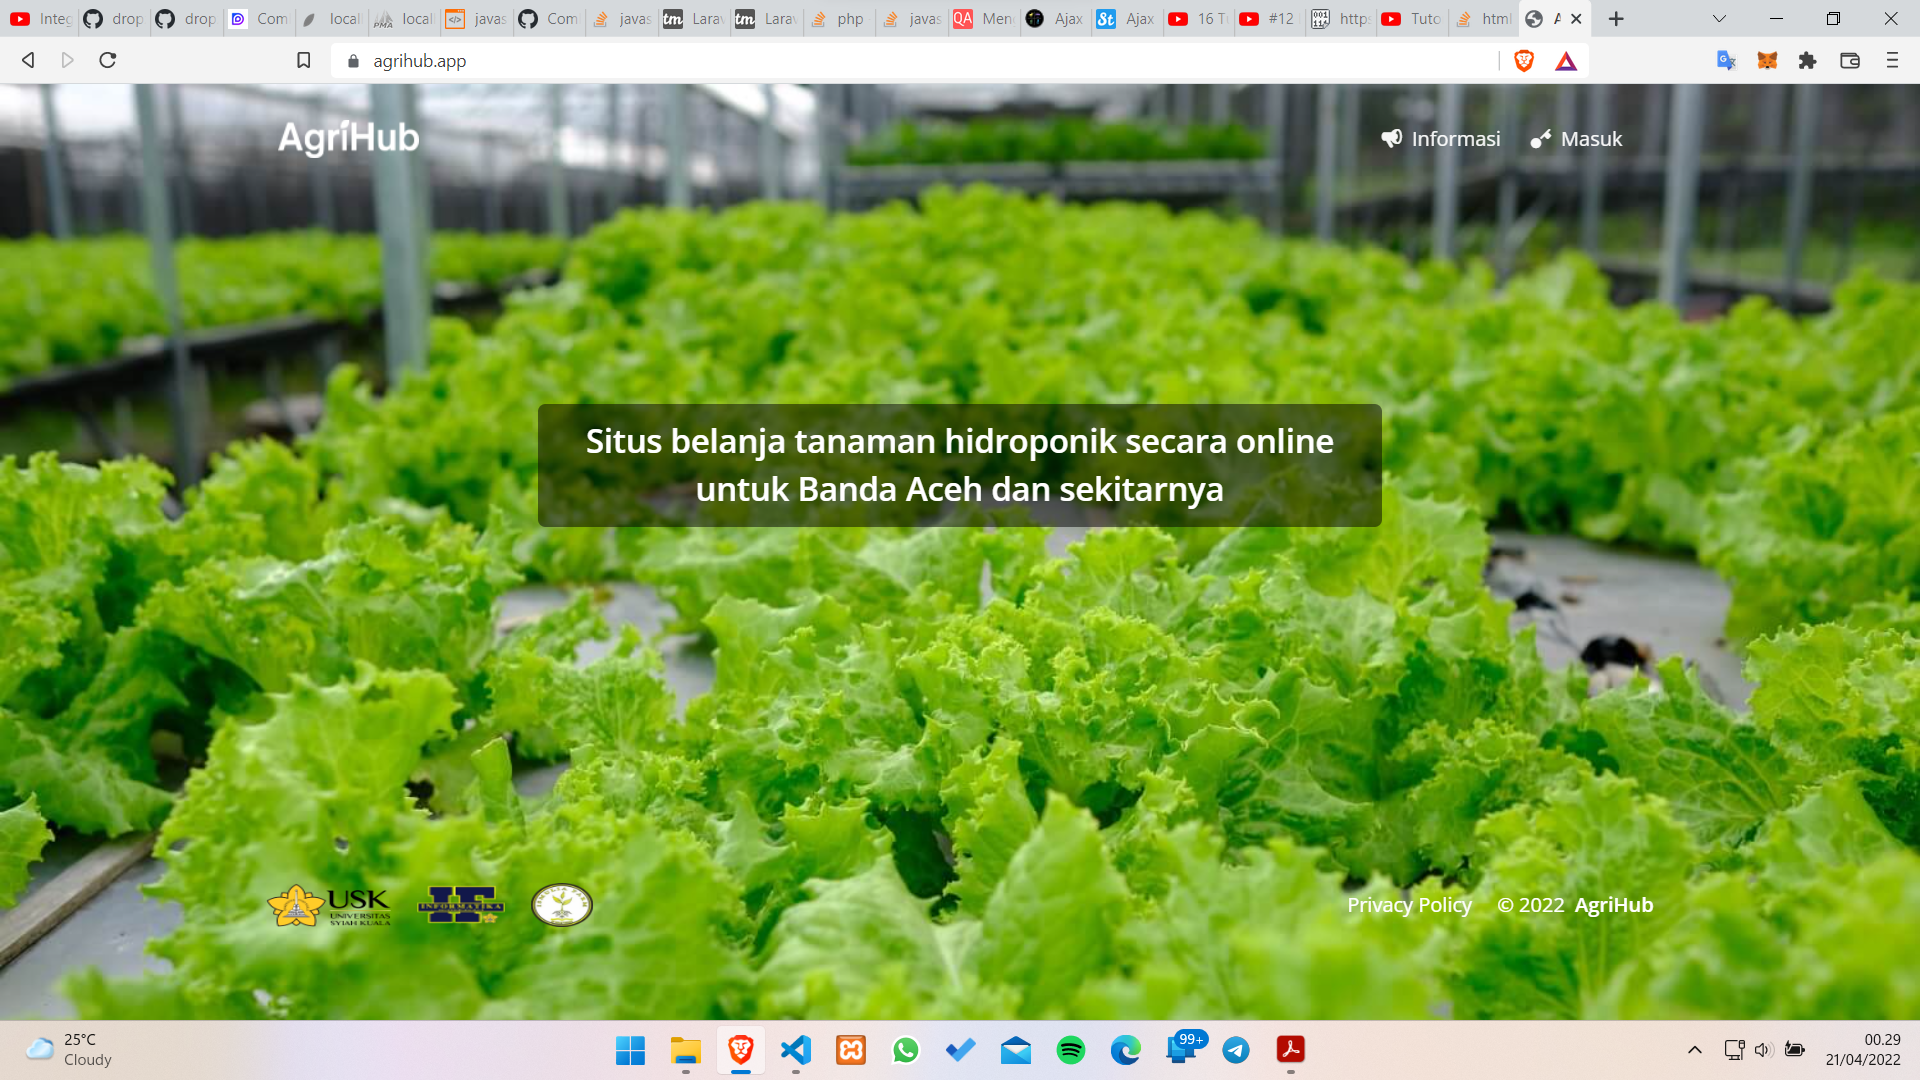
\includegraphics [width = 13.3cm, height= 8cm]{gambar/homepage}}
			\caption{Halaman Utama}
			\label{homepage}
		\end{figure}

		\item Halaman Masuk
		\par Halaman masuk merupakan halaman yang berfungsi untuk masuk kedalam aplikasi dengan cara mengisi \textit{email} dan \textit{password} lalu menekan tombol Masuk yang berwarna hijau. Apabila data yang diisi benar, maka proses masuk akan berhasil. Halaman masuk dapat dilihat pada gambar \ref*{login}.
		\begin{figure}[H]
			\centering
			{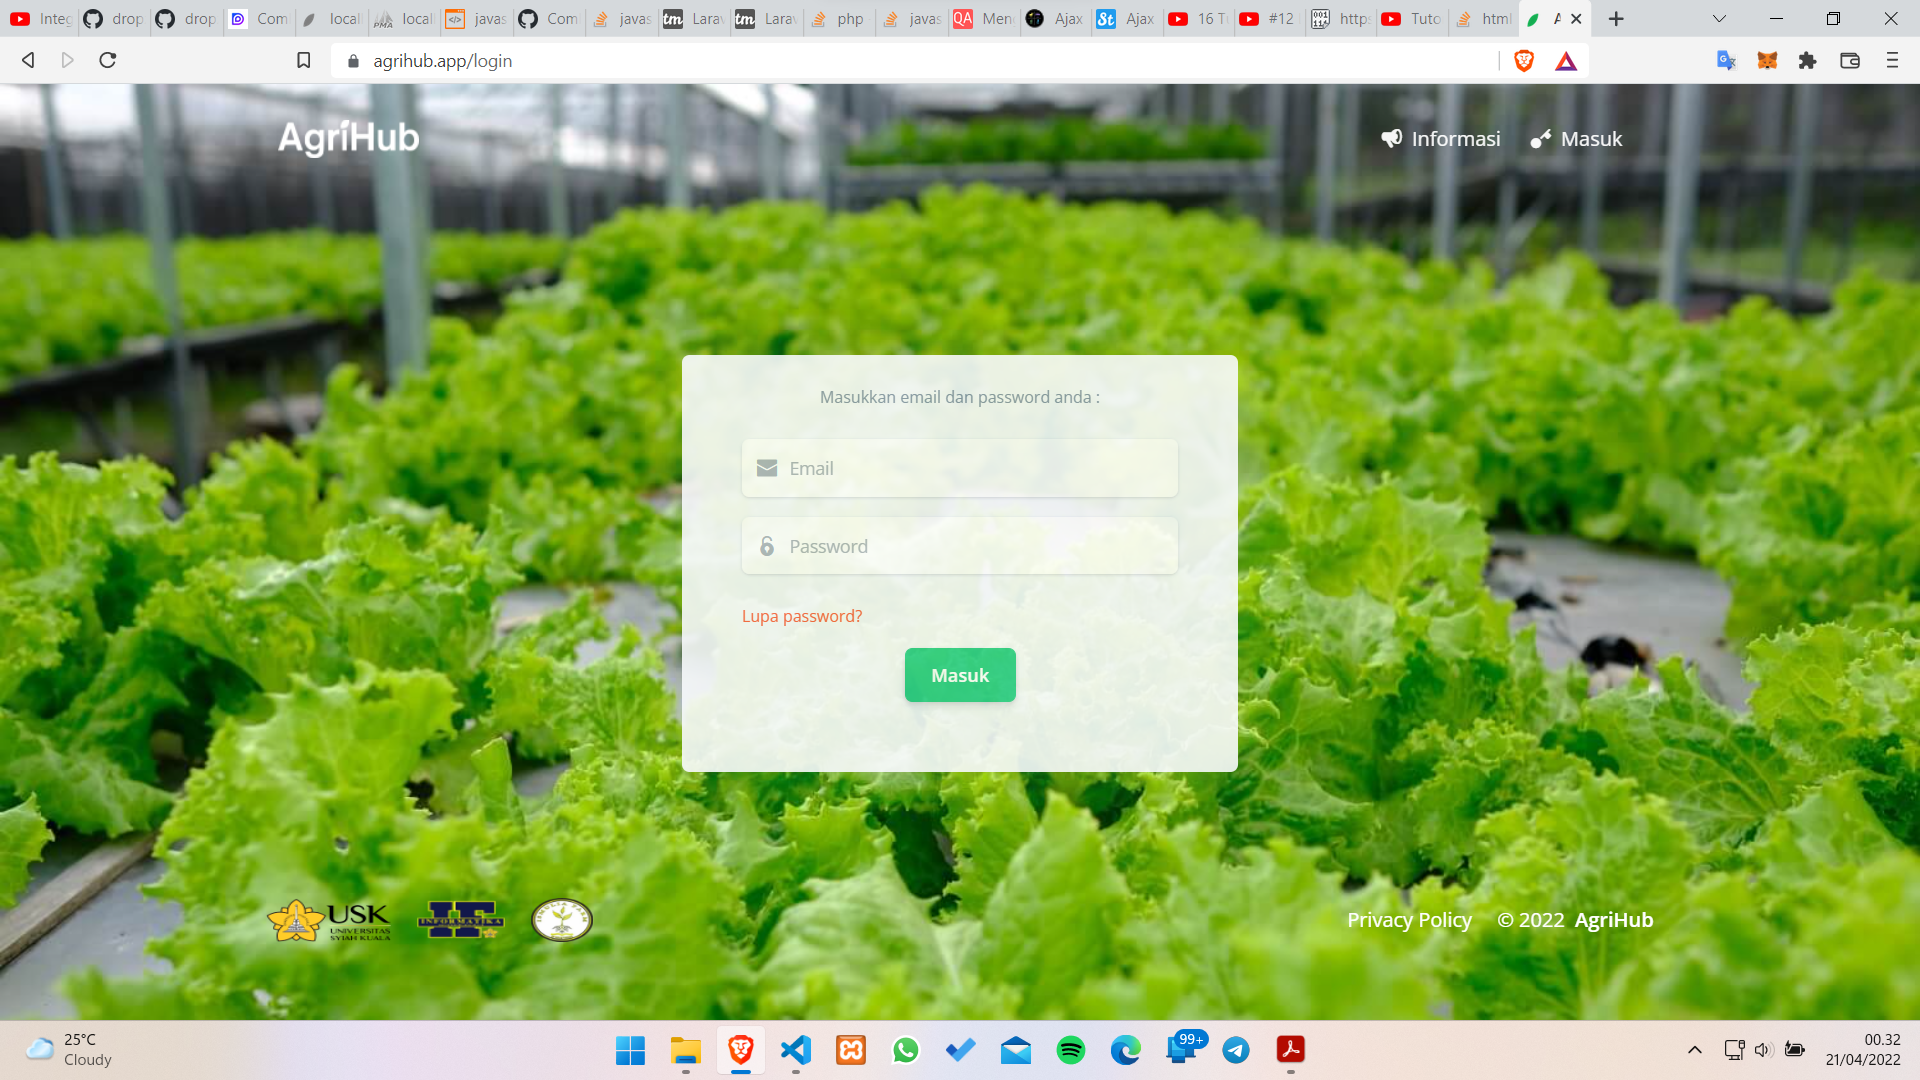
\includegraphics [width = 13.3cm, height= 8cm]{gambar/login}}
			\caption{Halaman Masuk}
			\label{login}
		\end{figure}
	
		\newpage
		\item Halaman Dasbor
		\par Setelah berhasil masuk ke aplikasi, maka akan tampil halaman dasbor. Halaman ini berisi informasi data jumlah produk yang sudah diunggah oleh para penjual, jumlah pesanan yang sudah terjadi di aplikasi, jumlah promo yang sedang berlangsung, jumlah pengguna yang sudah terdaftar di aplikasi, jumlah laporan yang masuk dari pembeli, dan jumlah ulasan yang sudah diberikan oleh pembeli terhadap produk yang dijual oleh penjual. Serta ditampilkan grafik jumlah pesanan yang selesai dan batal perbulannya dari para penjual, dan grafik jumlah produk baru yang diunggah oleh para penjual selama 6 bulan terakhir serta grafik jumlah admin, penjual dan pembeli. Halaman dasbor admin dapat dilihat pada gambar \ref*{dashboard_admin}.
		\begin{figure}[H]
			\centering
			{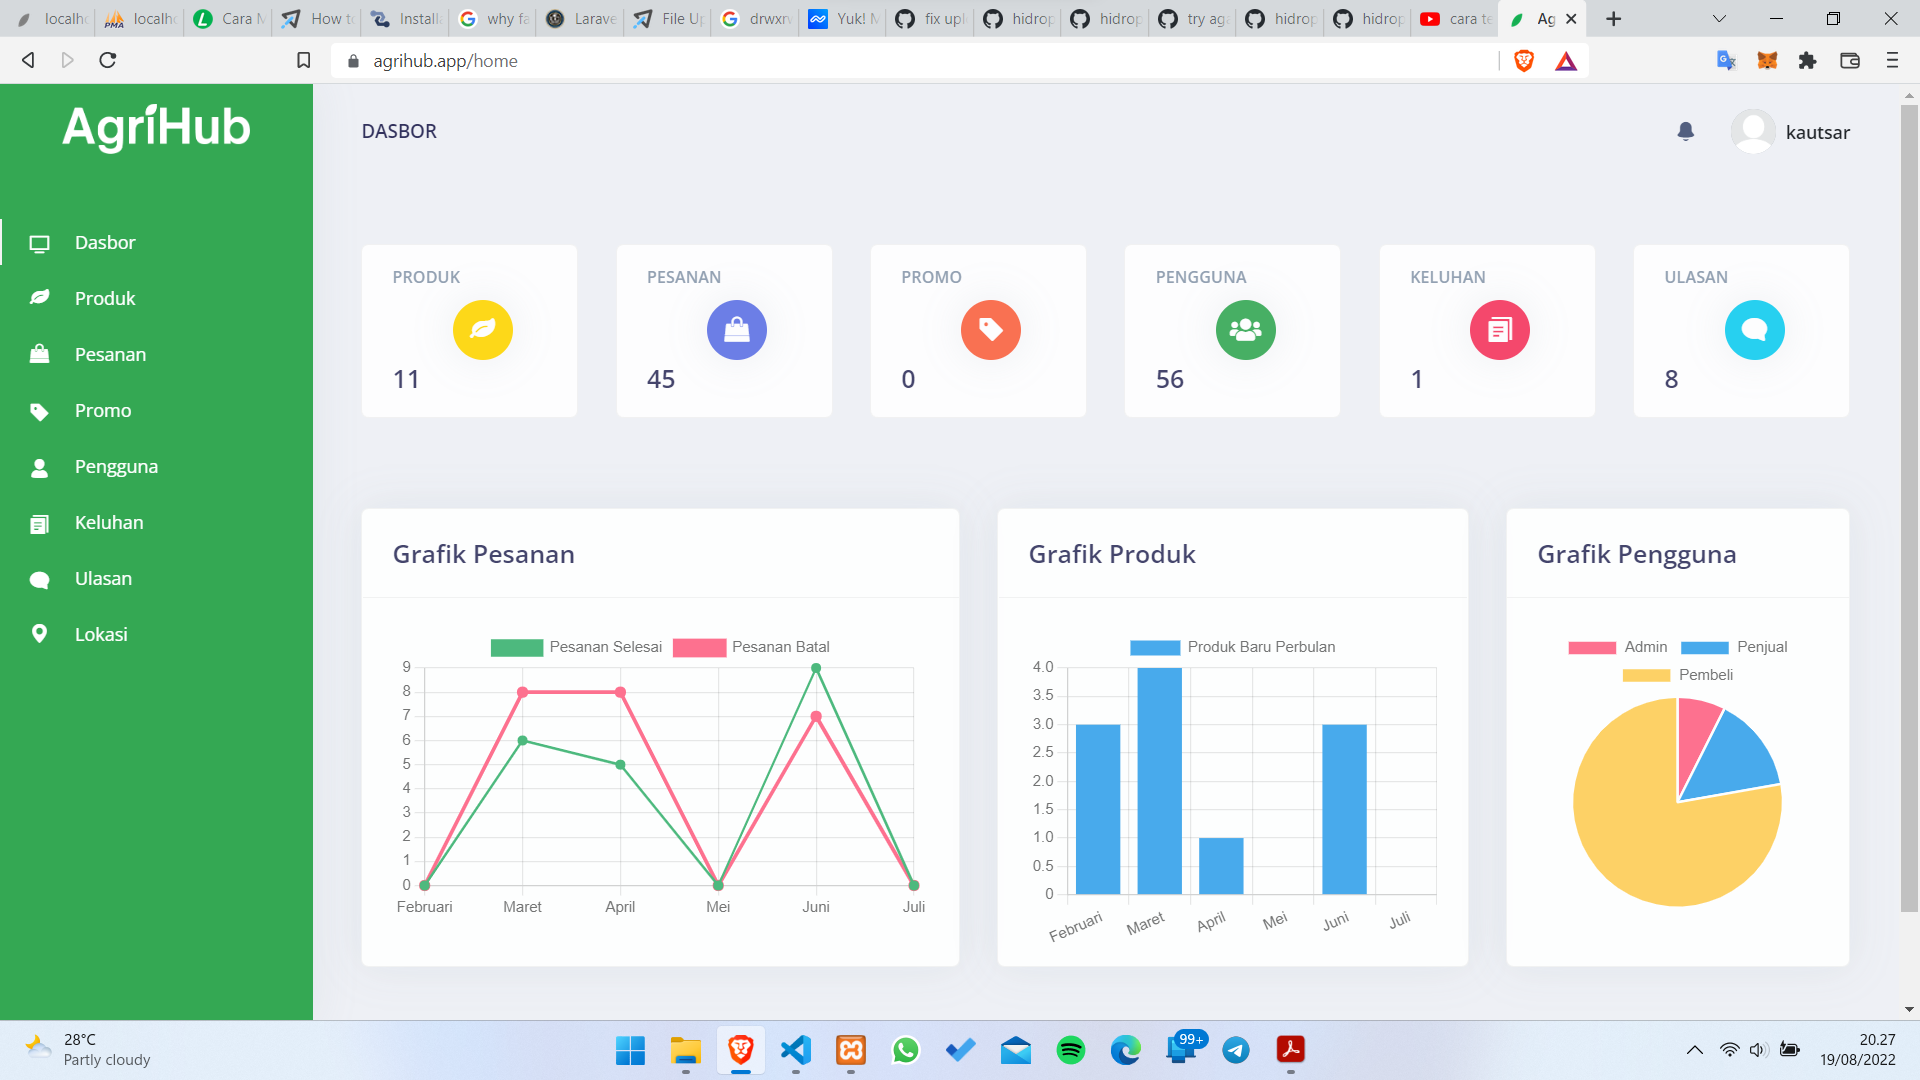
\includegraphics [width = 13.3cm, height= 8cm]{gambar/admin/dashboard_admin}}
			\caption{Halaman Dasbor pada sisi Admin}
			\label{dashboard_admin}
		\end{figure}

		\item Halaman Produk
		\par Pada halaman produk, admin dapat melihat informasi mengenai produk seperti id produk, gambar produk, nama produk dan lainnya. Admin juga dapat melakukan pencarian produk tertentu dengan memasukkan kata kunci di kolom cari produk, serta dapat menfilter produk berdasarkan satuannya dan menampilkan produk perhalaman sebanyak 5, 10, atau 25 data. Dikarenakan gambar produk bisa lebih dari 1 maka admin dapat melihat gambar produk lainnya beserta dengan keterangan produk dan jumlah/satuannya dengan menekan tombol Lihat. Admin juga dapat menghapus produk penjual jika diperlukan dengan menekan tombol Hapus. Halaman produk dan tampilan detail produk dapat dilihat pada gambar berikut ini.
		\begin{figure}[H]
			\centering
			{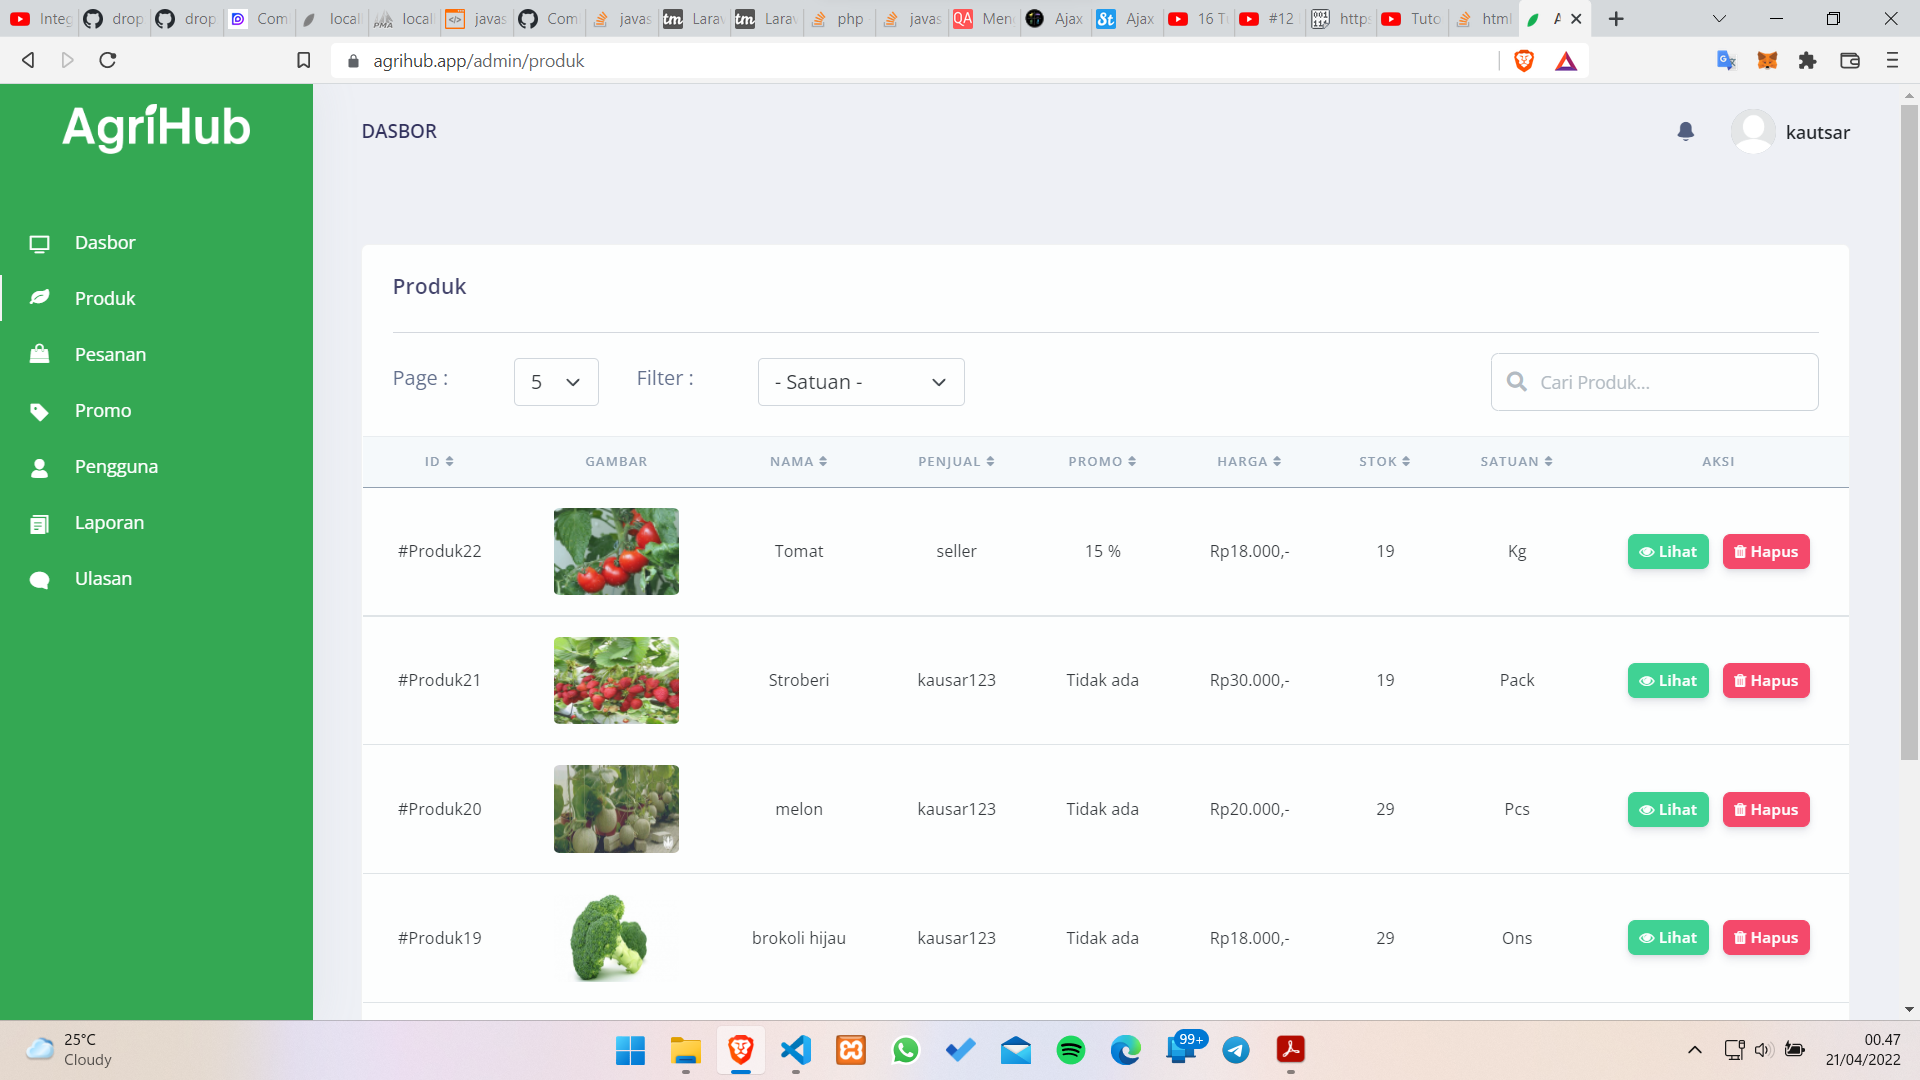
\includegraphics [width = 13.3cm, height= 8cm]{gambar/admin/produk_admin}}
			\caption{Halaman Produk pada sisi Admin}
			\label{produk_admin}
		\end{figure}
		\begin{figure}[H]
			\centering
			{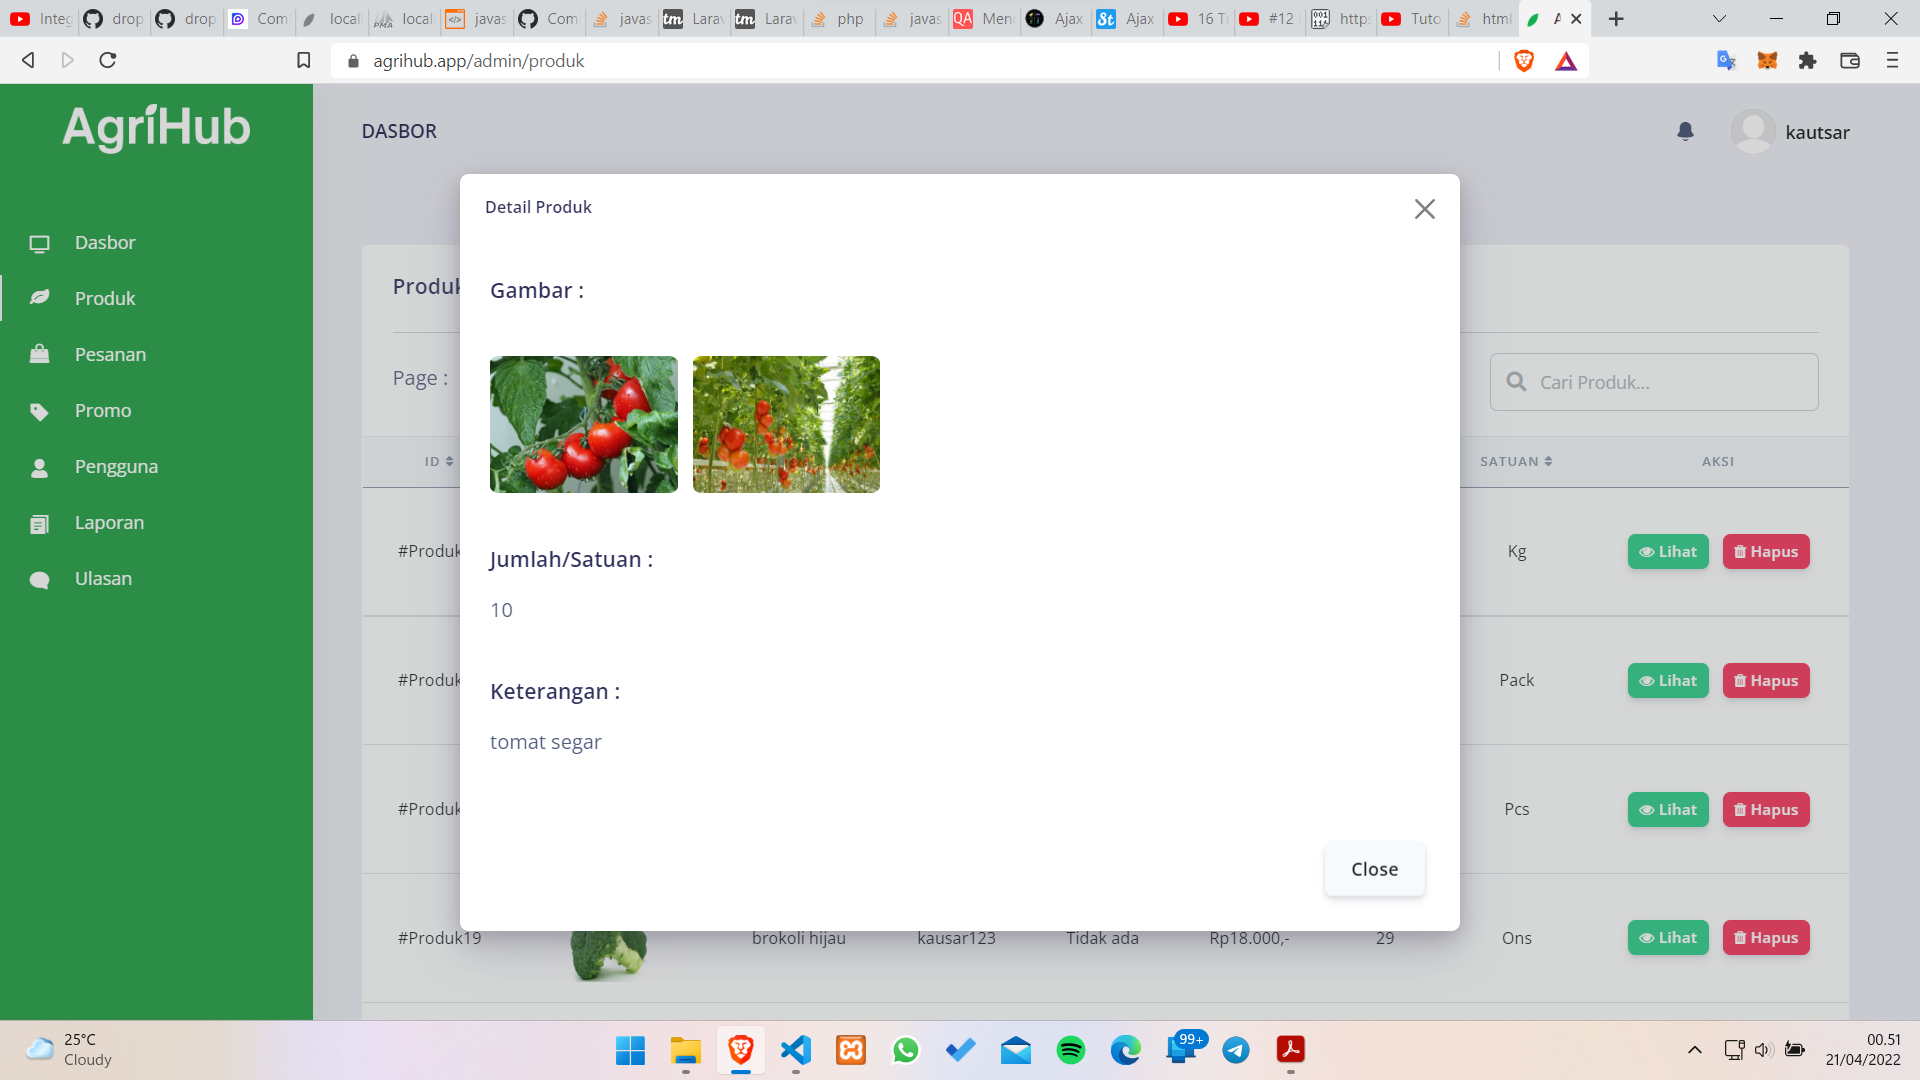
\includegraphics [width = 13.3cm, height= 8cm]{gambar/admin/lihat_produk_admin}}
			\caption{Tampilan Detail Produk}
			\label{lihat_produk_admin}
		\end{figure}

		\item Halaman Pesanan
		\par Pada halaman pesanan admin dapat melihat semua pesanan yang sudah terjadi diaplikasi antara penjual dengan pembeli, dan dapat menfilter datanya berdasarkan status pesanannya. Admin juga dapat melihat detail pesanan dengan menekan tombol Detail serta dapat mengekspor datanya dalam bentuk pdf jika diperlukan dengan menekan tombol \textit{Export} PDF. Halaman pesanan dan tampilan detail serta ekspor pdf pesanan dapat dilihat pada gambar berikut ini.
		\begin{figure}[H]
			\centering
			{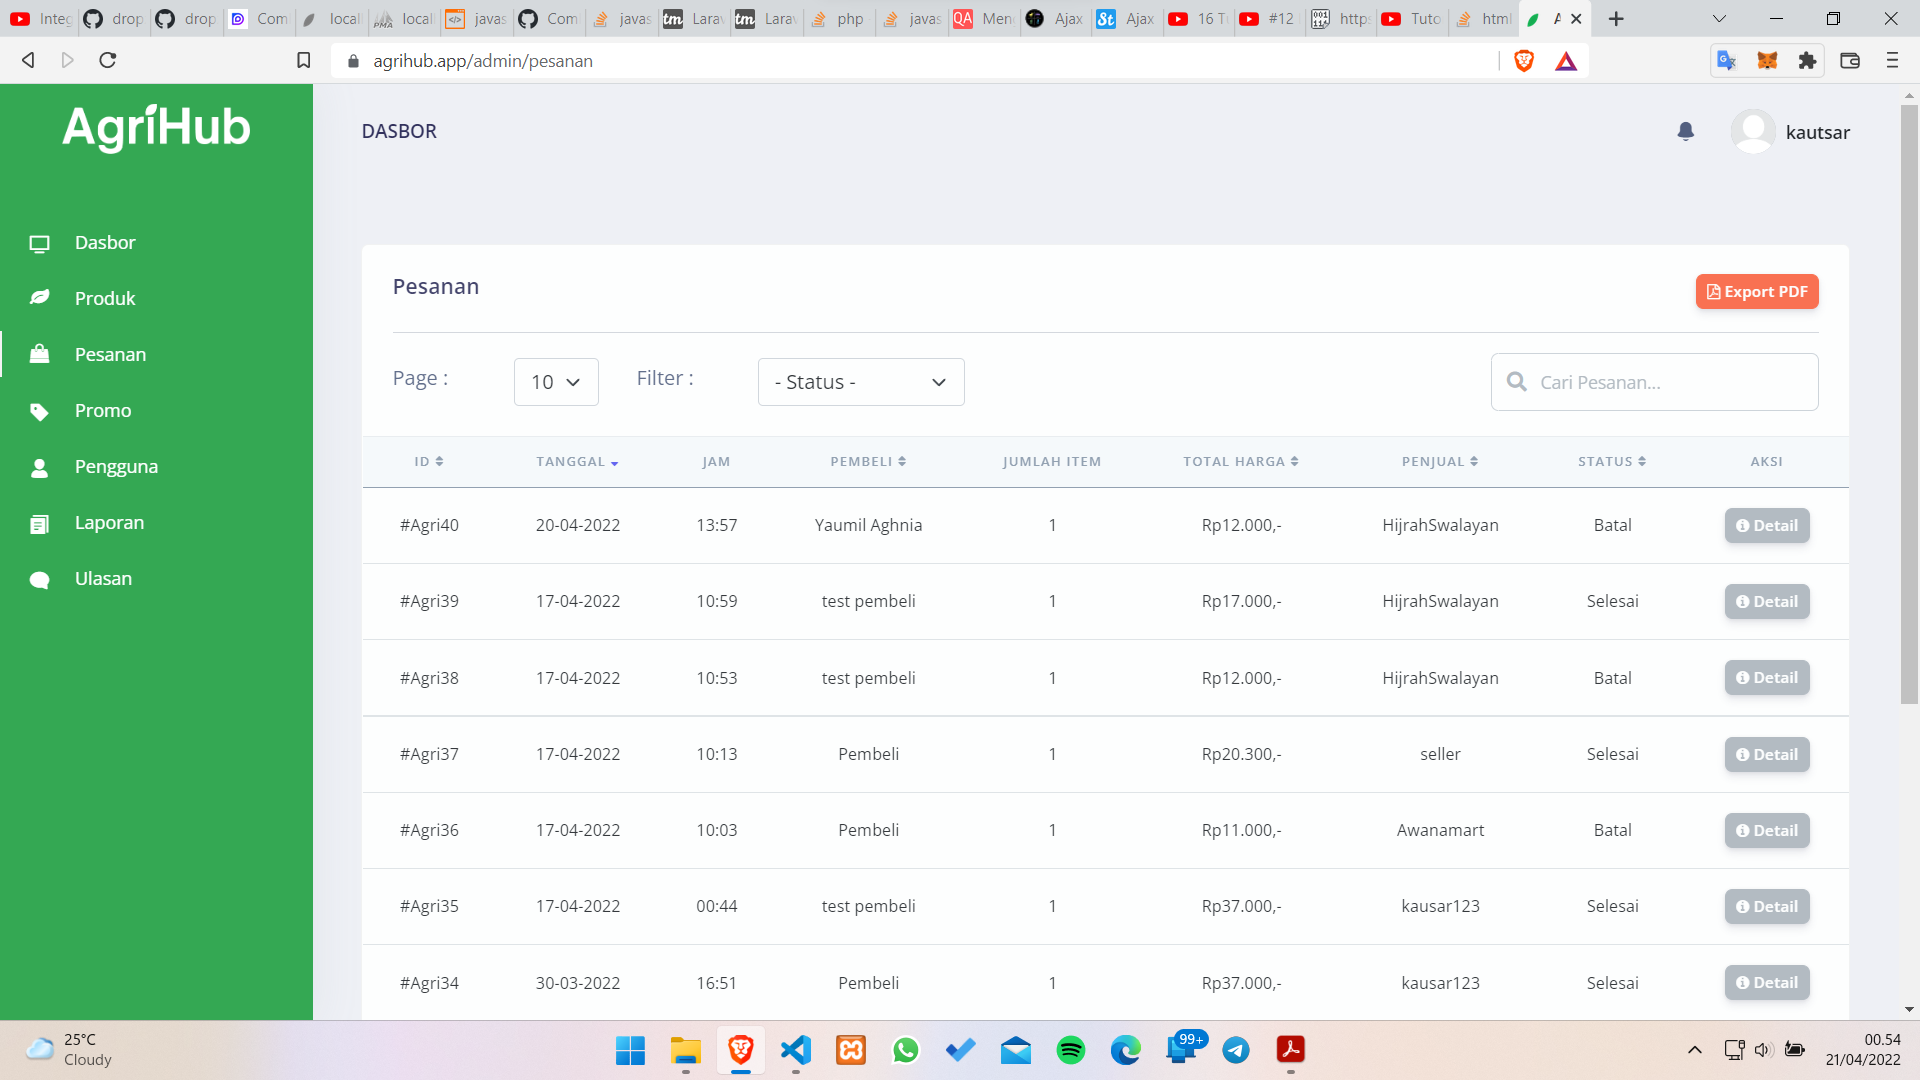
\includegraphics [width = 13.3cm, height= 8cm]{gambar/admin/pesanan_admin}}
			\caption{Halaman Pesanan pada sisi Admin}
			\label{pesanan_admin}
		\end{figure}
		\begin{figure}[H]
			\centering
			{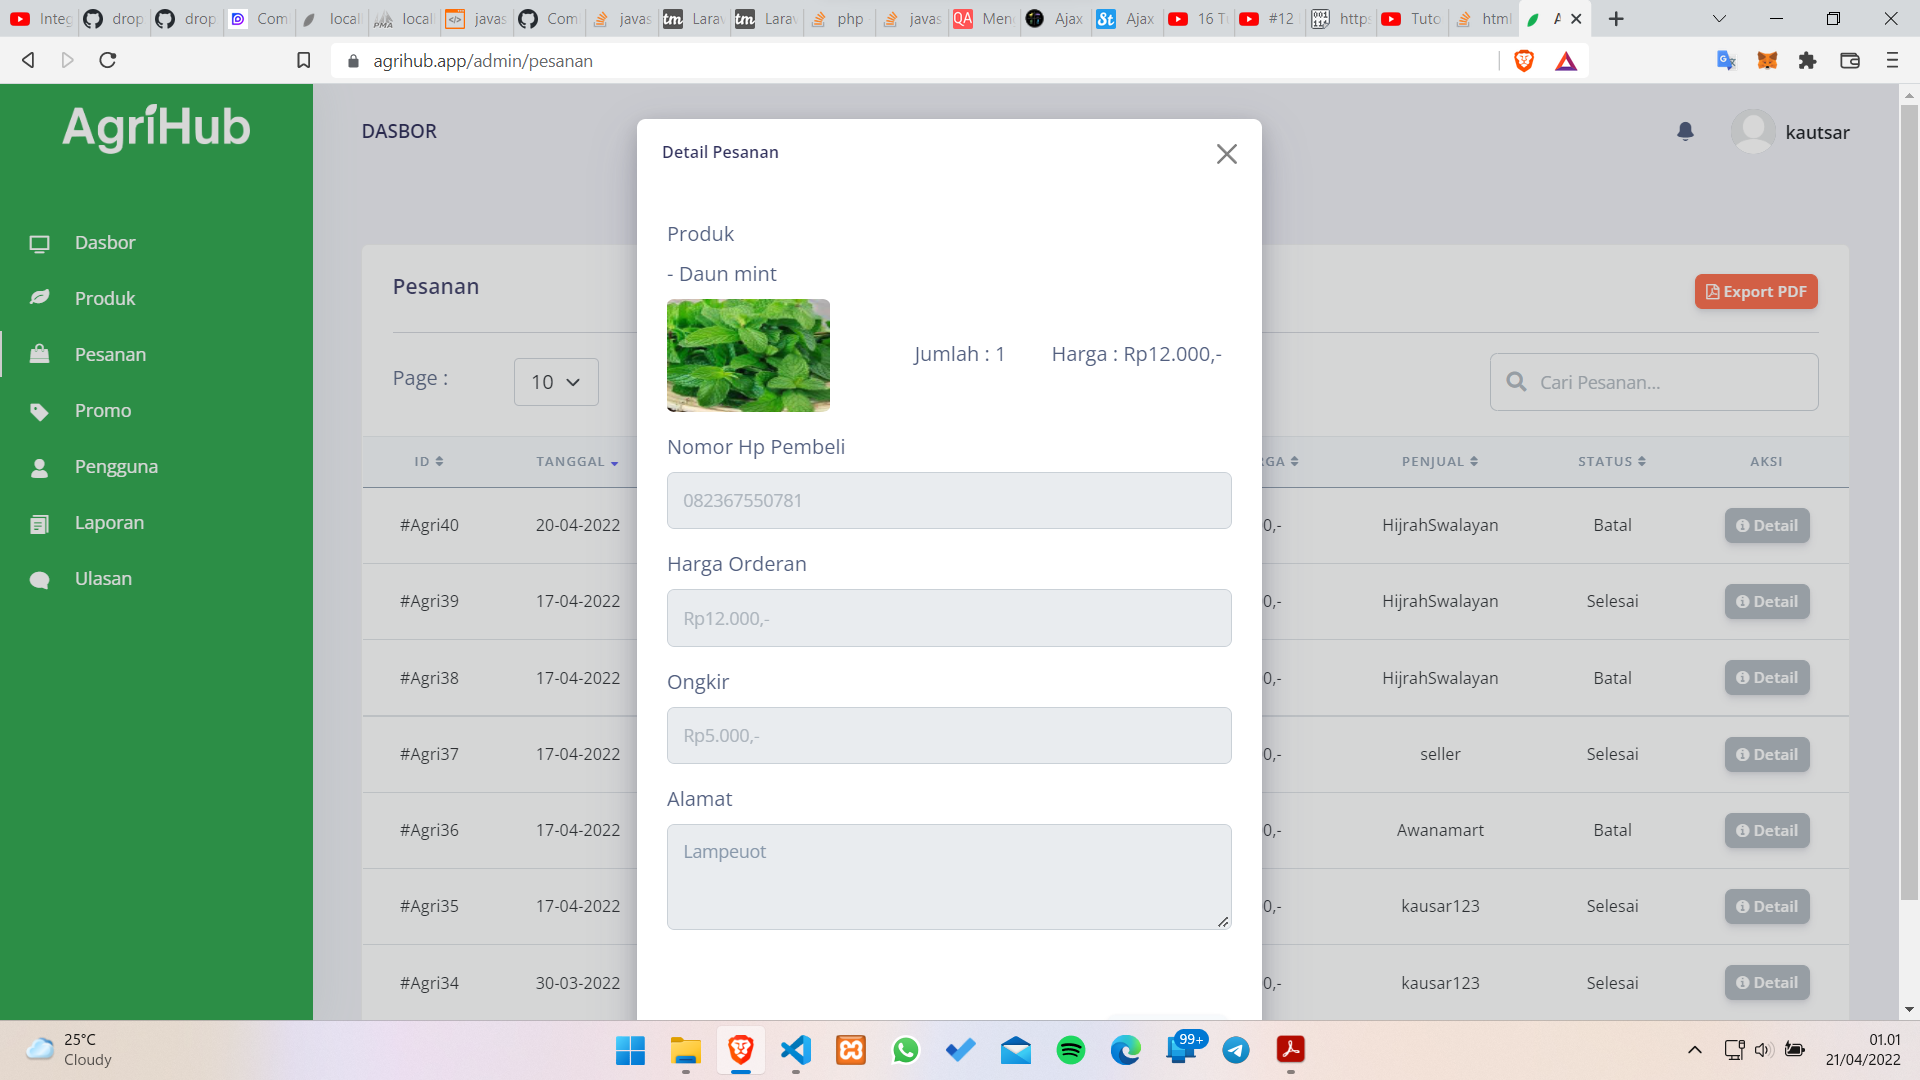
\includegraphics [width = 13.3cm, height= 8cm]{gambar/admin/detail_pesanan}}
			\caption{Tampilan Detail Pesanan}
			\label{detail_pesanan}
		\end{figure}
		\begin{figure}[H]
			\centering
			{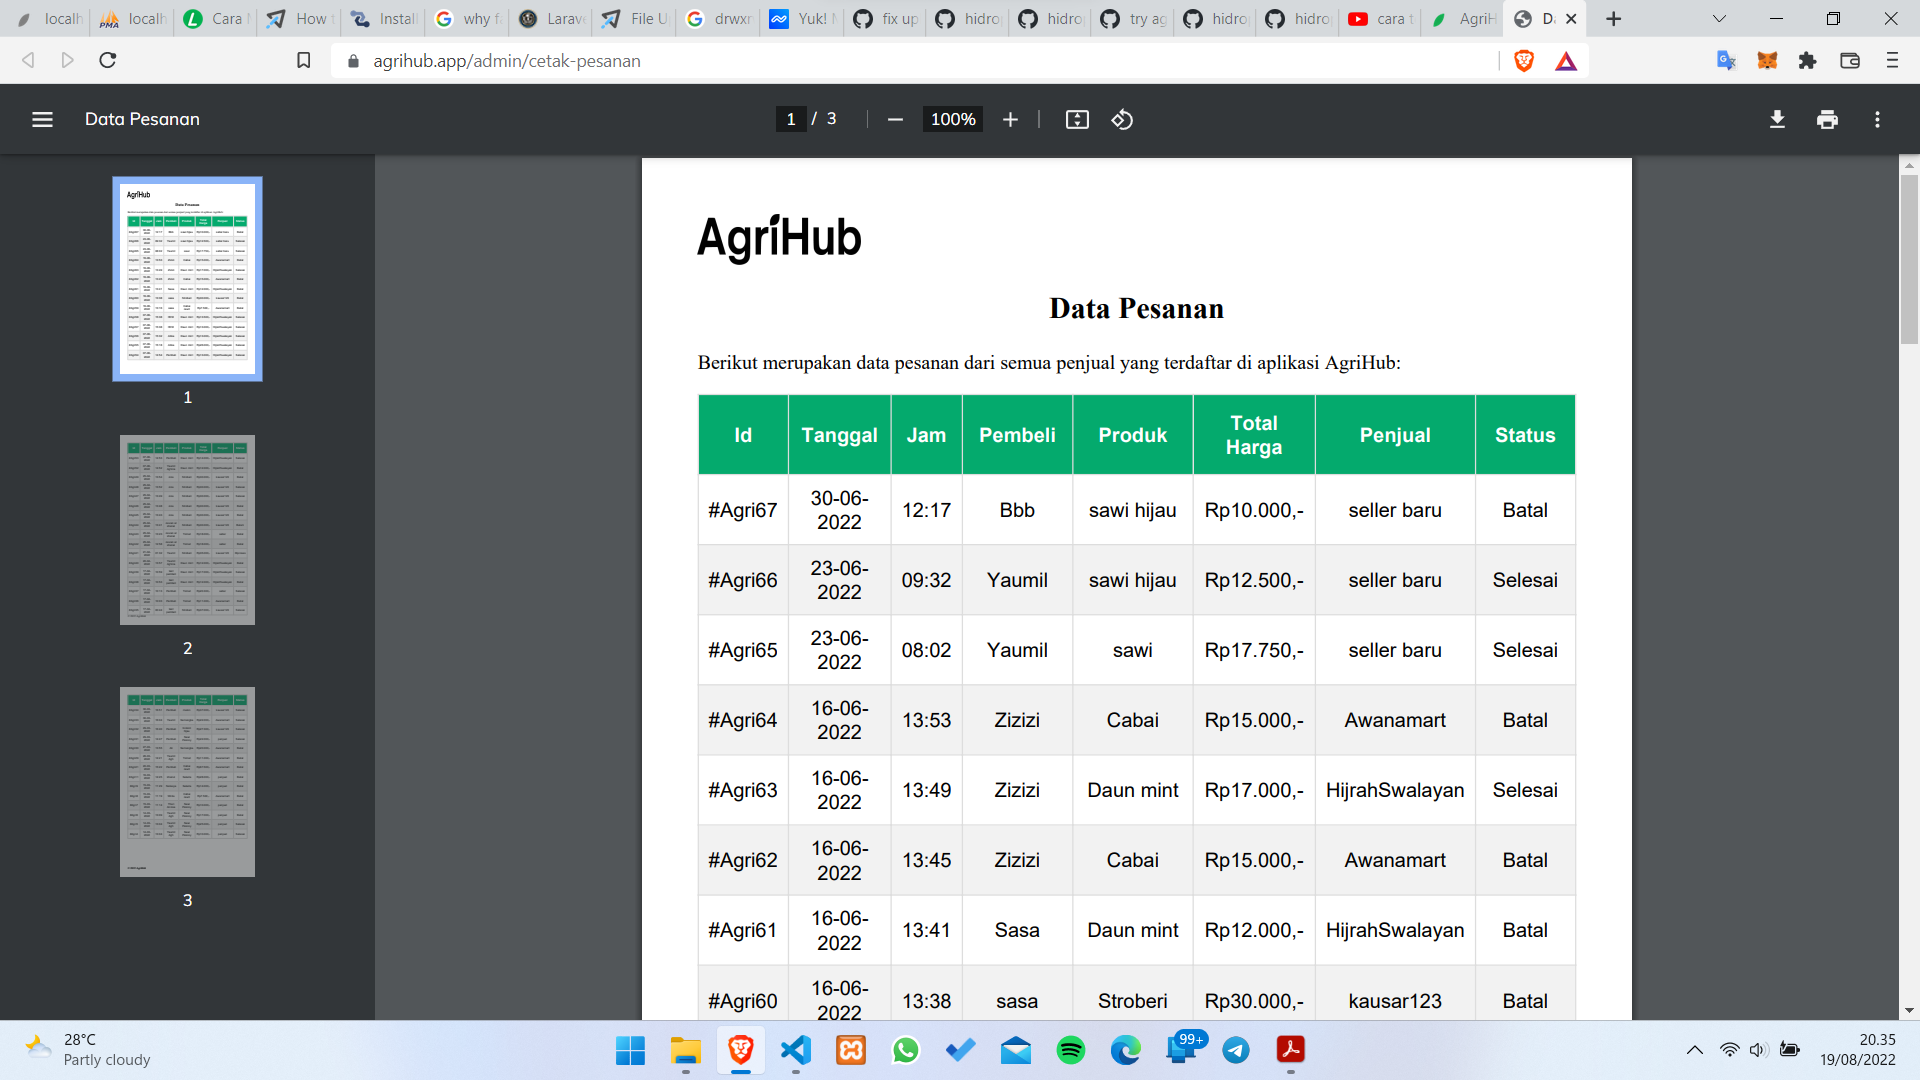
\includegraphics [width = 13.3cm, height= 8cm]{gambar/admin/export_pesanan_admin}}
			\caption{Tampilan Ekspor PDF Pesanan pada sisi Admin}
			\label{export_pesanan_admin}
		\end{figure}

		\item Halaman Promo
		\par Pada halaman ini admin dapat mengelola promo seperti menambahkan promo baru kedalam aplikasi sehingga nantinya dapat digunakan oleh para penjual, dan dapat juga mengubah data promo yang sudah ada atau menghapusnya. Halaman promo dan tampilan tambah serta ubah promo dapat dilihat pada gambar dibawah ini.
		\begin{figure}[H]
			\centering
			{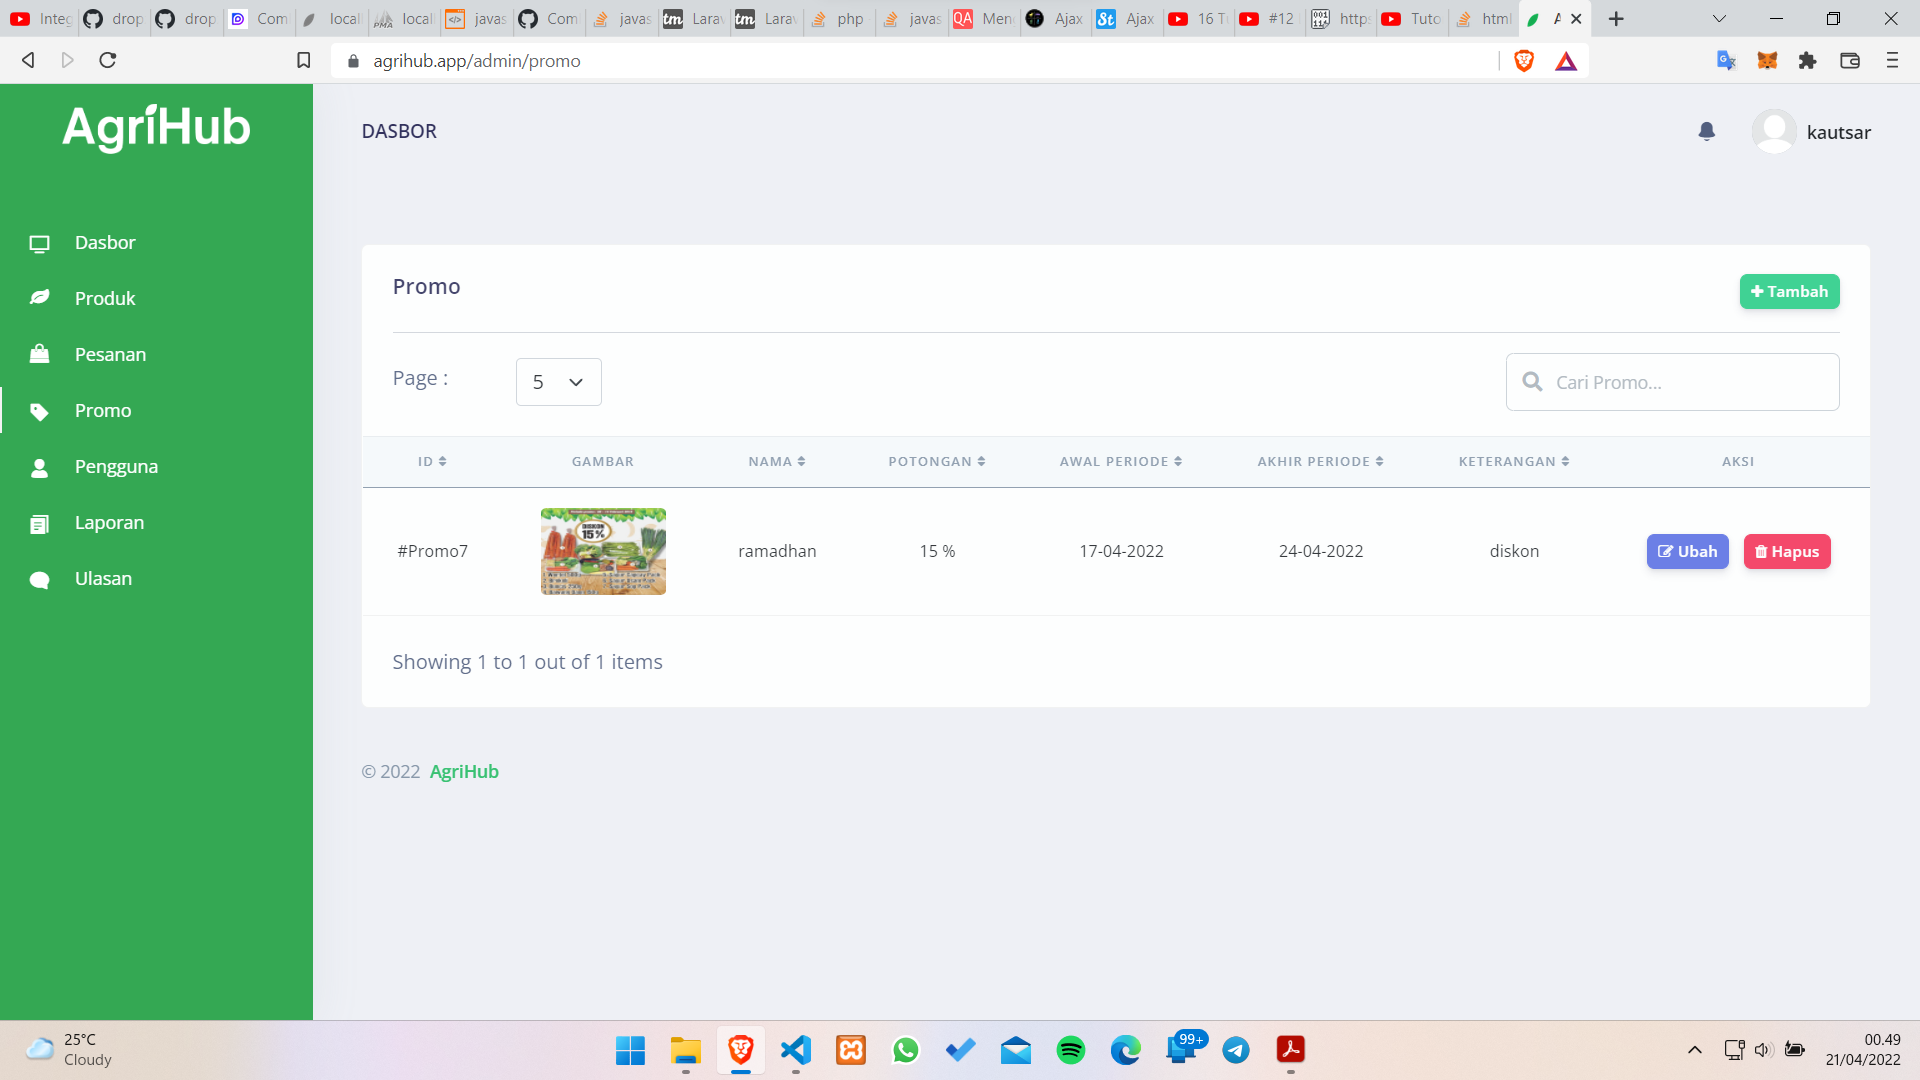
\includegraphics [width = 13.3cm, height= 8cm]{gambar/admin/promo}}
			\caption{Halaman Promo}
			\label{promo}
		\end{figure}
		\begin{figure}[H]
			\centering
			{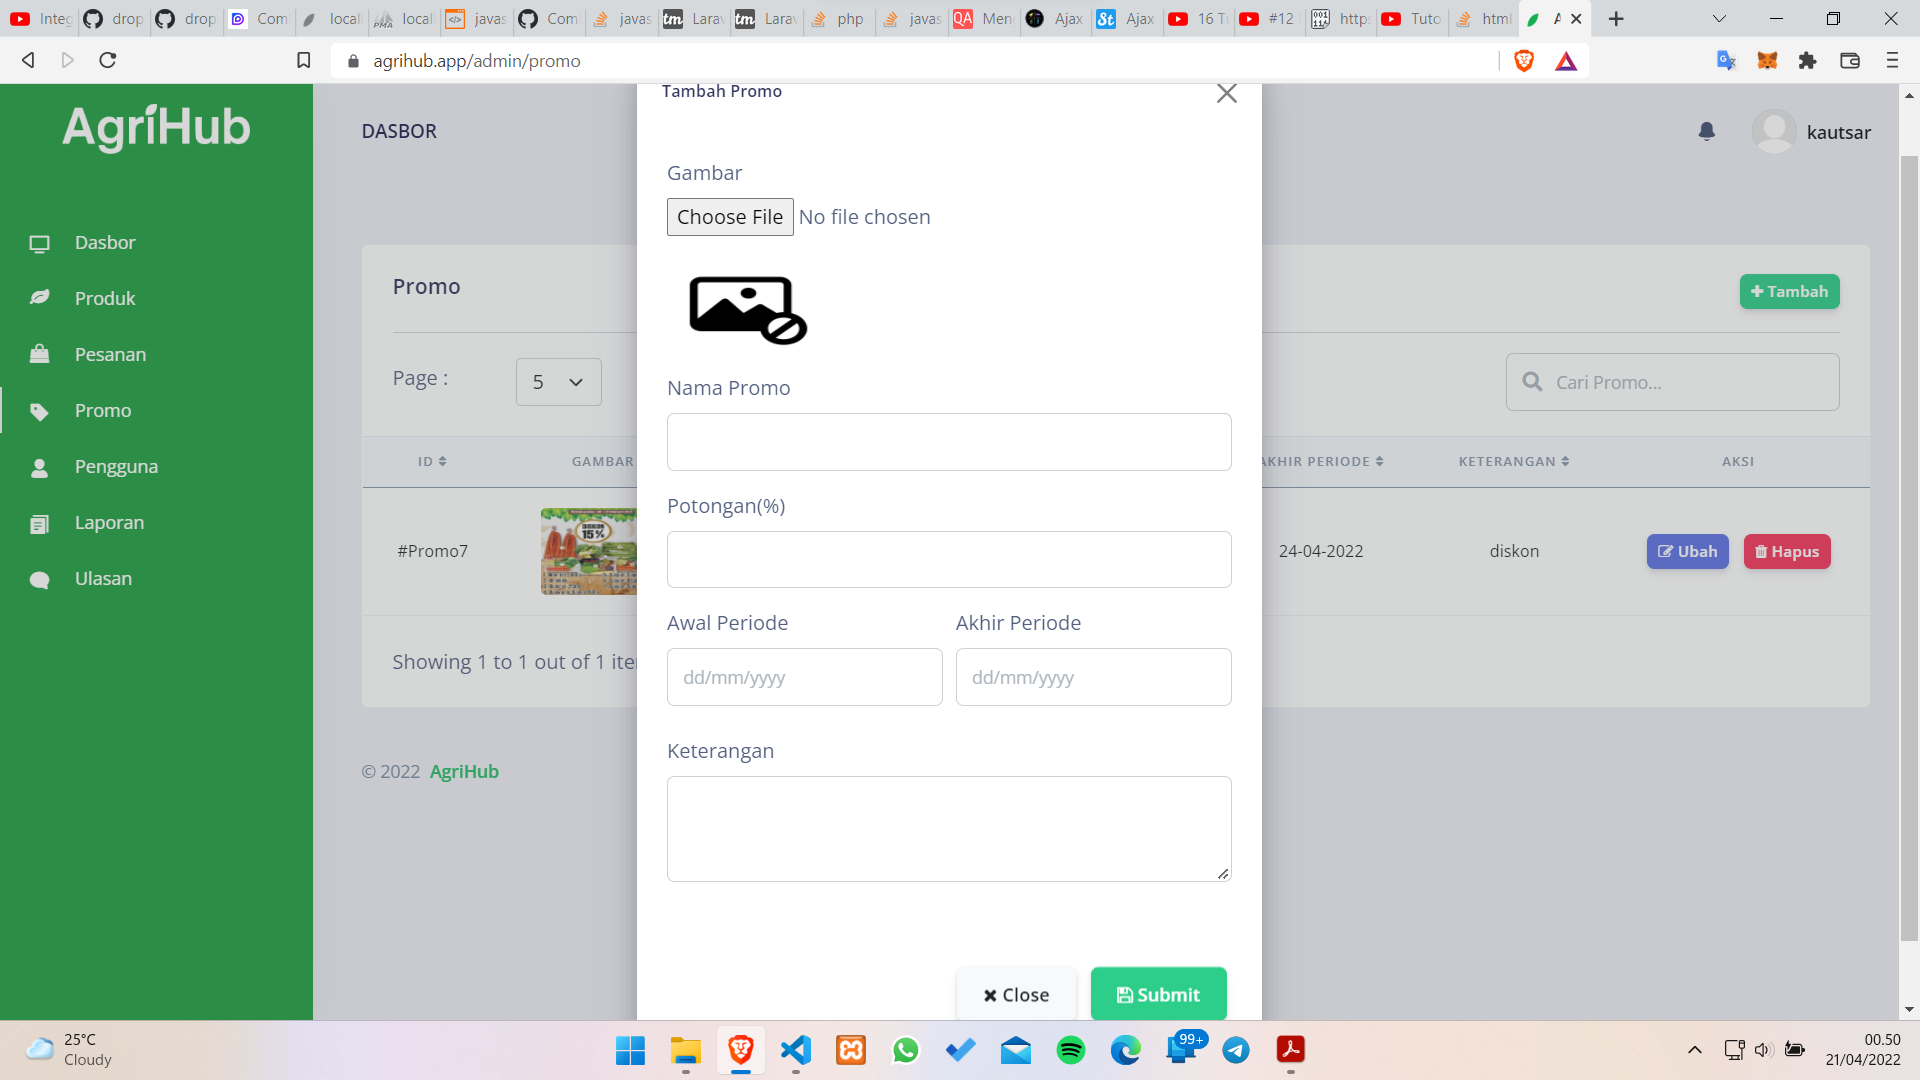
\includegraphics [width = 13.3cm, height= 8cm]{gambar/admin/tambah_promo}}
			\caption{Tampilan Tambah Promo}
			\label{tambah_promo}
		\end{figure}
		\begin{figure}[H]
			\centering
			{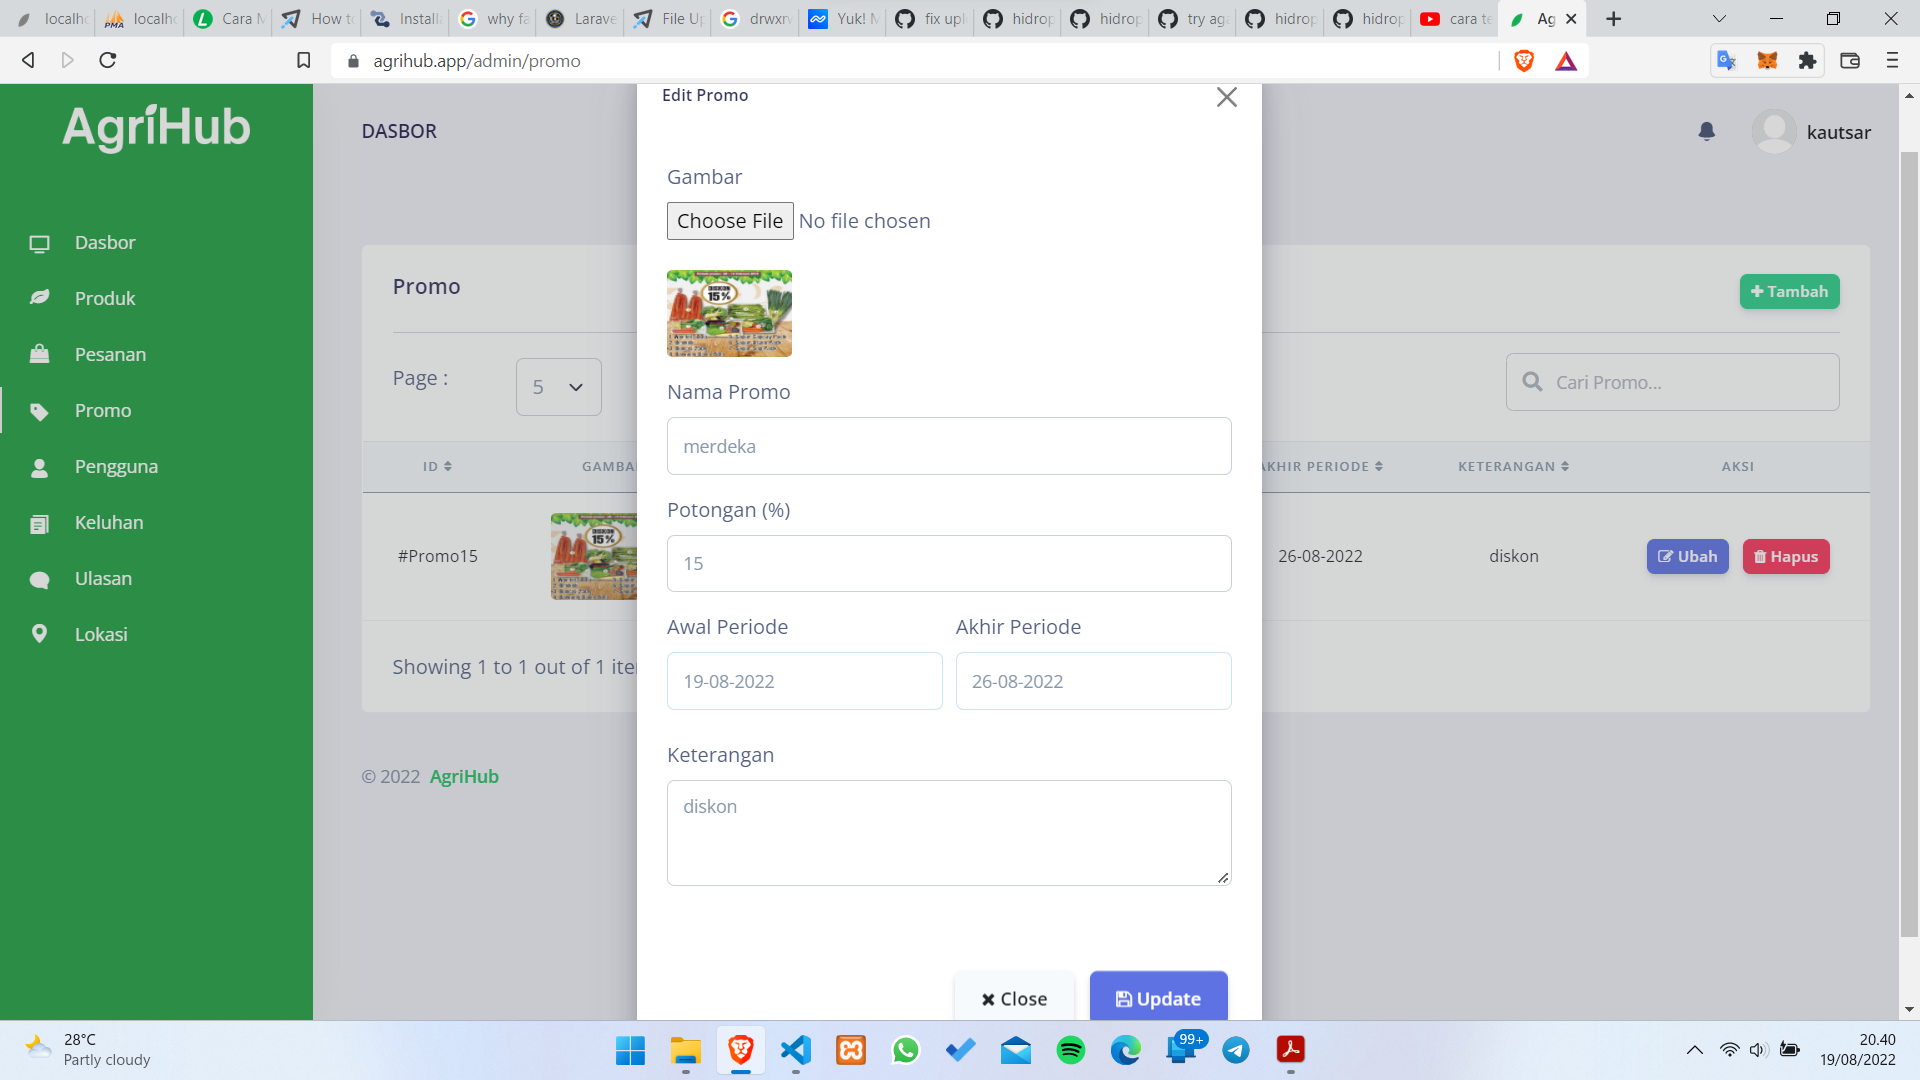
\includegraphics [width = 13.3cm, height= 8cm]{gambar/admin/ubah_promo}}
			\caption{Tampilan Ubah Promo}
			\label{ubah_promo}
		\end{figure}

		\item Halaman Pengguna
		\par Pada halaman pengguna ini admin data melihat semua data pengguna yang sudah terdaftar diaplikasi AgriHub ini baik itu admin, penjual maupun pembeli, serta dapat memblokir penjual atau pembeli yang melanggar. Juga dapat menambahkan akun penjual baru dengan menekan tombol tambah penjual dan mengisi data penjual. Halaman pengguna dan tampilan tambah akun penjual dapat dilihat pada gambar berikut ini.
		\begin{figure}[H]
			\centering
			{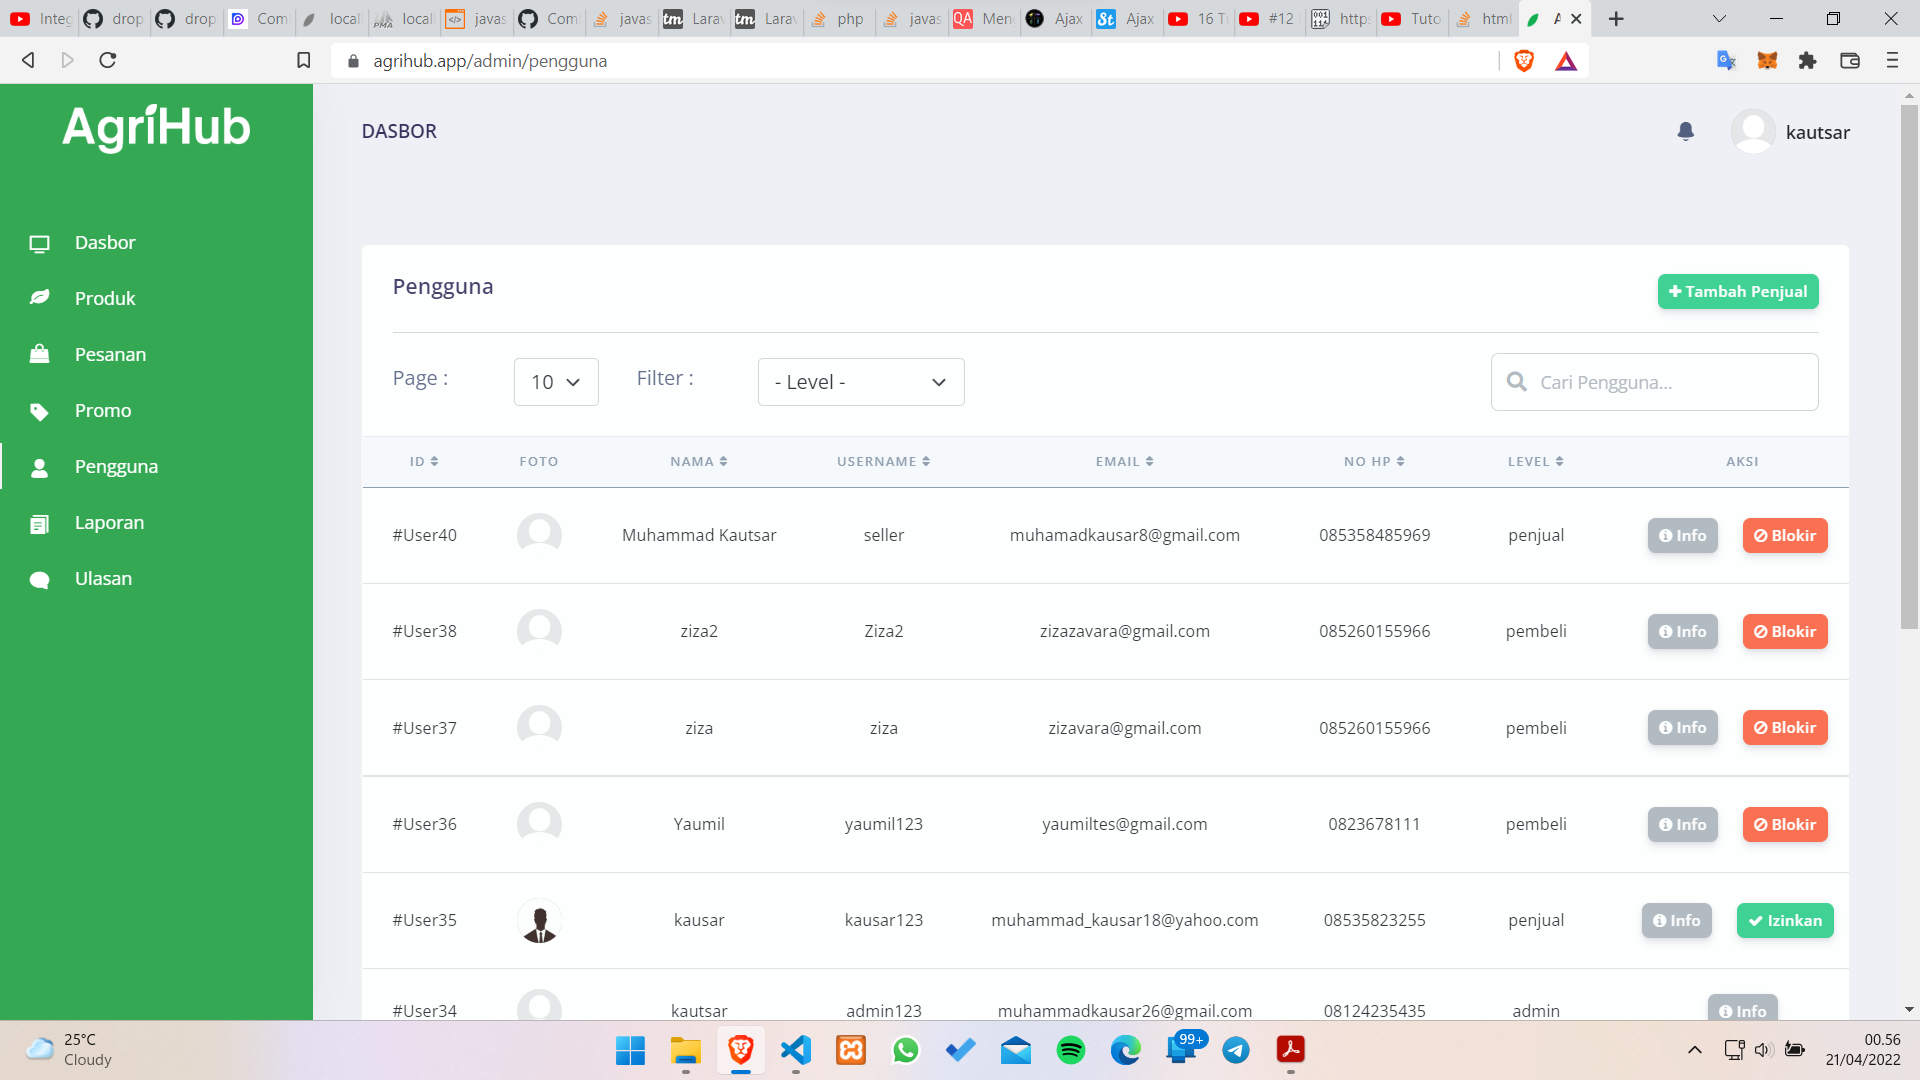
\includegraphics [width = 13.3cm, height= 8cm]{gambar/admin/pengguna}}
			\caption{Halaman Pengguna}
			\label{pengguna}
		\end{figure}
		\begin{figure}[H]
			\centering
			{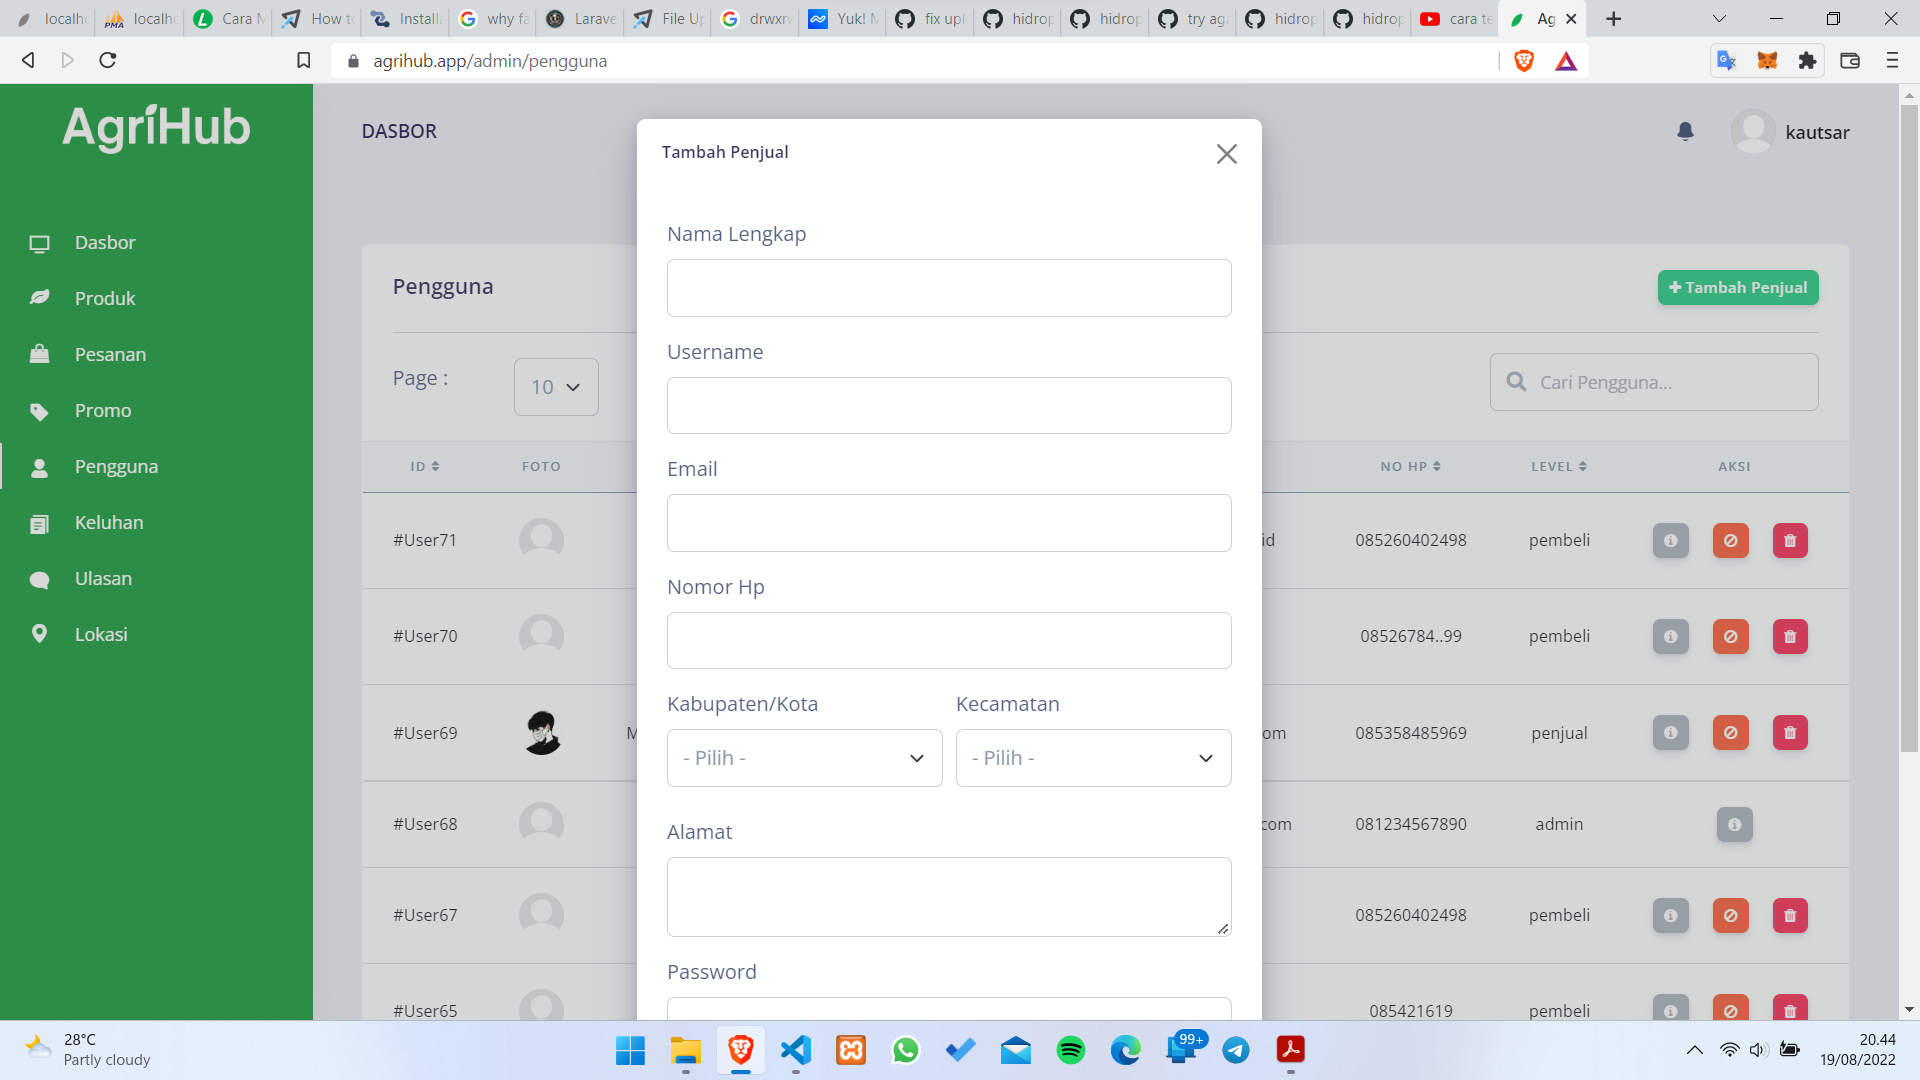
\includegraphics [width = 13.3cm, height= 8cm]{gambar/admin/tambah_pengguna}}
			\caption{Tampilan Tambah Akun Pejual}
			\label{tambah_pengguna}
		\end{figure}

		\item Halaman Laporan
		\par Pada halaman ini admin dapat melihat data laporan yang masuk dari para pembeli terhadap penjual seperti id, tanggal, isi laporan, nama pelapor dan nama penjual yang dilaporkan. Setelah mendapat laporan dari pembeli, admin dapat mengambil tindakan pemblokiran pada akun penjual tersebut melalui halaman pengguna. Halaman laporan dapat dilihat pada gambar \ref*{laporan}.
		\begin{figure}[H]
			\centering
			{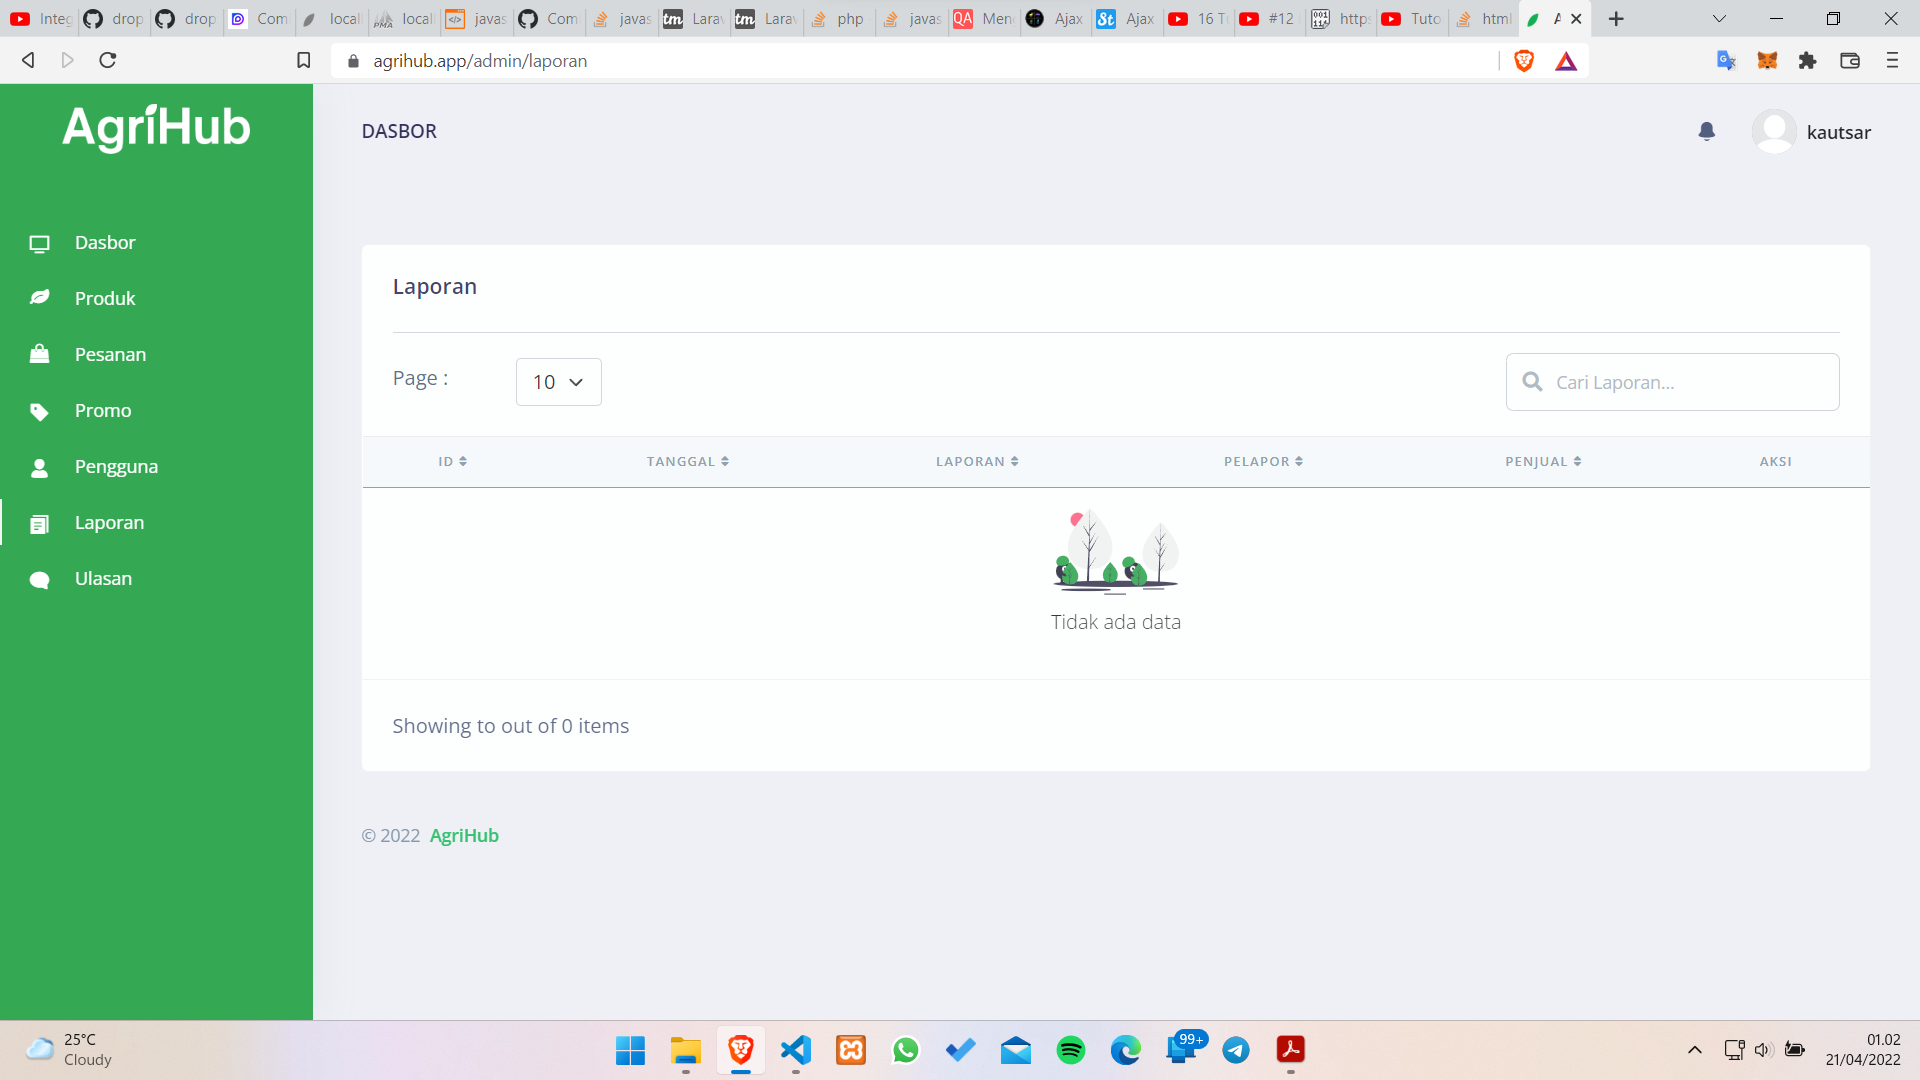
\includegraphics [width = 13.3cm, height= 8cm]{gambar/admin/laporan}}
			\caption{Halaman Laporan}
			\label{laporan}
		\end{figure}

		\item Halaman Ulasan
		\par Halaman ulasan berisi semua ulasan yang sudah diberikan oleh para pembeli terhadap produk yang dia beli dari penjual. Admin dapat menfilter ulasannya berdasarkan rating bintang yang diberikan oleh pembeli dan dapat juga menghapus ulasan pembeli jika dianggap mengandung kata tidak pantas. Halaman ulasan dapat dilihat pada gambar \ref*{ulasan_admin}.
		\begin{figure}[H]
			\centering
			{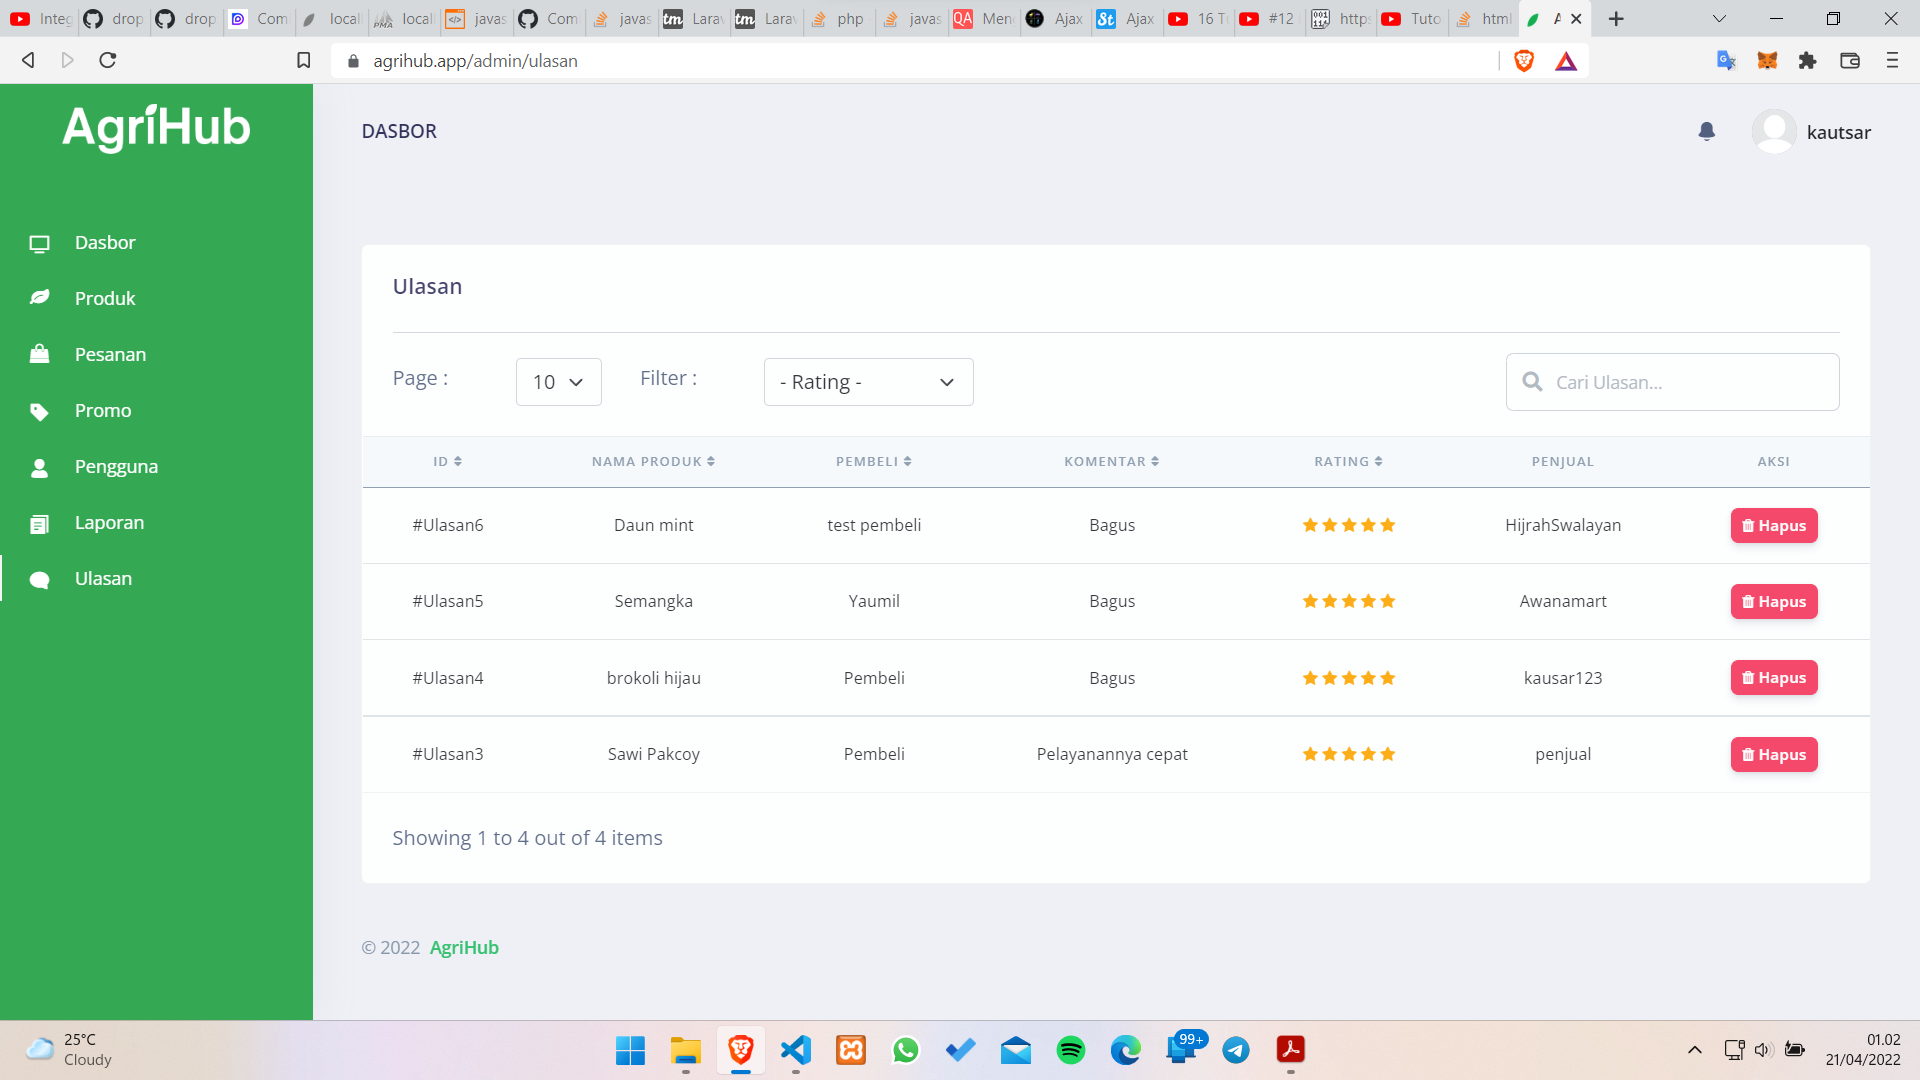
\includegraphics [width = 13.3cm, height= 8cm]{gambar/admin/ulasan_admin}}
			\caption{Halaman Ulasan pada sisi Admin}
			\label{ulasan_admin}
		\end{figure}
	\end{enumerate}

	\newpage
	\item Antarmuka Aplikasi Bagian Penjual
	\par Antarmuka aplikasi pada bagian penjual pada dasarnya hampir sama seperti antarmuka pada bagian admin hanya saja ada beberapa halaman dan menunya yang berbeda. Halaman aplikasi pada bagian penjual sebagai berikut :

	\begin{enumerate}[a.]
		\item Halaman Informasi
		\par Halaman informasi menampilkan informasi mengenai tata cara mendaftar sebagai penjual diaplikasi AgriHub ini. Penjual dapat mengakses halaman informasi ini dengan menklik \textit{tab} informasi yang ada dipojok kanan atas pada halaman utama. Halaman informasi dapat dilihat pada gambar \ref*{informasi}.
		\begin{figure}[H]
			\centering
			{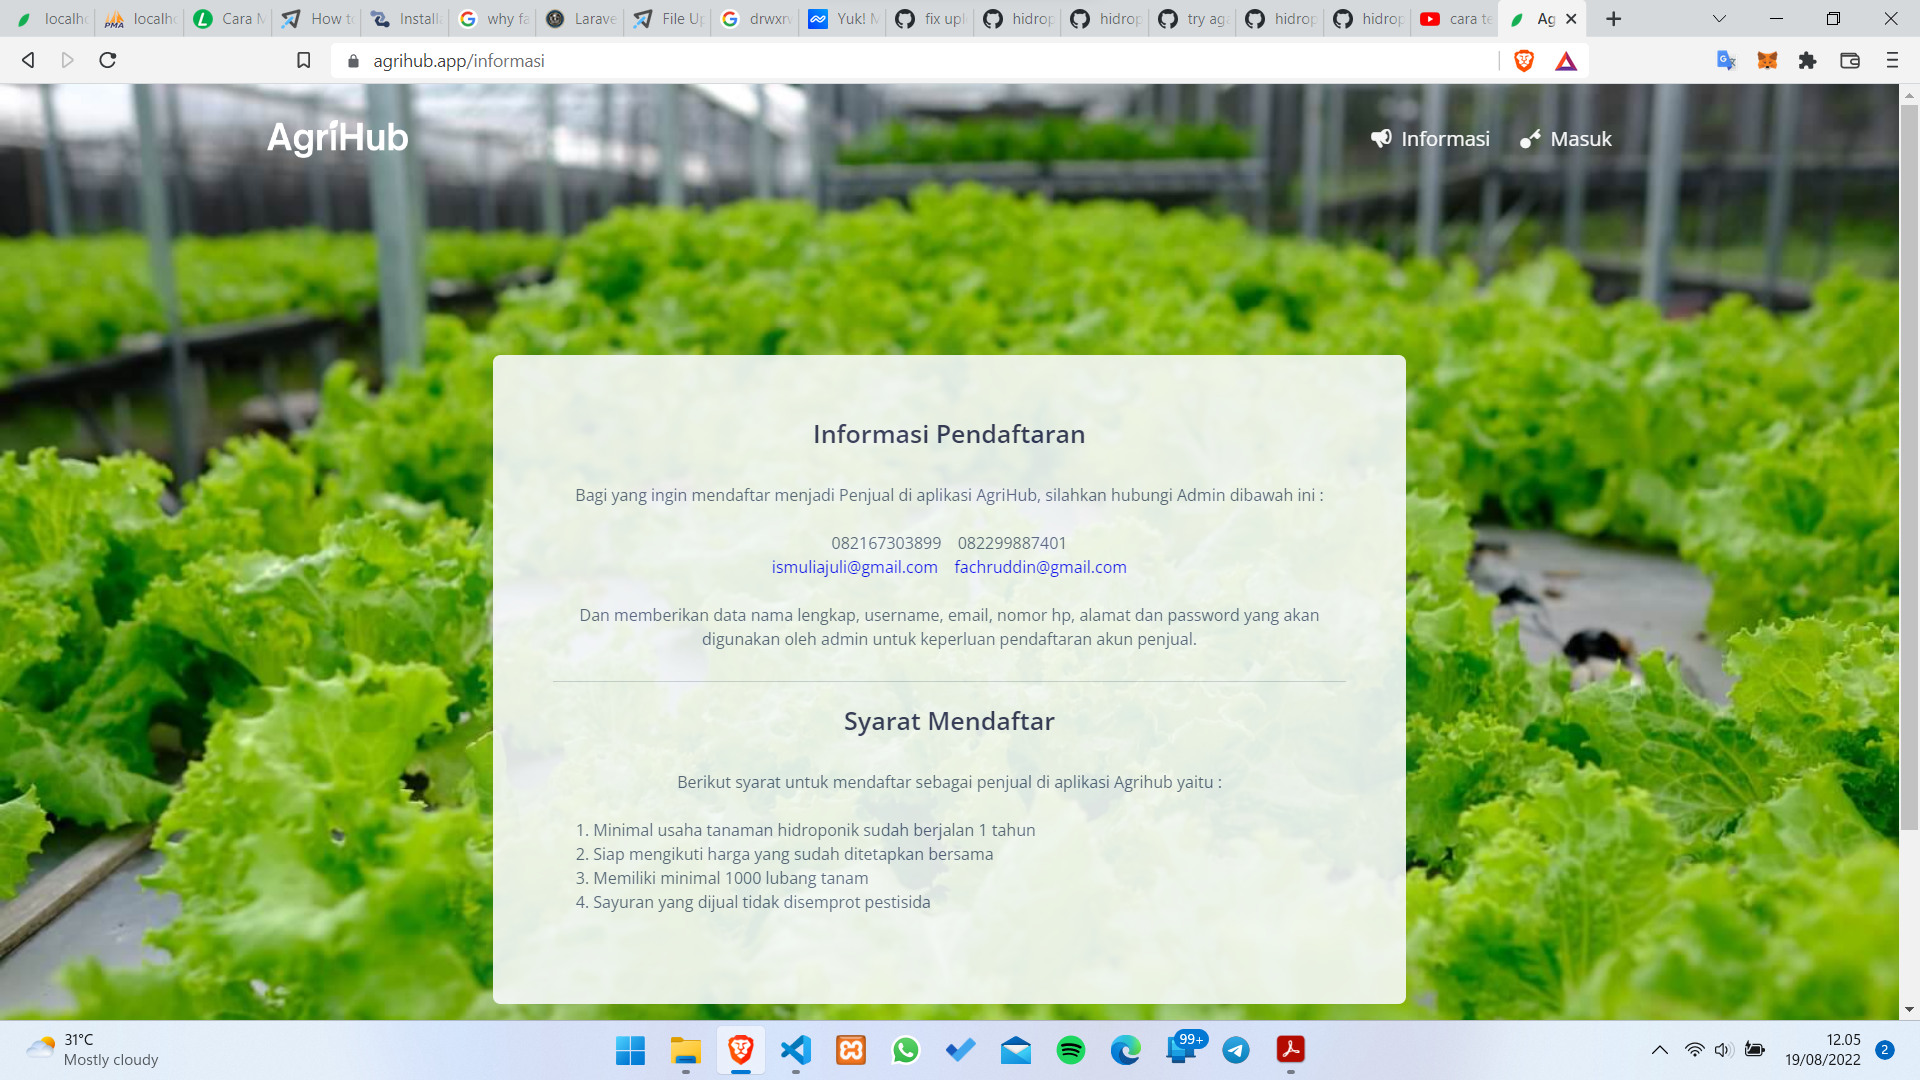
\includegraphics [width = 13.3cm, height= 8cm]{gambar/informasi}}
			\caption{Halaman Informasi}
			\label{informasi}
		\end{figure}

		\item Halaman Masuk
		\par Halaman masuk (\textit{login}) penjual sama seperti pada bagian admin, hanya saja ada sedikit perbedaan ketika akun penjual diblokir oleh admin karna melakukan kesalahan. Maka akun penjual tersebut tidak bisa masuk kedalam aplikasi. Supaya akunnya penjual dapat digunakan kembali bisa menghubungi admin terlebih dahulu. Tampilan diblokir dapat dilihat pada gambar \ref*{diblokir}.
		\begin{figure}[H]
			\centering
			{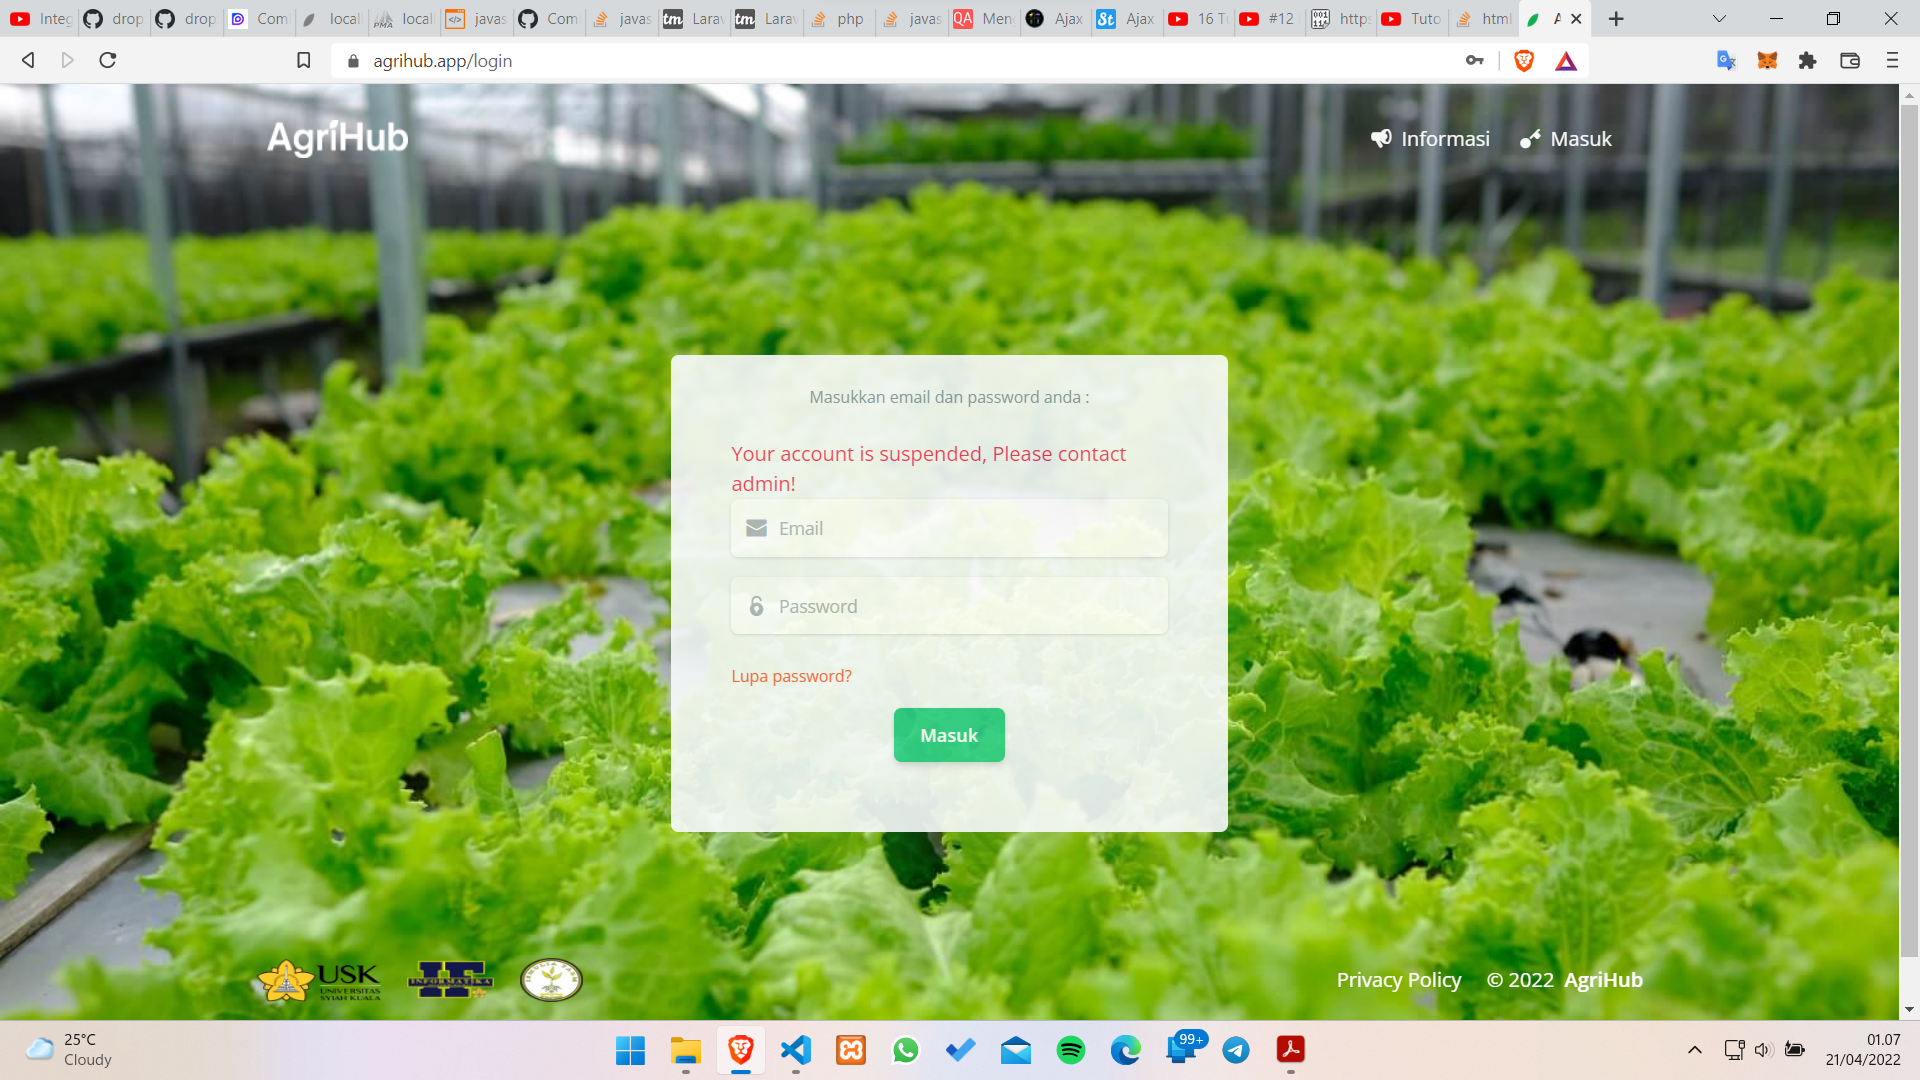
\includegraphics [width = 13.3cm, height= 8cm]{gambar/diblokir}}
			\caption{Tampilan Diblokir}
			\label{diblokir}
		\end{figure}

		\item Halaman Lupa \textit{Password}
		\par Apabila penjual lupa \textit{password} akunnya, maka dapat menklik tulisan lupa \textit{password} yang ada pada halaman masuk kemudian akan diarahkan ke halaman lupa \textit{password}. Pada halaman ini penjual dapat mengisikan emailnya, supaya nanti dikirimkan \textit{email reset password} ke alamat \textit{email} terdaftar untuk mengubah \textit{password}nya. Halaman lupa \textit{password} dapat dilihat pada gambar \ref*{lupa_password}.
		\begin{figure}[H]
			\centering
			{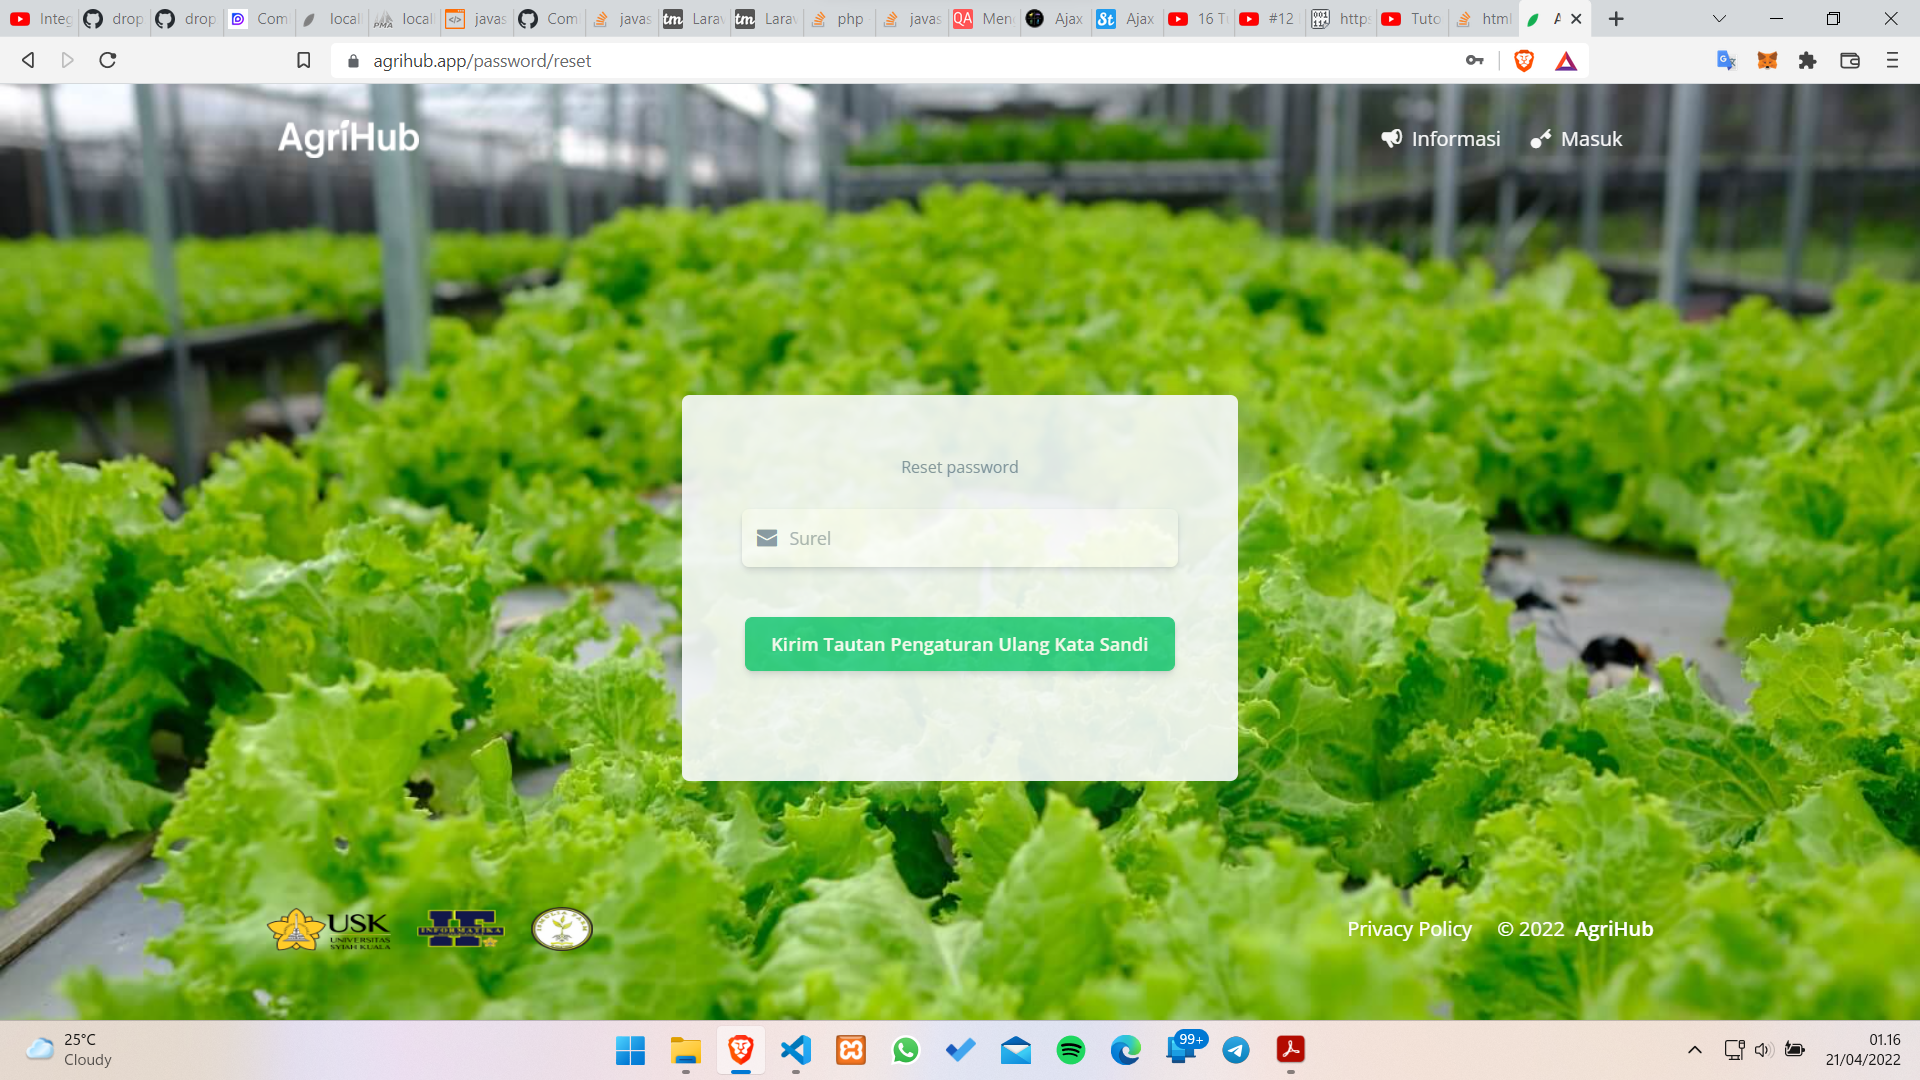
\includegraphics [width = 13.3cm, height= 8cm]{gambar/lupa_password}}
			\caption{Halaman Lupa \textit{Password}}
			\label{lupa_password}
		\end{figure}

		\newpage
		\item Halaman Dasbor
		\par Apabila penjual telah berhasil masuk kedalam aplikasi, maka akan tampil halaman dasbor yang berisi keterangan mengenai jumlah order baru yang masuk, lagi diproses, dikirim, yang sudah selesai dan jumlah order yang batal, serta jumlah ulasan yang sudah diberikan oleh pembeli. Juga ada grafik jumlah pendapatan perbulan yang sudah diperoleh oleh penjual beserta dengan jumlah pesanan yang selesai dan batal perbulannya selama 6 bulan terakhir. Halaman dasbor penjual dapat dilihat pada gambar \ref*{dashboard_penjual}.
		\begin{figure}[H]
			\centering
			{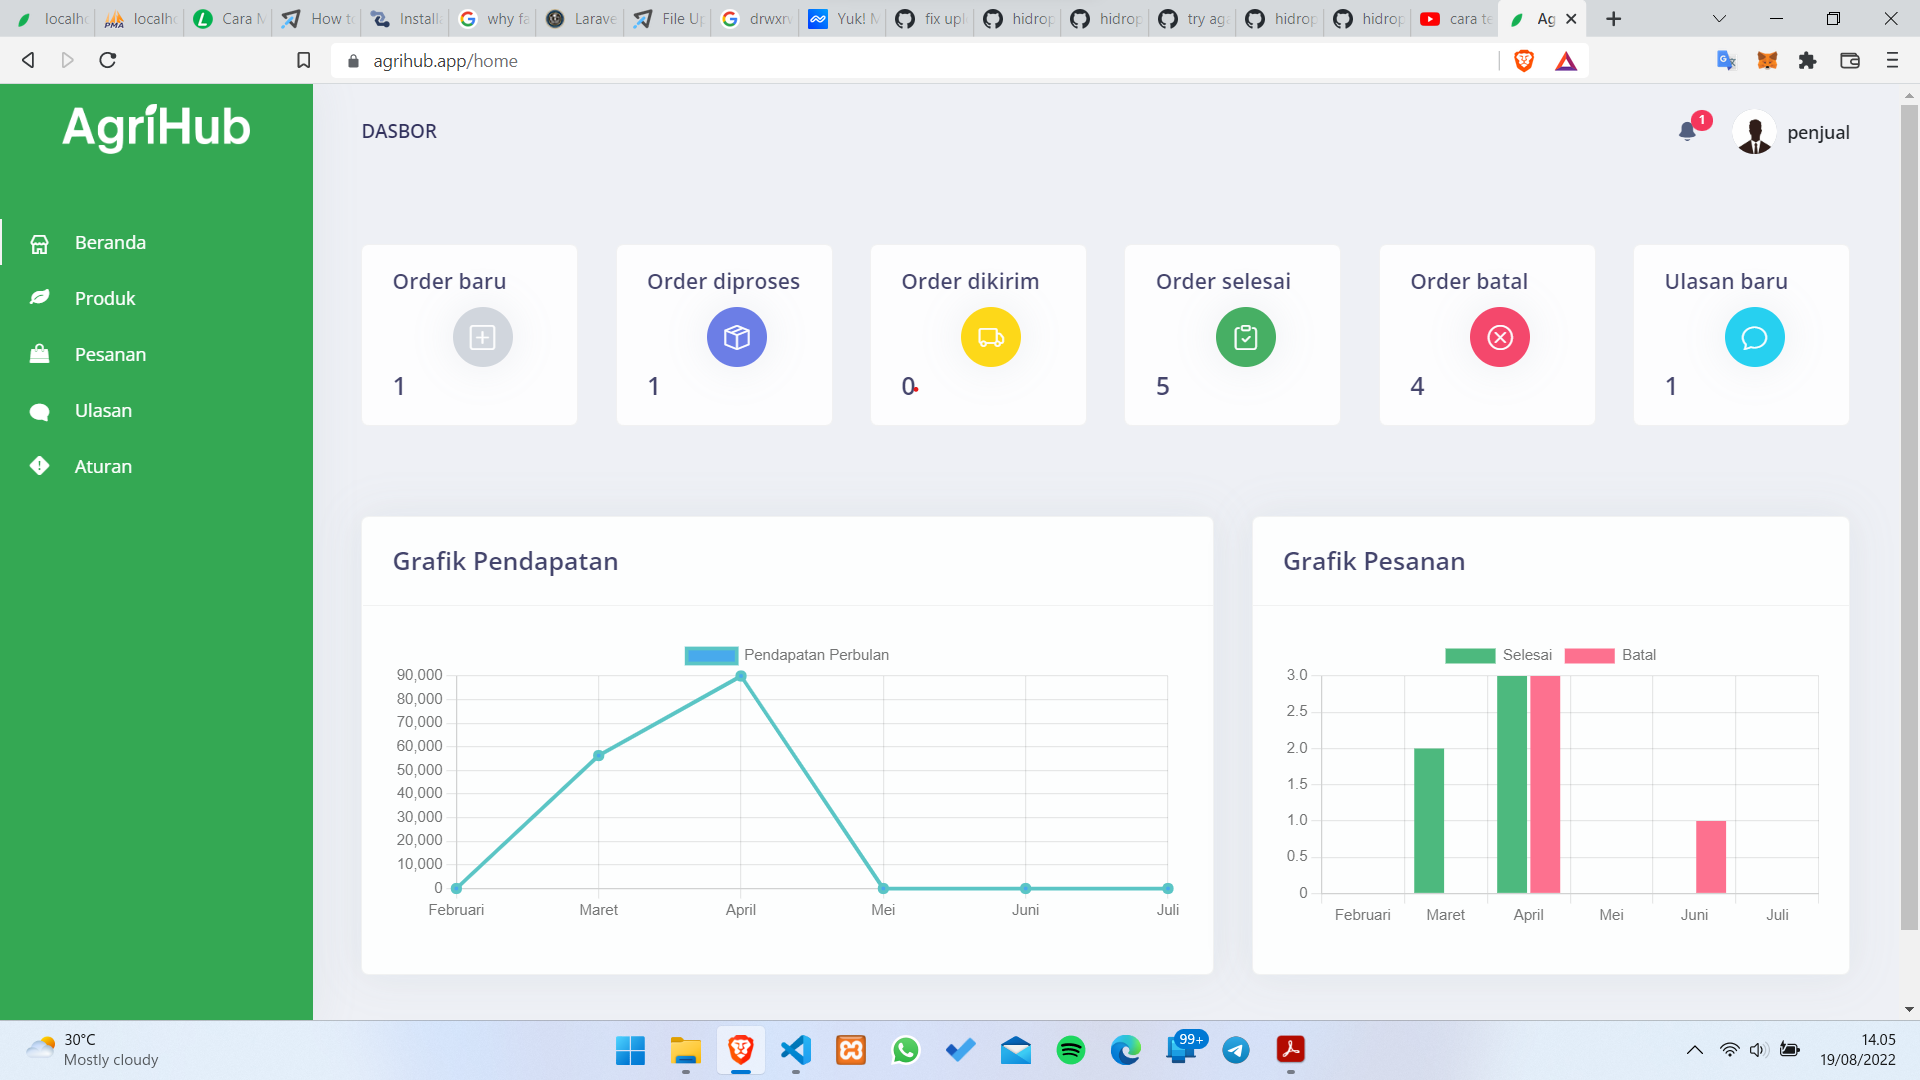
\includegraphics [width = 13.3cm, height= 8cm]{gambar/penjual/dashboard_penjual}}
			\caption{Halaman Dasbor pada sisi Penjual}
			\label{dashboard_penjual}
		\end{figure}

		\item Halaman Produk
		\par Pada halaman produk ini penjual dapat mengelola produknya yang ingin dijual seperti menambahkan produk baru, mengubah data produk yang sudah ada atau menghapus produk yang tidak ingin dijual lagi. Apabila penjual ingin menambahkan produk baru dapat melakukannya dengan menekan tombol tambah, maka akan muncul tampilan tambah produk dan mengisi data-data produk seperti gambar, nama, harga, stok, satuan, jumlah per satuan dan keterangan. Ada juga kolom promo yang bersifat opsional yang bisa dipakai oleh penjual jika admin menyediakan promo. Jika penjual ingin mengubah data produk dapat menekan tombol ubah yang akan diarahkan ke halaman ubah produk dan jika ingin menghapus produk dapat menekan tombol hapus. Halaman produk dan tampilan tambah produk dapat dilihat pada gambar berikut ini.
		\begin{figure}[H]
			\centering
			{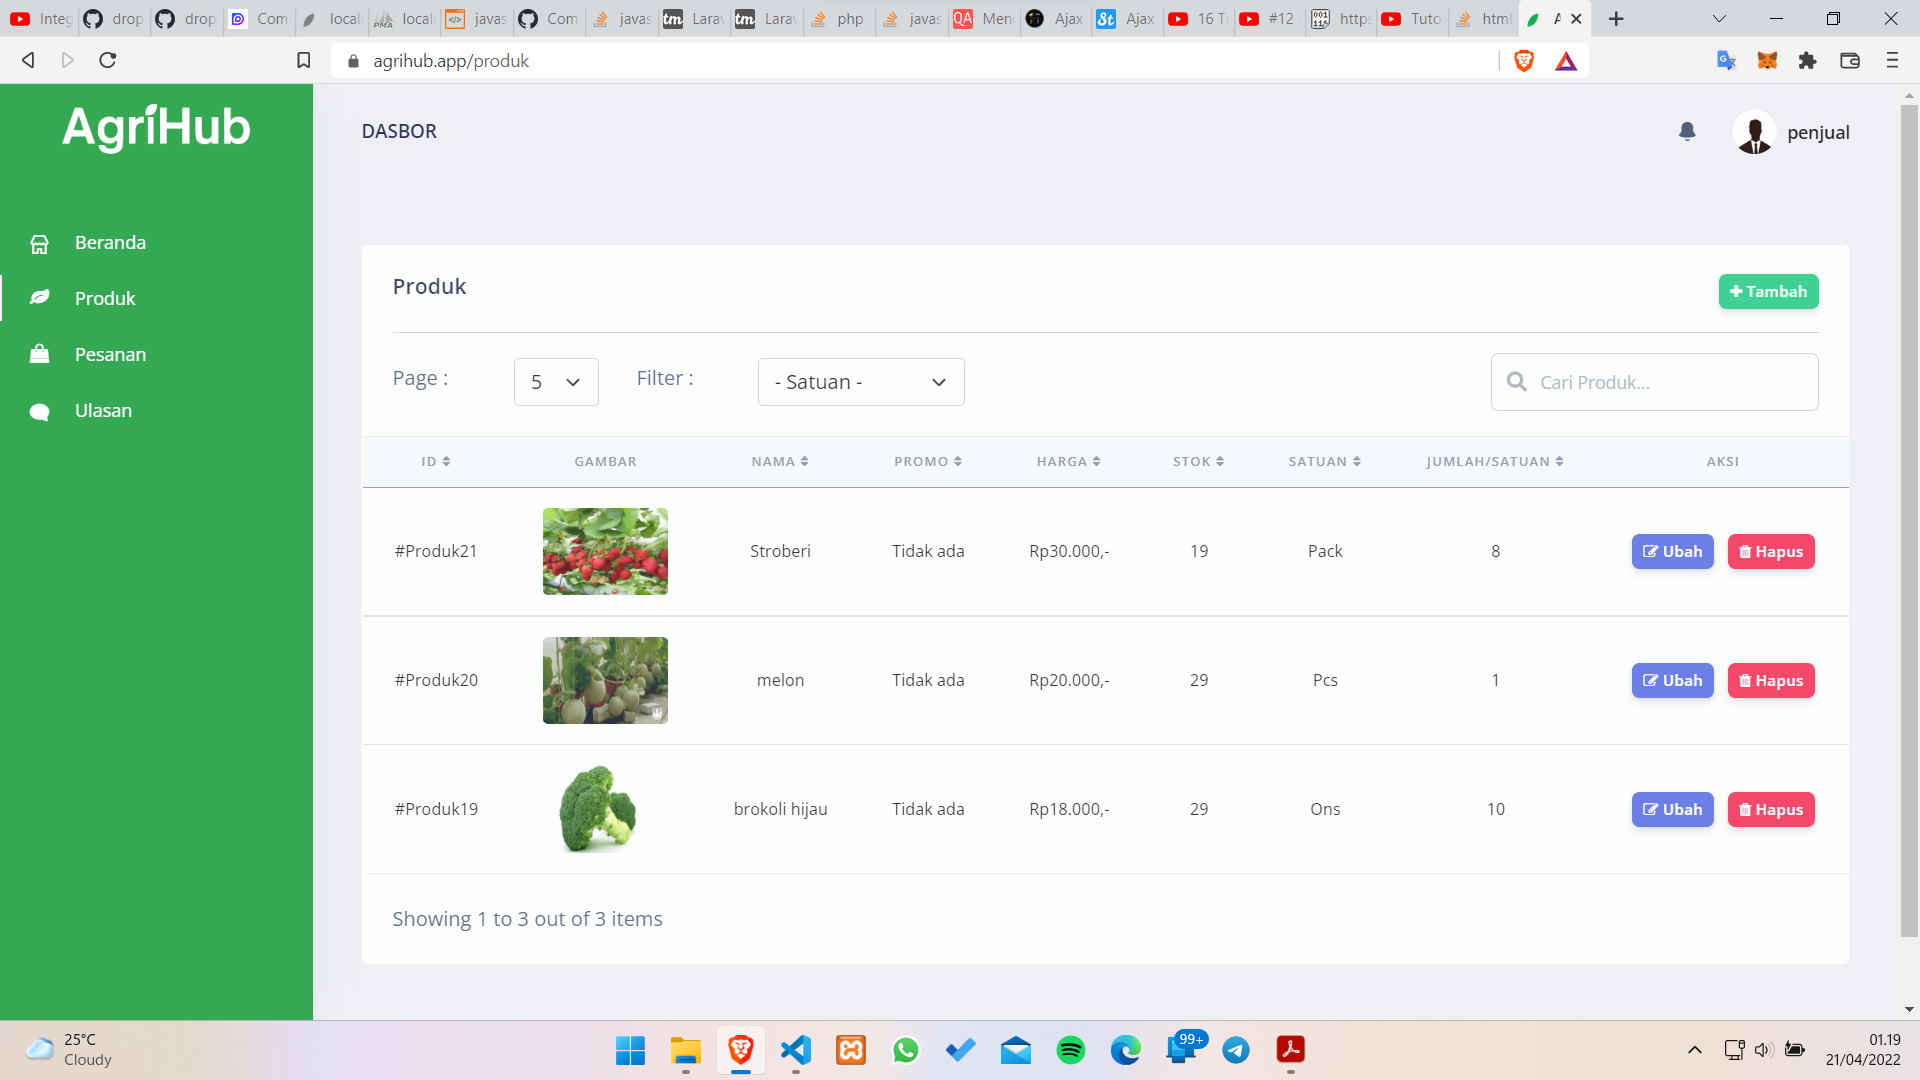
\includegraphics [width = 13.3cm, height= 8cm]{gambar/penjual/produk_penjual}}
			\caption{Halaman Produk pada sisi Penjual}
			\label{produk_penjual}
		\end{figure}
		\begin{figure}[H]
			\centering
			{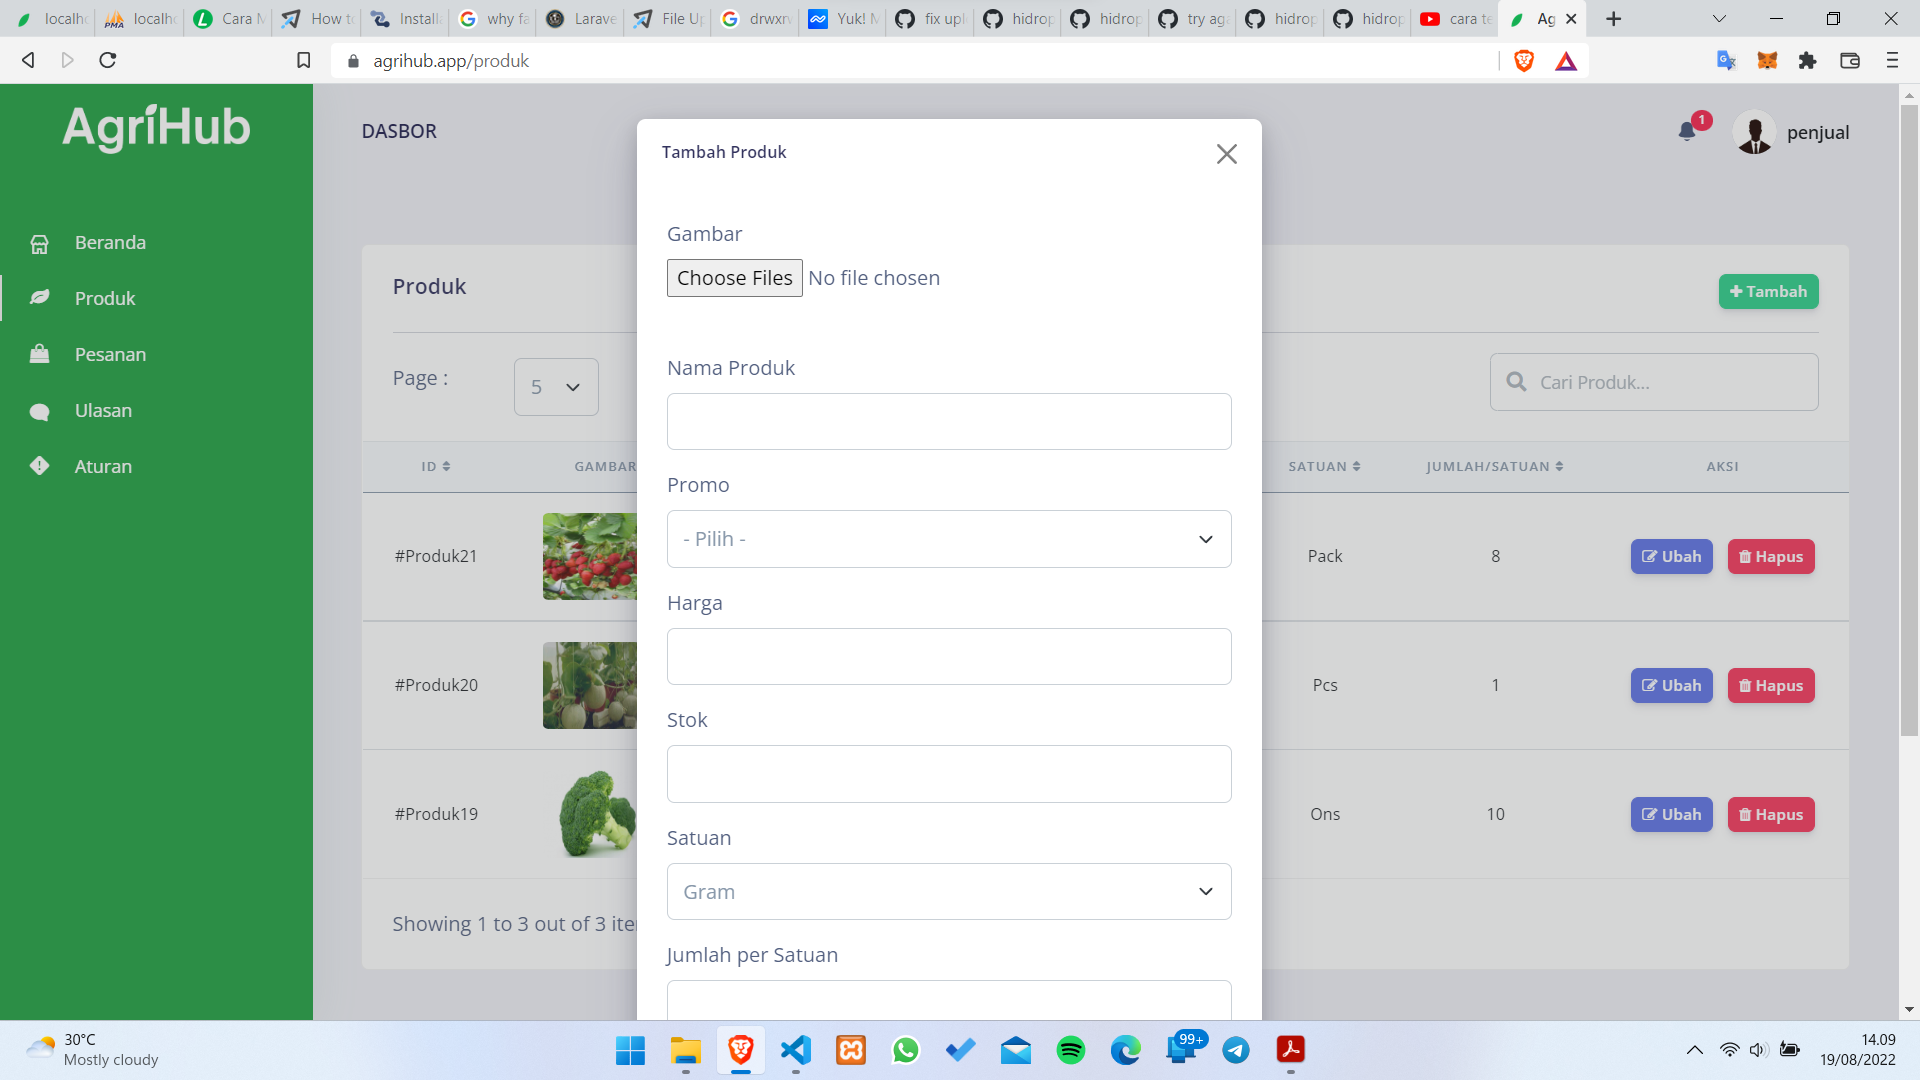
\includegraphics [width = 13.3cm, height= 8cm]{gambar/penjual/tambah_produk}}
			\caption{Tampilan Tambah Produk}
			\label{tambah_produk}
		\end{figure}

		\item Halaman Ubah Produk
		\par Penjual dapat mengubah detail produk yang ia jual melalui halaman ubah produk ini. Disini penjual dapat menambah atau menghapus gambar produk dan dapat mengubah detail produknya seperti nama, harga, stok, satuan dan lainnya. Halaman ubah produk dapat dilihat pada gambar \ref*{ubah_produk}.
		\begin{figure}[H]
			\centering
			{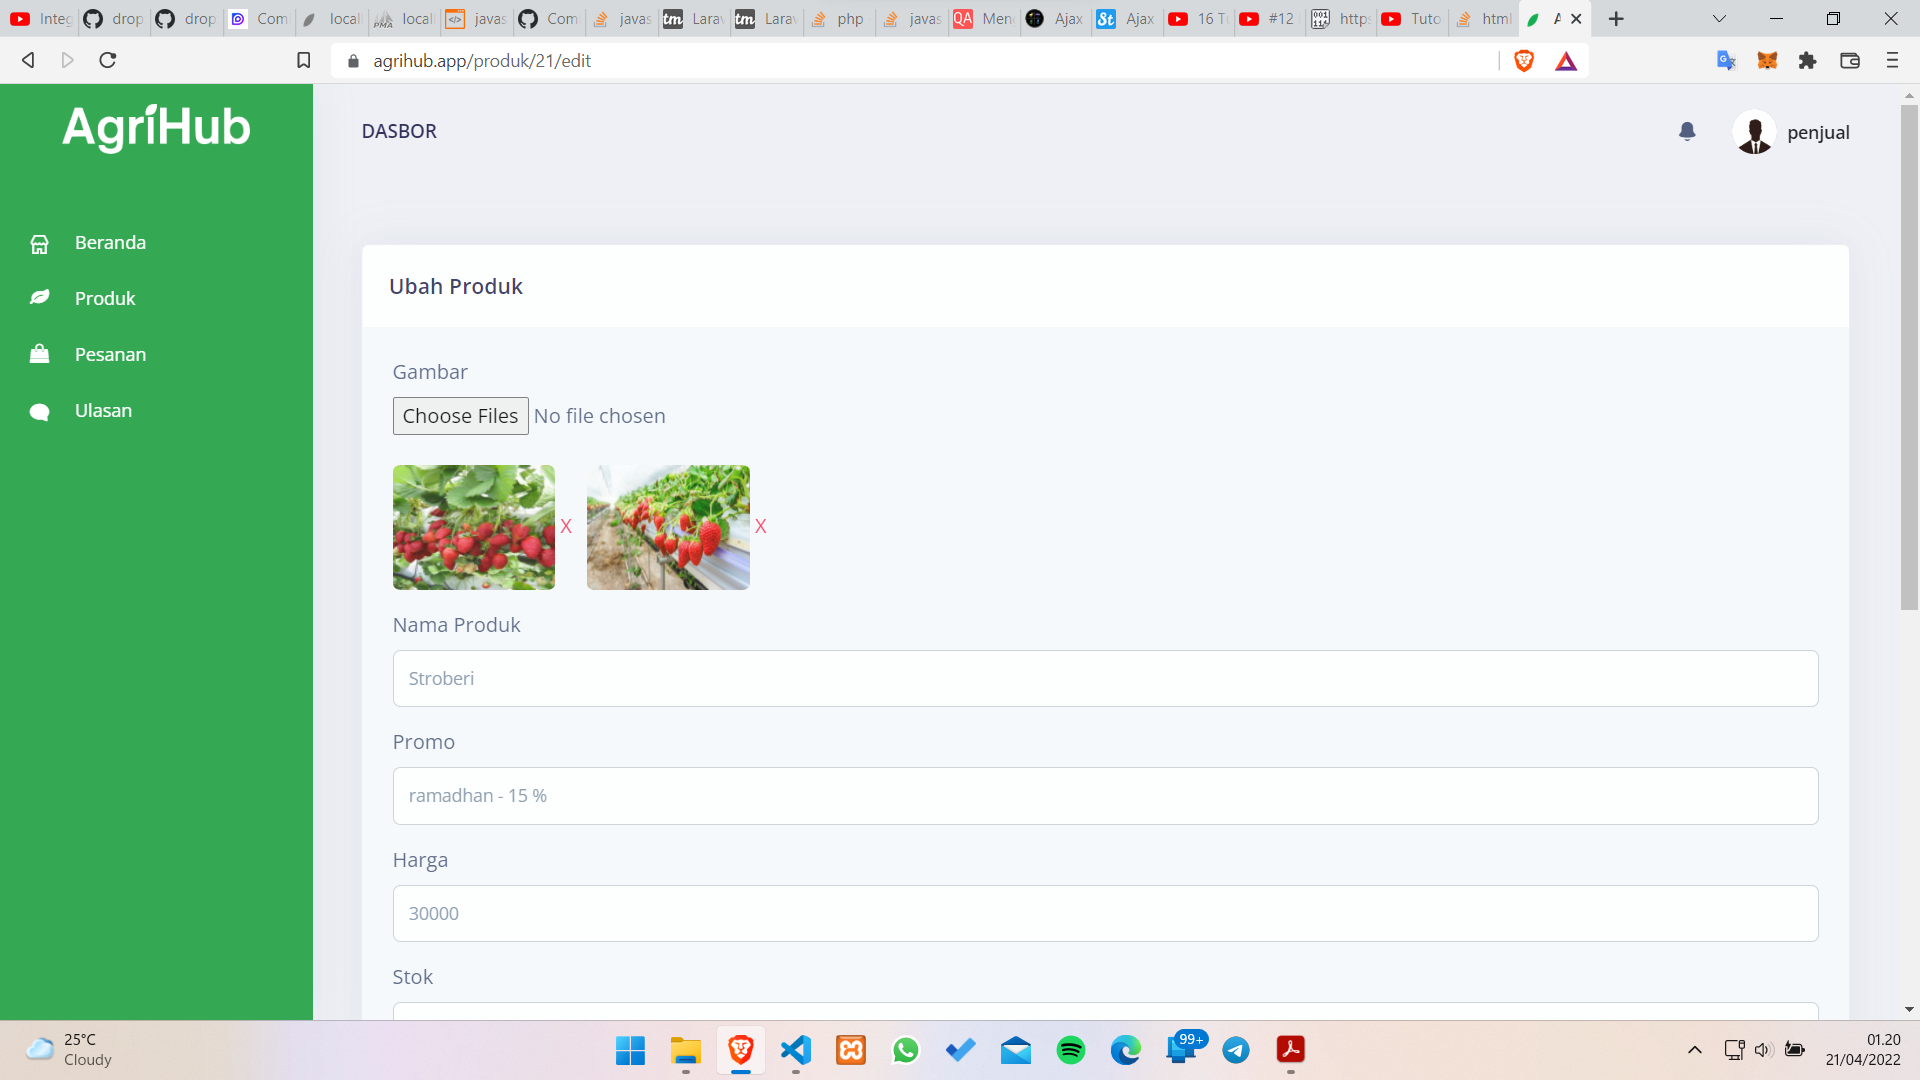
\includegraphics [width = 13.3cm, height= 8cm]{gambar/penjual/ubah_produk}}
			\caption{Halaman Ubah Produk}
			\label{ubah_produk}
		\end{figure}

		\item Halaman Pesanan
		\par Selanjutnya ada halaman pesanan, halaman ini merupakan halaman yang paling penting bagi penjual karna pada halaman ini penjual mengelola semua pesanan yang masuk dari pembeli. Penjual dapat mengetahui informasi mengenai pesanannya seperti tanggal, jam, nama pembeli, jumlah item, ongkos kirim dan total harganya beserta status pesanannya. Halaman pesanan pada sisi penjual dapat dilihat pada gambar \ref*{pesanan_penjual} dibawah ini.
		\begin{figure}[H]
			\centering
			{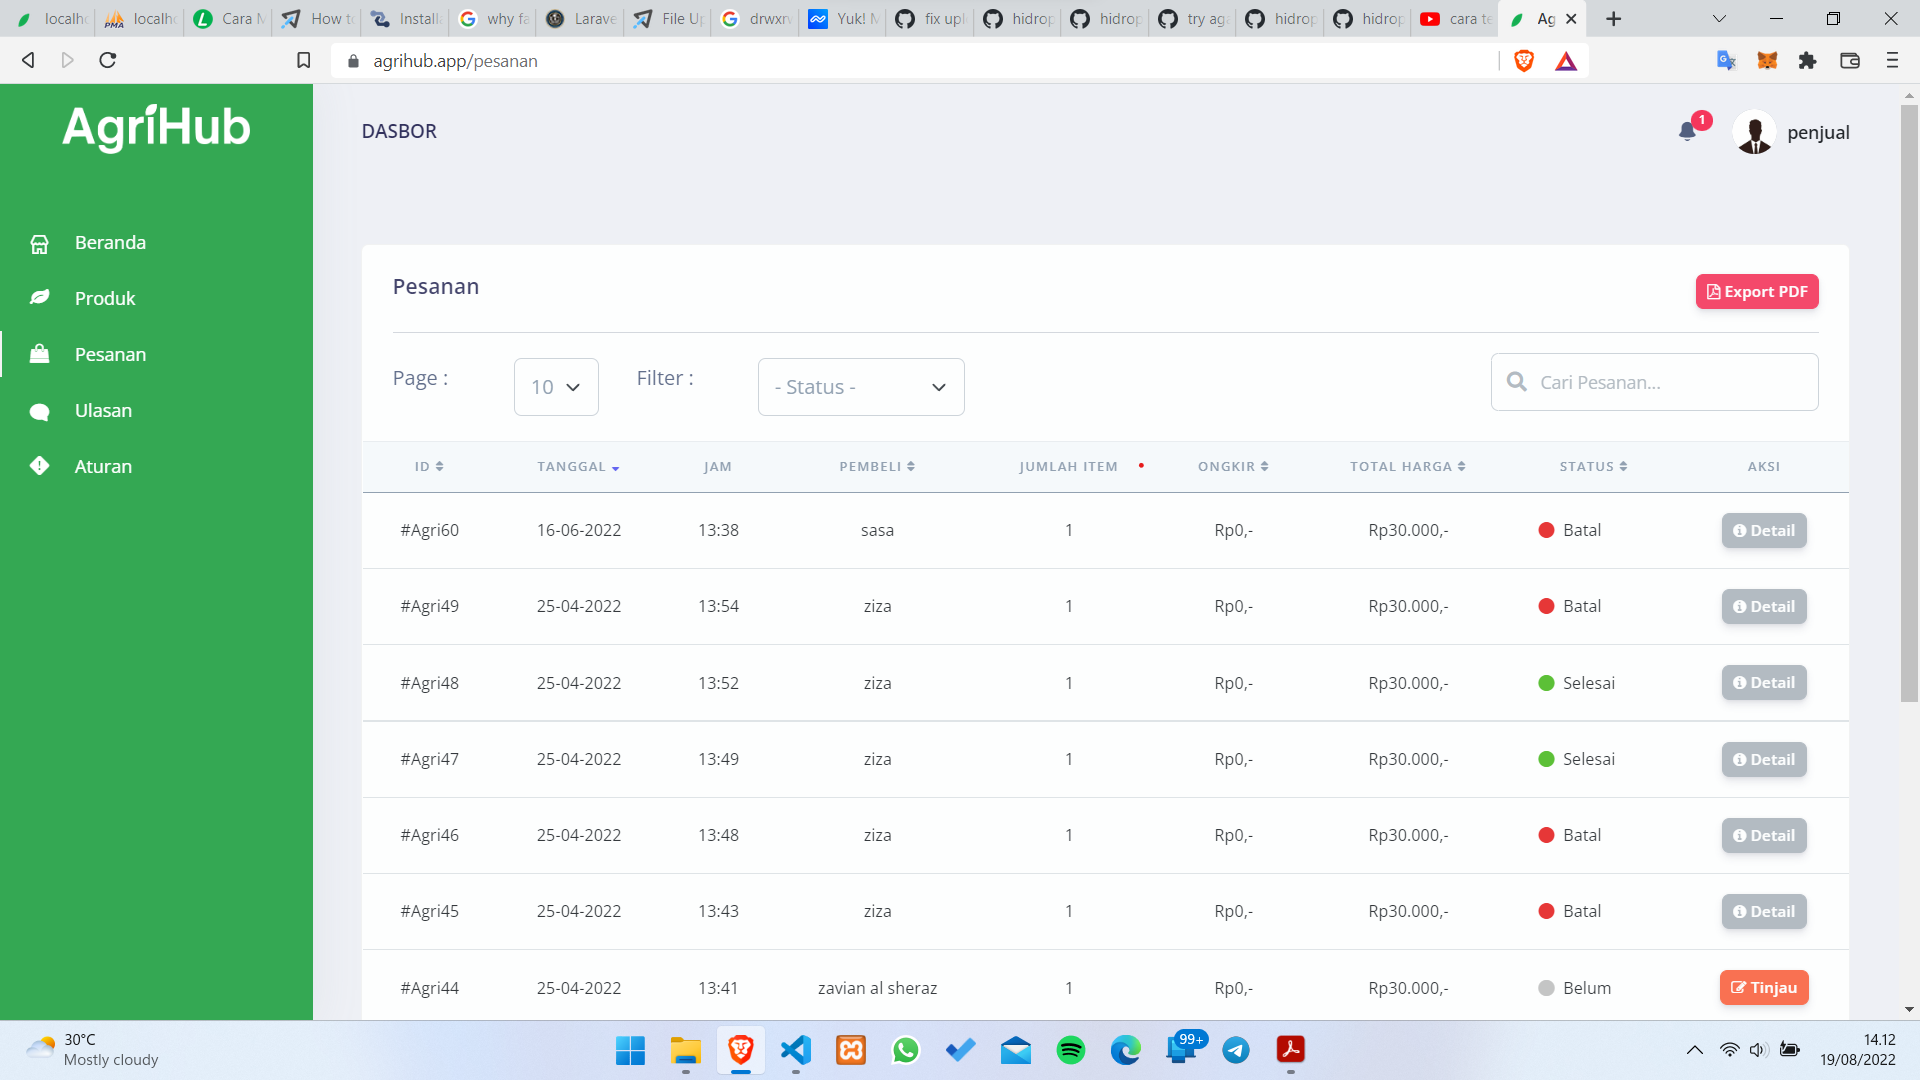
\includegraphics [width = 13.3cm, height= 8cm]{gambar/penjual/pesanan_penjual}}
			\caption{Halaman Pesanan pada sisi Penjual}
			\label{pesanan_penjual}
		\end{figure}
		\newpage
		\par Jika penjual ingin memproses pesanan dari pembeli maka dapat menekan tombol tinjau yang berwarna \textit{orange}, lalu mengisi harga ongkos kirimnya dan mengubah status pesanannya dari belum menjadi diproses. Tombol ini hanya tampil ketika status pesanannya masih belum diproses, lagi diproses dan dikirim. Namun apabila sudah selesai atau batal maka akan tampil tombol detail. Penjual dapat menghubungi pembeli disini melalui tombol WhatApps apabila ada yang ingin ditanyakan lebih lanjut kepada pembeli. Dan penjual juga dapat menolak pesanannya dengan mengubah status pesanan menjadi batal. Tampilan tinjau pesanan dapat dilihat pada gambar \ref*{tinjau_pesanan}.
		\begin{figure}[H]
			\centering
			{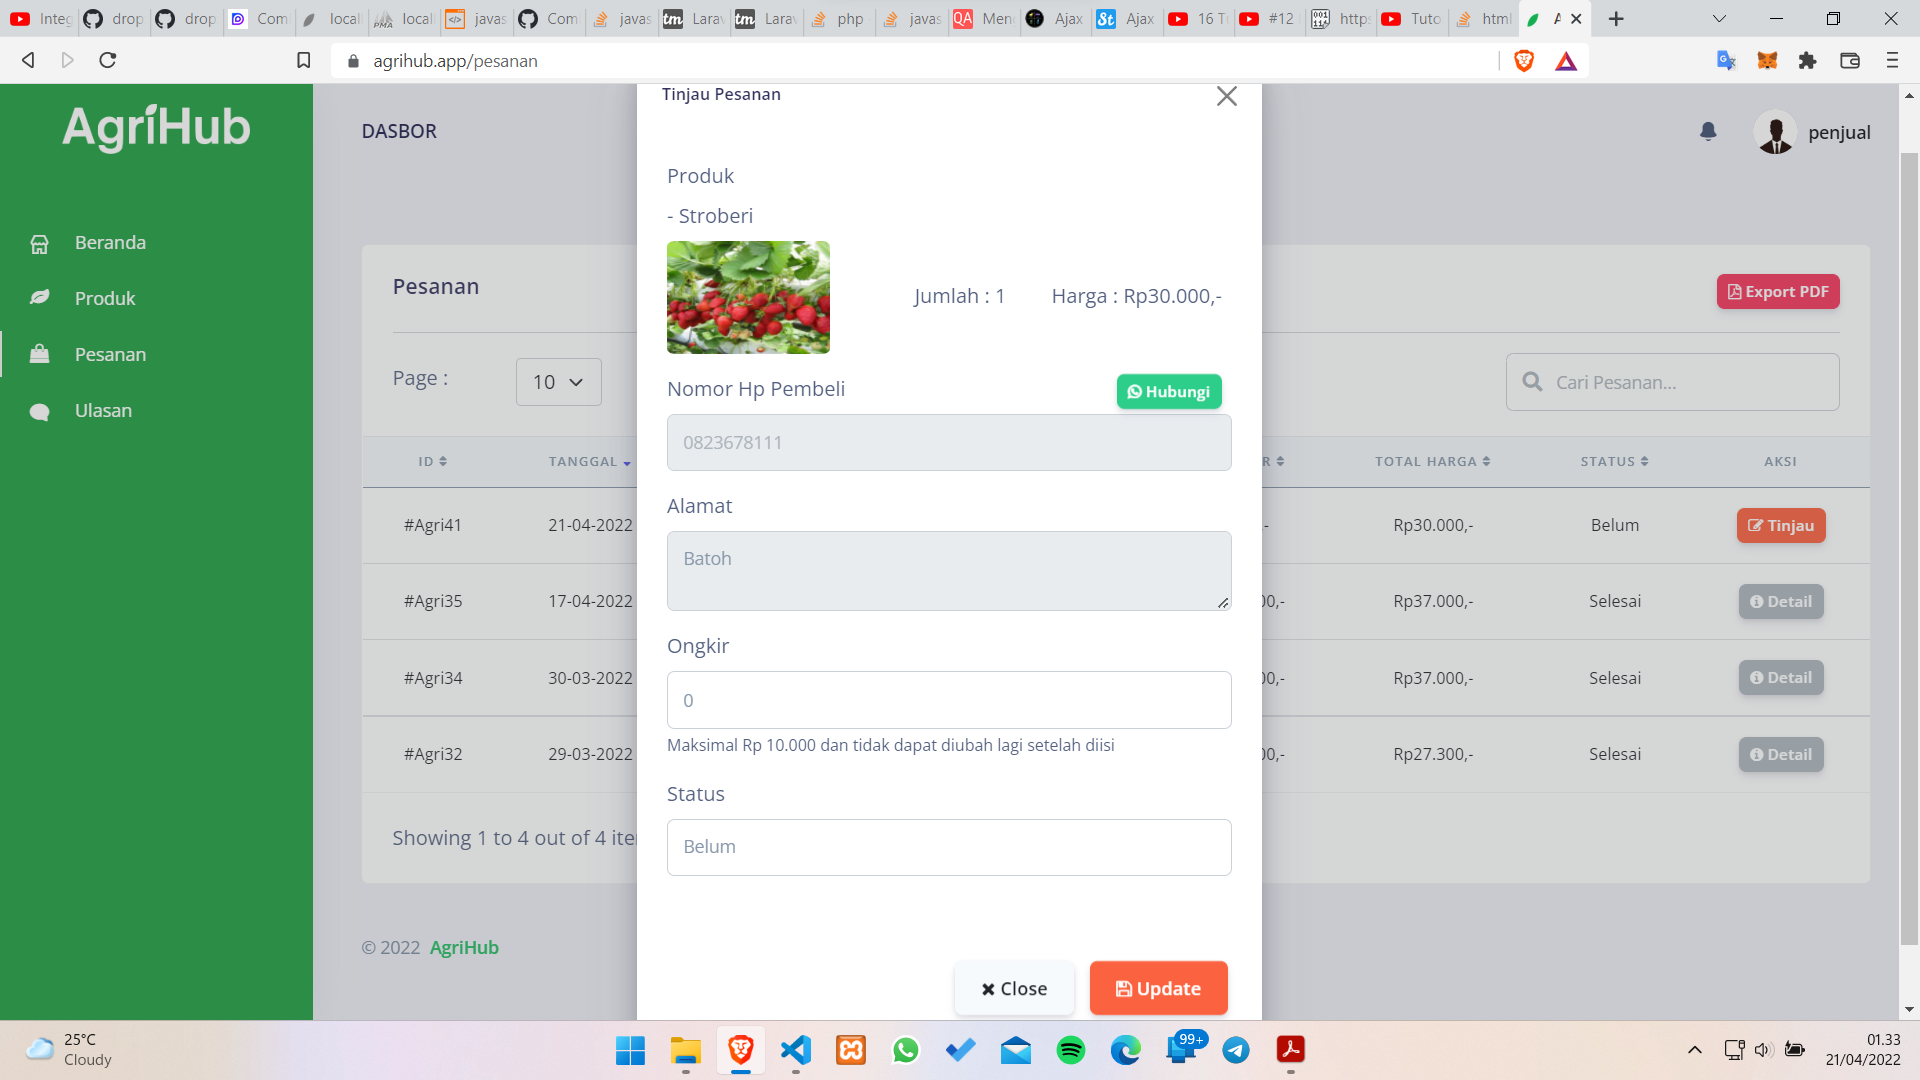
\includegraphics [width = 13.3cm, height= 8cm]{gambar/penjual/tinjau_pesanan}}
			\caption{Tampilan Tinjau Pesanan}
			\label{tinjau_pesanan}
		\end{figure}
		\par Apabila penjual ingin melihat daftar pesananya dalam bentuk pdf dapat melakukannya dengan menekan tombol \textit{export} pdf yang berwarna merah, maka akan muncul tampilan hasilnya dalam bentuk pdf. Tampilan ekspor pdf pesanan pada sisi penjual dapat dilihat pada gambar \ref*{pdf_penjual}.
		\begin{figure}[H]
			\centering
			{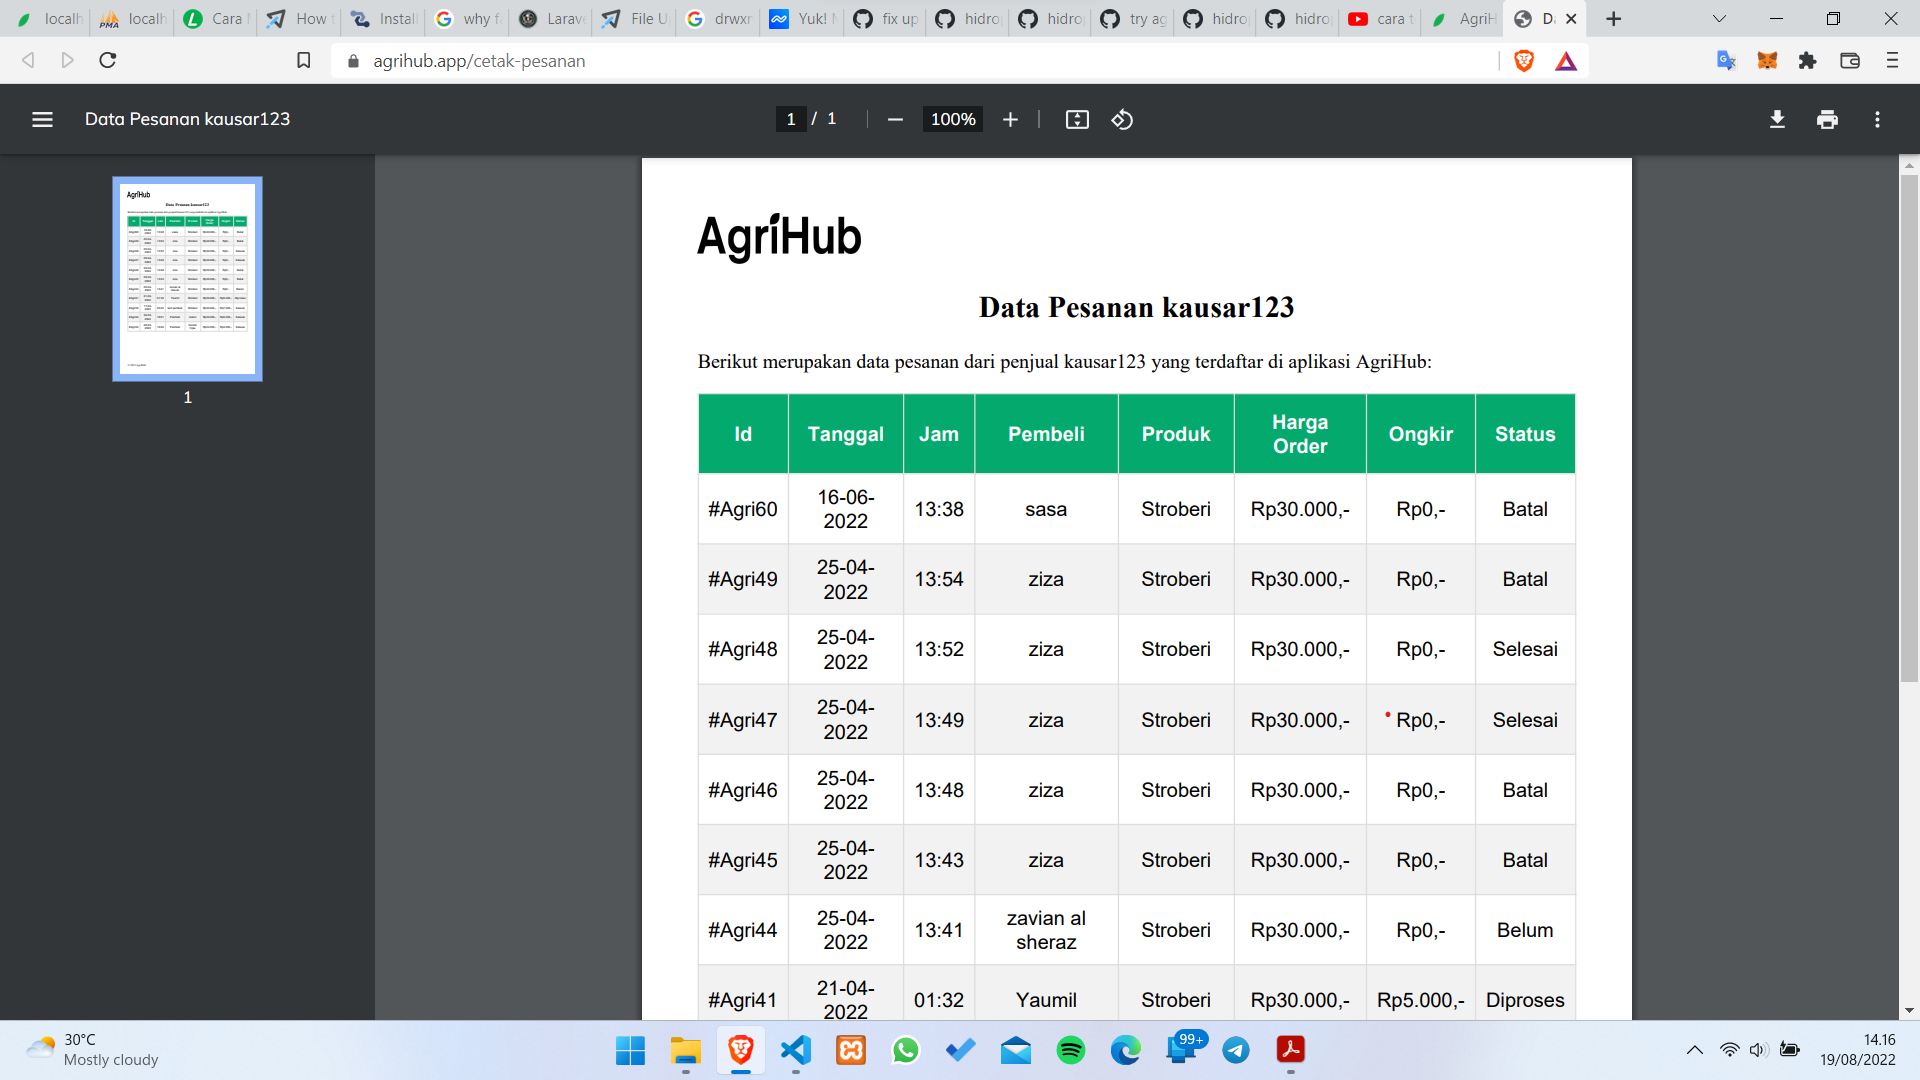
\includegraphics [width = 13.3cm, height= 8cm]{gambar/penjual/pdf_penjual}}
			\caption{Tampilan Ekspor PDF Pesanan pada sisi Penjual}
			\label{pdf_penjual}
		\end{figure}

		\item Halaman Ulasan
		\par Pada halaman ulasan ini penjual dapat melihat semua ulasan yang sudah diberikan oleh pembelinya terhadap produk yang ia jual. Dari ulasan ini dapat menjadi masukan bagi penjual untuk meningkatkan lagi kualitas produk yang ia tawarkan. Penjual juga dapat menfilter ulasannya berdasarkan ratingnya dan dapat menghapus ulasan dari pembeli jika dinilai ulasannya mengandung kata-kata yang tidak pantas. Halaman ulasan pada sisi penjual dapat dilihat pada gambar \ref*{ulasan}.
		\begin{figure}[H]
			\centering
			{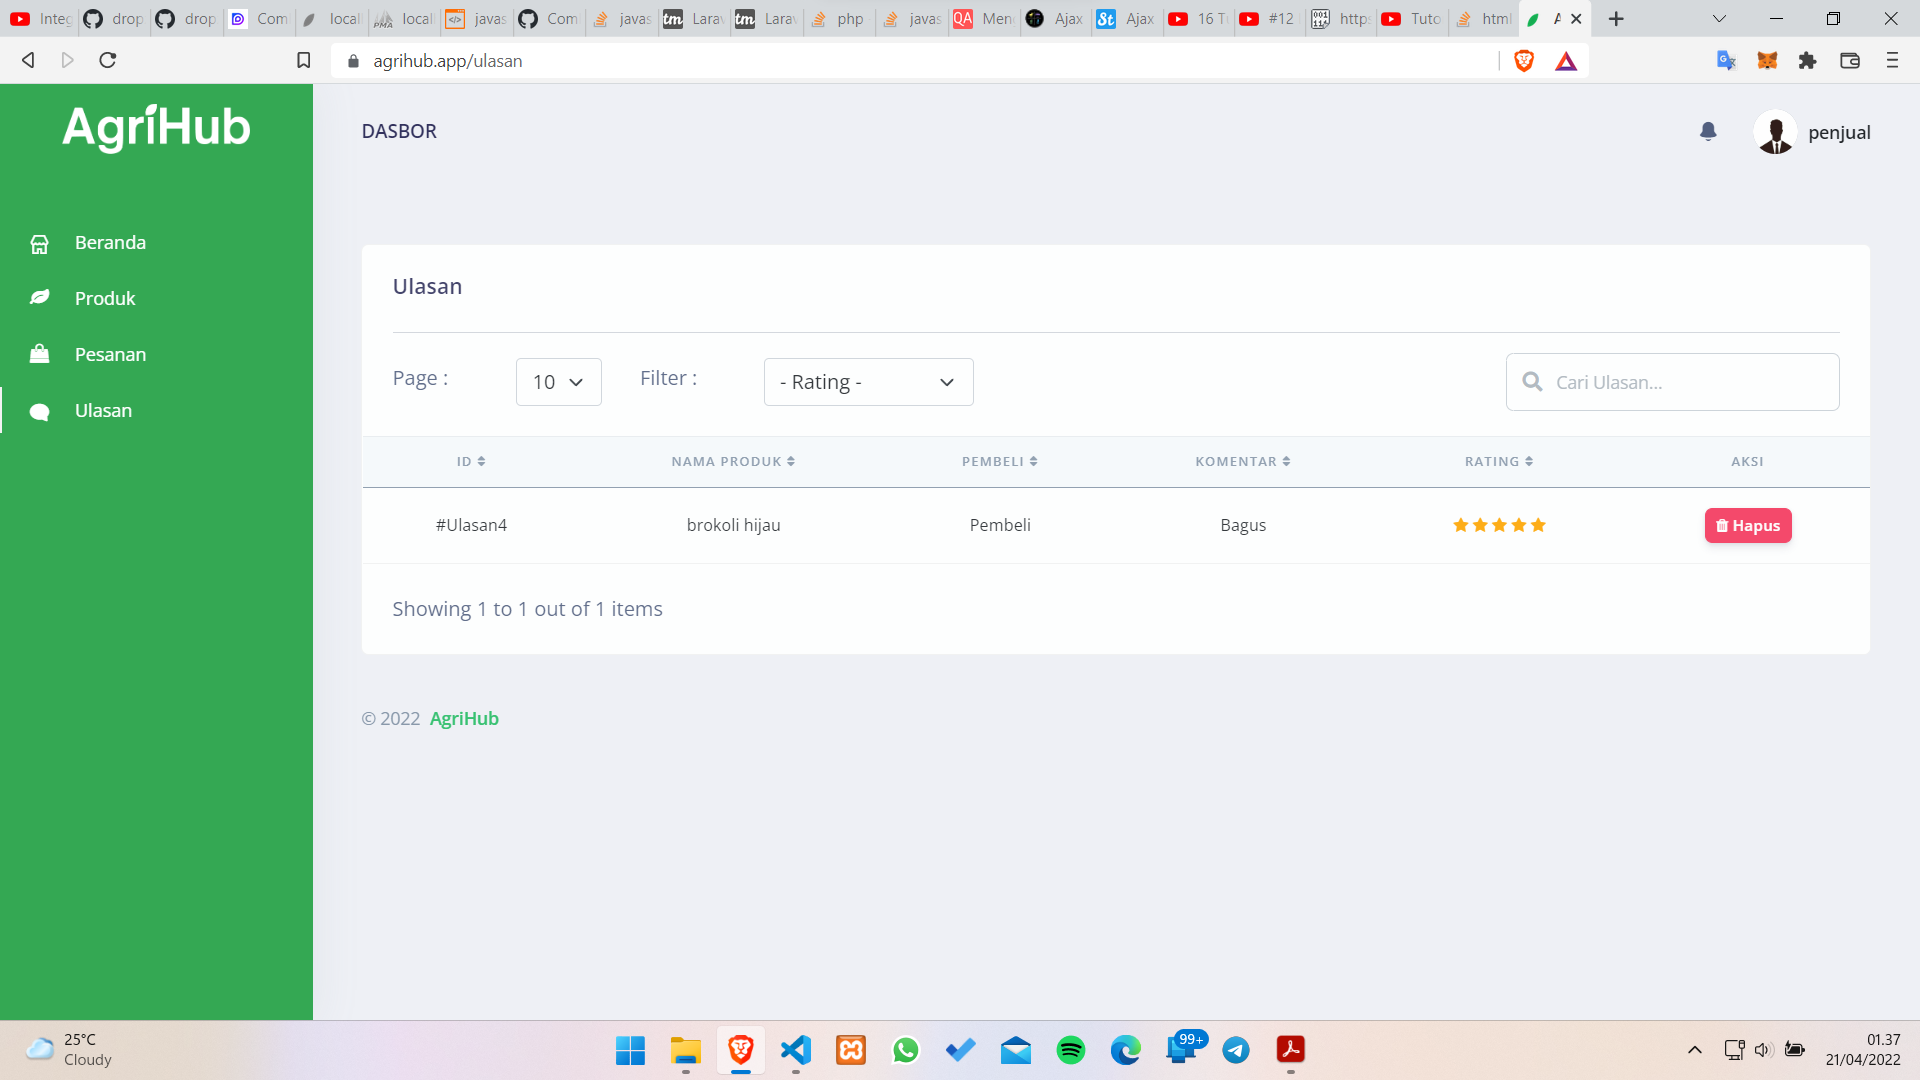
\includegraphics [width = 13.3cm, height= 8cm]{gambar/penjual/ulasan}}
			\caption{Halaman Ulasan pada sisi Penjual}
			\label{ulasan}
		\end{figure}

		\item Halaman Ubah Profil
		\par Terakhir ada halaman profil yaitu halaman dimana penjual dapat mengubah informasi mengenai akunnya seperti foto, nama, nomor hp dan alamat serta \textit{password}. Halaman ubah profil dapat dilihat pada gambar \ref*{profil}.
		\begin{figure}[H]
			\centering
			{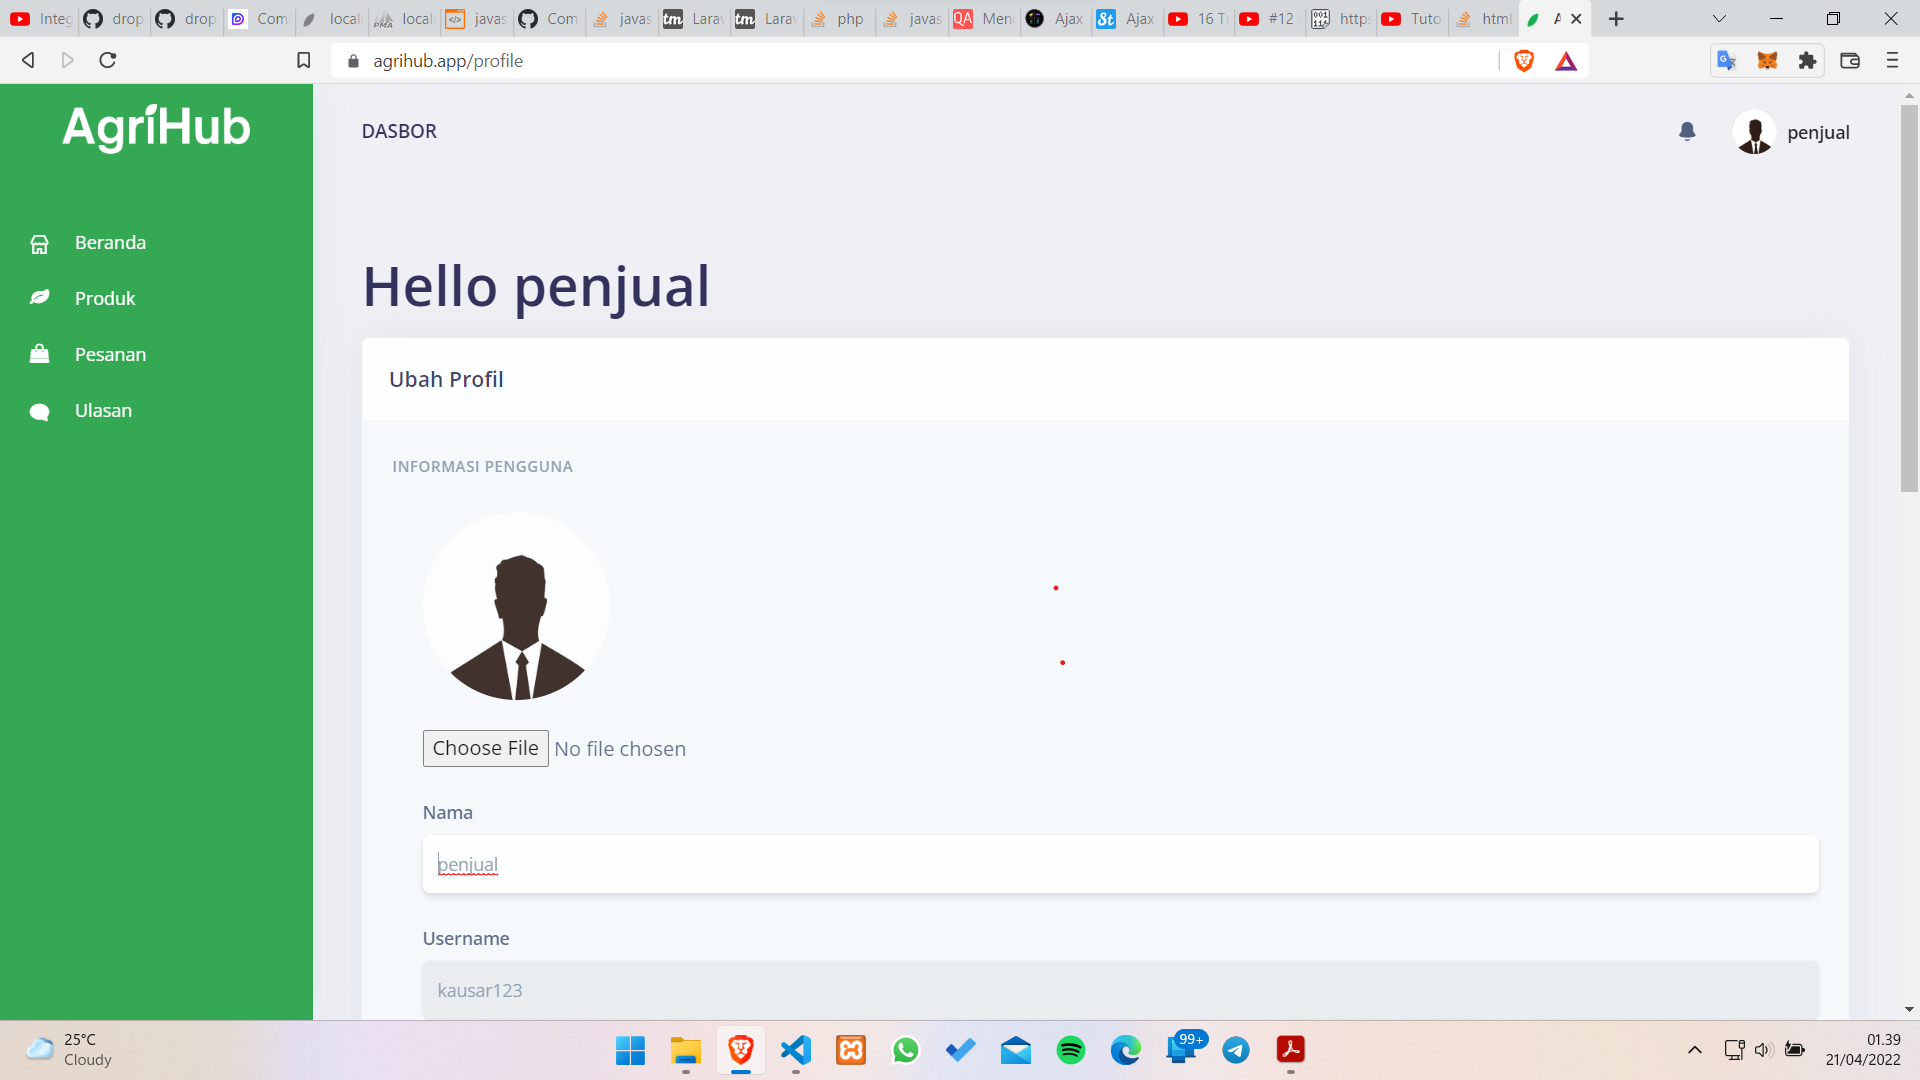
\includegraphics [width = 13.3cm, height= 8cm]{gambar/penjual/profil}}
			\caption{Halaman Ubah Profil}
			\label{profil}
		\end{figure}
	\end{enumerate}
\end{enumerate}

\section{\uppercase{Implementasi Sistem}}
Aplikasi penjualan tanaman hidroponik berbasis web dibangun
menggunakan \textit{framework} Laravel sebagai alat (\textit{tool}) untuk membangun aplikasi dan \textit{database} MySQL sebagai penyimpanan datanya. Pada aplikasi ini juga dibuatkan API untuk menghubungkan aplikasi android dengan aplikasi web yang bertindak sebagai \textit{web service} untuk digunakan pada aplikasi berbasis android. Aplikasi penjualan tanaman hidroponik ini juga sudah memiliki sertifikat Hak Kekayaan Intelektual (HKI) dengan nomor EC00202153108 yang dapat dilihat pada lampiran 1.

% \par Adapun proses implementasi sistem menggunakan metode \textit{scrum}. Metode \textit{scrum} terdiri dari kumpulan \textit{product backlog} yang merupakan daftar tugas yang harus dikerjakan dengan prioritasnya masing-masing. Kemudian kumpulan \textit{product backlog} tersebut diimplementasikan dalam bentuk kode pemrograman yang dibagi dalam beberapa kali iterasi atau disebut \textit{sprint}. Pada penelitian ini, terdapat 4 kali iterasi \textit{sprint}. Berikut merupakan pembagian \textit{product backlog} ke dalam beberapa iterasi :

\par Adapun proses implementasi sistem menggunakan metode \textit{scrum}. Metode \textit{scrum} terdiri dari \textit{product backlog} yang berisi daftar fitur yang akan diterapkan ke dalam aplikasi. \textit{Product backlog} dibuat berdasarkan \textit{user story} yang telah diperoleh pada hasil analisis kebutuhan pengguna. Kemudian \textit{product backlog} tersebut diimplementasikan dalam bentuk kode program yang dibagi dalam beberapa kali iterasi atau disebut \textit{sprint}. Pada penelitian ini, terdapat 4 kali iterasi. Berikut merupakan pembagian \textit{product backlog} ke dalam beberapa iterasi :

% Metode \textit{scrum} terdiri dari kumpulan \textit{product backlog} yang merupakan daftar pekerjaan yang harus dikerjakan dengan prioritasnya masing-masing.

% Metode \textit{scrum} terdiri dari \textit{product backlog} yang berisi daftar dari fitur yang akan diterapkan ke dalam sistem.

% \textit{Product backlog} dibuat berdasarkan \textit{user story} yang telah diperoleh pada hasil analisis kebutuhan pengguna.

\newpage
\begin{enumerate}
	\item \textit{Sprint} Pertama
	\par Pada \textit{sprint} pertama ini, merupakan tahap awal pembuatan aplikasi seperti membuat \textit{file migration} untuk \textit{database}, \textit{Models} untuk setiap tabel dan relasinya, fungsi \textit{login}, fitur \textit{upload} produk dan beberapa tampilan (\textit{view}) halaman aplikasi serta API dasar untuk digunakan pada aplikasi android. Adapun daftar \textit{product backlog} pada \textit{sprint} yang pertama dapat dilihat pada tabel \ref*{tab:sprint pertama} berikut ini.

	% fitur yang difokuskan pada \textit{sprint} ini merupakan fitur-fitur dengan prioritas tinggi seperti membuat file migration untuk database, buat fungsi login dan beberapa view halaman serta API dasar untuk digunakan pada aplikasi android. Adapun untuk daftar \textit{product backlog} pada \textit{sprint} yang pertama dapat dilihat pada tabel \ref*{tab:sprint pertama} berikut ini.

	\addtocounter{table}{+1}
	\begin{table}[H]
		\begin{center}
		\caption{\textit{Product Backlog sprint} pertama}
		\label{tab:sprint pertama}
		% \footnotesize
		\begin{tabular}{|l|c|}
		\hline
		\multicolumn{1}{|c|}{Item} & Prioritas\\
		\hline
		Buat \textit{file migration} untuk \textit{database} & Tinggi\\
		\hline
		Buat \textit{Models} untuk setiap tabel dan relasinya & Tinggi\\
		\hline
		Implementasi \textit{template bootstrap} Argon & Rendah\\
		\hline
		Buat \textit{role user} admin dan penjual & Tinggi\\
		\hline
		fungsi \textit{login} dua arah & Tinggi\\
		\hline
		Modifikasi halaman dasbor admin dan penjual & Sedang\\
		\hline
		\textit{view} halaman produk & Sedang\\
		\hline
		fitur \textit{upload} produk untuk penjual& Tinggi\\
		\hline
		fitur ubah dan hapus produk & Tinggi\\
		\hline
		\textit{view} halaman pesanan & Sedang\\
		\hline
		fitur proses pesanan untuk penjual & Tinggi\\
		\hline
		\textit{view} halaman pengguna untuk admin & Sedang\\
		\hline
		API \textit{login} dan \textit{register} untuk android & Tinggi\\
		\hline
		API \textit{get} dan \textit{post} produk untuk android & Tinggi\\
		\hline
		API \textit{get} dan \textit{post} pesanan untuk android & Tinggi\\
		\hline
		\end{tabular}
		% \normalsize
		\end{center}
	\end{table}

	\par Kendala yang dihadapi pada \textit{sprint} pertama ini yaitu belum sinkronnya aplikasi web dan android dikarenakan belum adanya \textit{server} resmi yang disediakan untuk aplikasi penjualan tanaman hidroponik berbasis web ini. Sehingga untuk sementara waktu, aplikasi penjualan tanaman hidroponik berbasis web ini menggunakan \textit{hosting} milik pribadi. Hal ini harus dilakukan karena agar API dari aplikasi web dapat diakses oleh aplikasi android maka harus terlebih dahulu melakukan \textit{deployment} aplikasi berbasis web ke \textit{server} atau \textit{hosting}. Berikut ini merupakan contoh potongan kode program API untuk \textit{register user} yang sudah dibuat.
	
	% sehingga membuat aplikasi android belum dapat mengakses datanya.

	\newpage

	\begin{lstlisting}[caption=Potongan kode program API \textit{register user}, label=lst:register]
public function register(Request $request)
{
	$validator = Validator::make($request->all(), [
		'nama_lengkap' => 'required',
		'email' => 'required|email|unique:users',
		'nomor_hp' => 'required|max:13',
		'password' => 'required',
		'username' => 'required|unique:users'
	]);

	if ($validator->fails()) {
		return response()->json(['message' => $validator->errors(), 'type' => 'failed', 'user' => '', 'token' => '']);
	}

	$data = $request->validate([
		'nama_lengkap' => 'required',
		'email' => 'required|email|unique:users',
		'nomor_hp' => 'required|max:13',
		'password' => 'required',
		'username' => 'required|unique:users'
	]);

	$data['level'] = 'pembeli';
	$data['status'] = 1;
	$data['alamat'] = '';
	$data['password'] = Hash::make($data['password']);

	$user = User::create($data);
	$token = Str::random(50);

	$users = [
		'id' => $user->id,
		'nama_lengkap' => $user->nama_lengkap,
	];
	Mail::to($user->email)->send(new \App\Mail\VerifyMail($users));
	return response()->json(['message' => $data['nama_lengkap'] . ' berhasil membuat akun', 'user' => $user, 'type' => 'success', 'token' => $token, 'verified' => $user->hasVerifiedEmail()]);
}	\end{lstlisting}

	\newpage

	\item \textit{Sprint} Kedua
	\par Pada \textit{sprint} kedua ini, dilakukan \textit{deployment} aplikasi berbasis web ini ke \textit{server} yang disediakan agar aplikasinya \textit{online} dan APInya dapat diakses oleh aplikasi android untuk saling terhubung. Kemudian dilakukan penyempurnaan pada fitur sebelumnya seperti bisa mengunggah lebih dari 1 gambar produk dan penambahan fitur lainnya seperti fitur tambah pengguna oleh admin, promo, pencarian data dan blokir penjual. Daftar \textit{product backlog} pada \textit{sprint} kedua dapat dilihat pada tabel \ref*{tab:sprint kedua} berikut ini.
	
	% lalu dilanjutkan pembuatan fitur lainnya seperti pembuatan fitur upload produk, tambah pengguna oleh user admin, fitur promo, search dan Handling tidak bisa blokir penjual jika lagi ada pesanan.

	% dilakukan penyempurnaan dari fitur-fitur yang telah dibuat pada \textit{sprint} pertama seperti pembuatan fitur upload produk, tambah pengguna oleh user admin, fitur promo, search dan Handling tidak bisa blokir penjual jika lagi ada pesanan. Tingkat prioritas pada tahap \textit{sprint} kedua didominasi oleh tingkatan prioritas sedang. Daftar \textit{product backlog} pada \textit{sprint} kedua dapat dilihat pada tabel \ref*{tab:sprint kedua} berikut ini.

	\begin{table}[H]
		\begin{center}
		\caption{\textit{Product Backlog sprint} kedua}
		\label{tab:sprint kedua}
		% \footnotesize
		\begin{tabular}{|l|c|}
		\hline
		\multicolumn{1}{|c|}{Item} & Prioritas\\
		\hline
		\textit{Deploy} aplikasi ke \textit{server} & Tinggi\\
		\hline
		fitur \textit{upload multiple image} produk & Tinggi\\
		\hline
		fitur tambah pengguna & Tinggi\\
		\hline
		\textit{view} halaman promo untuk admin & Sedang\\
		\hline
		fitur buat promo di aplikasi & Sedang\\
		\hline
		fitur ubah dan hapus promo & Sedang\\
		\hline
		fitur ubah profil akun dan foto & Tinggi\\
		\hline
		fitur pencarian data & Tinggi\\
		\hline
		buat \textit{pagination} & Sedang\\
		\hline
		fitur blokir akun penjual & Tinggi\\
		\hline
		\textit{view} halaman laporan & Sedang\\
		\hline
		API \textit{get} dan \textit{post} laporan & Sedang\\
		\hline
		\textit{view} halaman ulasan & Sedang\\
		\hline
		API \textit{get} dan \textit{post} ulasan & Sedang\\
		\hline
		\textit{view} halaman informasi & Rendah\\
		\hline
		\textit{view} halaman \textit{privacy policy} & Rendah\\
		\hline
		\end{tabular}
		% \normalsize
		\end{center}
	\end{table}

	\item \textit{Sprint} Ketiga
	\par Pada \textit{sprint} ketiga ini, dilakukan pemasangan nama domain pada aplikasi web ini dikarenakan sebelumnya masih berbentuk alamat IP. Kemudian dilakukan penambahan fitur keamanan seperti verifikasi email untuk penjual, perbaikan \textit{bug} logika di menu pesanan dikarenakan sebelumnya pembeli tidak dapat membeli lebih dari 1 jenis produk sekaligus dalam 1 kali pesanan, \textit{update database} dan \textit{handling} produk supaya tidak bisa dihapus oleh penjual atau admin jika lagi dipesan oleh pembeli. Daftar \textit{product backlog} pada \textit{sprint} ketiga dapat dilihat pada tabel \ref*{tab:sprint ketiga} berikut ini.
	
	% dan penambahan fitur keamanan seperti verifikasi email oleh penjual

	% dilakukan penambahan beberapa fitur seperti verifikasi email oleh penjual, perbaikan bug logika di menu pesanan dikarenakan sebelumnya pembeli tidak dapat membeli lebih dari 1 jenis produk sekaligus dalam 1 pesanan, 
	
	% update database dan handling produk supaya tidak bisa dihapus oleh penjual atau admin jika lagi dipesan oleh pembeli. Tingkat prioritas pada tahap \textit{sprint} ketiga didominasi oleh tingkatan prioritas sedang. Daftar \textit{product backlog} pada \textit{sprint} ketiga dapat dilihat pada tabel \ref*{tab:sprint ketiga} berikut ini.

	\begin{table}[H]
		\begin{center}
		\caption{\textit{Product Backlog sprint} ketiga}
		\label{tab:sprint ketiga}
		% \footnotesize
		\begin{tabular}{|l|c|}
		\hline
		\multicolumn{1}{|c|}{Item} & Prioritas\\
		\hline
		Pasang nama \textit{domain website} & Sedang\\
		\hline
		\textit{Handling} tidak bisa blokir penjual yang lagi ada pesanan diproses & Tinggi\\
		\hline
		fitur verifikasi email penjual & Tinggi\\
		\hline
		fitur lupa \textit{password} & Tinggi\\
		\hline
		Perbaiki \textit{bug} logika di menu pesanan & Tinggi\\
		\hline
		\textit{Update database} tambahkan tabel \textit{orderMappings} & Tinggi\\
		\hline
		\textit{Update view} pesanan & Sedang\\
		\hline
		\textit{Handling} tidak bisa hapus produk yang lagi dipesan pembeli & Tinggi\\
		\hline
		Tambah logo dan \textit{ganti background} halaman utama & Rendah\\
		\hline
		\end{tabular}
		% \normalsize
		\end{center}
	\end{table}

	\item \textit{Sprint} Keempat
	\par Pada \textit{sprint} keempat ini, dilakukan penambahan beberapa fitur pelengkap pada aplikasi supaya lebih fungsional lagi seperti fitur menfilter data, \textit{sorting} data, grafik, notifikasi dan ekspor pdf. Daftar \textit{product backlog} pada \textit{sprint} keempat dapat dilihat pada tabel \ref*{tab:sprint keempat} berikut ini.

	\begin{table}[H]
		\begin{center}
		\caption{\textit{Product Backlog sprint} keempat}
		\label{tab:sprint keempat}
		% \footnotesize
		\begin{tabular}{|l|c|}
		\hline
		\multicolumn{1}{|c|}{Item} & Prioritas\\
		\hline
		fitur filter data dan \textit{sort} data dengan \textit{datatable} & Tinggi\\
		\hline
		fitur grafik pada dasbor admin dan penjual & Tinggi\\
		\hline
		fitur notifikasi pesanan, stok produk dan laporan & Sedang\\
		\hline
		fitur ekspor pesanan dalam bentuk pdf & Sedang\\
		\hline
		tambah kolom jam pemesanan di \textit{view} pesanan & Rendah\\
		\hline
		\end{tabular}
		% \normalsize
		\end{center}
	\end{table}

	\par Berikut ini akan ditampilkan struktur folder dari Laravel. Terdiri dari beberapa folder konfigurasi aplikasi, folder \textit{app} merupakan folder utama yang berisi folder dan file yang berhubungan dengan aplikasi seperti \textit{Controller} dan \textit{Models}, folder \textit{public} berisi \textit{assets} seperti file css, logo, dan file \textit{javascript} serta gambar yang diunggah oleh pengguna. Folder \textit{storage} untuk menyimpan data gambar, folder \textit{database} untuk menyimpan berkas basisdata seperti \textit{migration}, folder \textit{routes} untuk menyimpan berkas yang menjadi pengarah navigasi halaman, folder \textit{resources} untuk menyimpan berkas yang akan menjadi tampilan pada aplikasi. Gambaran struktur folder pembuatan aplikasi dapat dilihat pada gambar \ref*{struktur folder}.

	\begin{figure}[H]
		\centering
		{\includegraphics [width = 5cm, height= 13cm]{gambar/struktur folder}}
		\caption{Struktur Folder}
		\label{struktur folder}
	\end{figure}
\end{enumerate}

\section{\uppercase{Pengujian Sistem}}
Pengujian sistem atau aplikasi sangat perlu dilakukan mengingat setiap pengembangan aplikasi tidak terlepas dari kesalahan (\textit{bug}), perbaikan dan pengembangan lanjutan. Maka diperlukan pengujian sistem untuk mendapati kesalahan tersebut agar dapat diperbaiki dan untuk melihat apakah sistem tersebut sudah berjalan dengan baik dan sesuai yang diharapkan. Pada penelitian ini akan dilakukan 2 pengujian yaitu pengujian fungsionalitas dengan metode \textit{black box} dan pengujian \textit{usability} dengan metode UMUX.

\subsection{Pengujian Fungsionalitas Menggunakan Black Box}
Pengujian fungsionalitas dilakukan untuk mengetahui apakah aplikasi penjualan tanaman hidroponik berbasis web sudah berfungsi dengan baik atau belum. Metode yang digunakan pada pengujian fungsionalitas ini yaitu metode \textit{black box}. Metode ini hanya akan berfokus pada fungsi aplikasi tanpa memperhatikan struktur \textit{code} di dalam aplikasi. Pada penelitian ini pengujian fungsionalitas dilakukan secara manual dengan penguji yang akan bertindak sebagai pengguna aplikasi. Hasil pengujian \textit{black box} dapat dilihat pada tabel \ref*{tab:black box} dibawah ini.

% \begin{table}[H]
% 	\begin{center}
% 	\caption{Tabel Black Box}
% 	\label{tab:black box}
% 	% \footnotesize
% 	\begin{tabular}{| m{0.6cm} | m{3.3cm} | m{3.3cm} | m{3.3cm} | m{1.6cm} |}
% 	\hline
% 	{\footnotesize No.} & \multicolumn{1}{|c|}{{\footnotesize Nama Pengujian}}  & \multicolumn{1}{|c|}{{\footnotesize Skenario}} & \multicolumn{1}{|c|}{{\footnotesize Tampilan}} & {\footnotesize Kesimpulan}\\
% 	\hline
% 	{\footnotesize 1} & {\footnotesize Melakukan masuk akun} & {\footnotesize Mengisi semua data yang
% 	sesuai dengan database} & {\footnotesize Diarahkan ke halaman dasbor} & \multicolumn{1}{|c|}{{\footnotesize Sesuai}}\\
% 	\hline
% 	{\footnotesize 2} & {\footnotesize Melakukan masuk akun} & {\footnotesize Mengisi data yang
% 	tidak ada di database} & {\footnotesize Peringatan data
% 	tidak valid} & \multicolumn{1}{|c|}{{\footnotesize Sesuai}}\\
% 	\hline
% 	{\footnotesize 3} & {\footnotesize Melakukan masuk akun} & {\footnotesize Tidak mengisi salah satu
% 	atau semua data} & {\footnotesize Peringatan data
% 	belum diisi} & \multicolumn{1}{|c|}{{\footnotesize Sesuai}}\\
% 	\hline
% 	{\footnotesize 4} & {\footnotesize Mengubah profil akun} & {\footnotesize Mengisi data dengan input
% 	yang valid} & {\footnotesize Diarahkan kembali ke
% 	halaman profil} & \multicolumn{1}{|c|}{{\footnotesize Sesuai}}\\
% 	\hline
% 	{\footnotesize 5} & {\footnotesize Mengubah profil akun} & {\footnotesize Mengisi data dengan input
% 	yang tidak valid} & {\footnotesize Peringatan data
% 	tidak valid} & \multicolumn{1}{|c|}{{\footnotesize Sesuai}}\\
% 	\hline
% 	{\footnotesize 6} & {\footnotesize Mencari produk yang
% 	diinginkan} & {\footnotesize Memasukkan kata kunci dikolom pencarian sesuai yang tersedia di database} & {\footnotesize Hasil pencarian
% 	ditampilkan} & \multicolumn{1}{|c|}{{\footnotesize Sesuai}}\\
% 	\hline
% 	{\footnotesize 7} & {\footnotesize Mencari produk yang
% 	diinginkan} & {\footnotesize Memasukkan kata kunci dikolom pencarian yang tidak tersedia di database} & {\footnotesize Tampilan pencarian
% 	tidak ditemukan} & \multicolumn{1}{|c|}{{\footnotesize Sesuai}}\\
% 	\hline
% 	{\footnotesize 8} & {\footnotesize Melakukan pendaftaran akun penjual} & {\footnotesize Mengisi semua data yang valid} & {\footnotesize Muncul pop up berhasil} & \multicolumn{1}{|c|}{{\footnotesize Sesuai}}\\
% 	\hline
% 	{\footnotesize 9} & {\footnotesize Melakukan pendaftaran akun penjual} & {\footnotesize Mengisi salah satu data dengan input yang tidak sesuai} & {\footnotesize Peringatan data tidak valid} & \multicolumn{1}{|c|}{{\footnotesize Sesuai}}\\
% 	\hline
% 	{\footnotesize 10} & {\footnotesize Melakukan pendaftaran akun penjual} & {\footnotesize Tidak mengisi salah satu atau semua data} & {\footnotesize Peringatan data belum diisi} & \multicolumn{1}{|c|}{{\footnotesize Sesuai}}\\
% 	\hline
% 	{\footnotesize 11} & {\footnotesize Menambahkan produk yang ingin dijual} & {\footnotesize Mengisi semua data dengan valid} & {\footnotesize Produk ditambahkan
% 	pada halaman produk} & \multicolumn{1}{|c|}{{\footnotesize Sesuai}}\\
% 	\hline
% 	\end{tabular}
% 	% \normalsize
% 	\end{center}
% \end{table}

% \newpage

% \addtocounter{table}{-1}
% \begin{table}[H]
% 	\begin{center}
% 	% \caption[]{Tabel Black Box}
% 	% \label{tab:jadwal}
% 	% \footnotesize
% 	\begin{tabular}{| m{0.6cm} | m{3.3cm} | m{3.3cm} | m{3.3cm} | m{1.6cm} |}
% 	\hline
% 	{\footnotesize No.} & \multicolumn{1}{|c|}{{\footnotesize Nama Pengujian}}  & \multicolumn{1}{|c|}{{\footnotesize Skenario}} & \multicolumn{1}{|c|}{{\footnotesize Tampilan}} & {\footnotesize Kesimpulan}\\
% 	\hline
% 	{\footnotesize 12} & {\footnotesize Menambahkan produk yang ingin dijual} & {\footnotesize Mengisi salah satu data dengan input yang tidak sesuai} & {\footnotesize Peringatan data tidak valid dan kembali ke halaman produk} & \multicolumn{1}{|c|}{{\footnotesize Sesuai}}\\
% 	\hline
% 	{\footnotesize 13} & {\footnotesize Menambahkan produk yang ingin dijual} & {\footnotesize Tidak mengisi salah satu atau semua data} & {\footnotesize Peringatan data tidak valid dan kembali ke halaman produk} & \multicolumn{1}{|c|}{{\footnotesize Sesuai}}\\
% 	\hline
% 	{\footnotesize 13} & {\footnotesize Mengubah produk} & {\footnotesize Mengisi data dengan input yang valid} & {\footnotesize Diarahkan kembali ke halaman produk} & \multicolumn{1}{|c|}{{\footnotesize Sesuai}}\\
% 	\hline
% 	{\footnotesize 15} & {\footnotesize Mengubah produk} & {\footnotesize Mengisi data dengan input yang tidak valid} & {\footnotesize Peringatan data tidak valid dan kembali ke halaman produk} & \multicolumn{1}{|c|}{{\footnotesize Sesuai}}\\
% 	\hline
% 	{\footnotesize 16} & {\footnotesize Menghapus produk} & {\footnotesize klik tombol hapus pada produk yang tidak sedang dibeli} & {\footnotesize Terhapus dari daftar produk} & \multicolumn{1}{|c|}{{\footnotesize Sesuai}}\\
% 	\hline
% 	{\footnotesize 17} & {\footnotesize Menghapus produk} & {\footnotesize klik tombol hapus pada produk yang sedang dalam proses beli} & {\footnotesize Muncul alert produk sedang dalam pembelian} & \multicolumn{1}{|c|}{{\footnotesize Sesuai}}\\
% 	\hline
% 	\end{tabular}
% 	% \normalsize
% 	\end{center}
% \end{table}

\begin{longtable}{| m{0.5cm} | m{3.2cm} | m{3.4cm} | m{3.3cm} | m{1.6cm} |}
	\caption{Tabel Black Box}
	\label{tab:black box}\\
	\hline
	{\footnotesize No.} & \multicolumn{1}{|c|}{{\footnotesize Nama Pengujian}}  & \multicolumn{1}{|c|}{{\footnotesize Skenario}} & \multicolumn{1}{|c|}{{\footnotesize Tampilan}} & {\footnotesize Kesimpulan}\\
	\hline
	\multicolumn{1}{|c|}{{\footnotesize 1}} & {\footnotesize Melakukan masuk akun} & {\footnotesize Mengisi data yang sesuai dengan \textit{database}} & {\footnotesize Diarahkan ke halaman dasbor} & \multicolumn{1}{|c|}{{\footnotesize Sesuai}}\\
	\hline
	\multicolumn{1}{|c|}{{\footnotesize 2}} & {\footnotesize Melakukan masuk akun} & {\footnotesize Mengisi data yang tidak ada di \textit{database}} & {\footnotesize Peringatan data tidak valid} & \multicolumn{1}{|c|}{{\footnotesize Sesuai}}\\
	\hline
	\multicolumn{1}{|c|}{{\footnotesize 3}} & {\footnotesize Melakukan masuk akun} & {\footnotesize Tidak mengisi salah satu atau semua data} & {\footnotesize Peringatan data belum diisi} & \multicolumn{1}{|c|}{{\footnotesize Sesuai}}\\
	\hline
	\multicolumn{1}{|c|}{{\footnotesize 4}} & {\footnotesize Melihat daftar produk} & {\footnotesize Menklik pada menu produk} & {\footnotesize Diarahkan ke halaman produk} & \multicolumn{1}{|c|}{{\footnotesize Sesuai}}\\
	\hline
	\multicolumn{1}{|c|}{{\footnotesize 5}} & {\footnotesize Menambahkan produk yang ingin dijual} & {\footnotesize Mengisi semua data dengan valid} & {\footnotesize Produk ditambahkan pada halaman produk} & \multicolumn{1}{|c|}{{\footnotesize Sesuai}}\\
	\hline
	\multicolumn{1}{|c|}{{\footnotesize 6}} & {\footnotesize Menambahkan produk yang ingin dijual} & {\footnotesize Mengisi salah satu data dengan input yang tidak sesuai} & {\footnotesize Peringatan data tidak valid dan kembali ke halaman produk} & \multicolumn{1}{|c|}{{\footnotesize Sesuai}}\\
	\hline
	\multicolumn{1}{|c|}{{\footnotesize 7}} & {\footnotesize Menambahkan produk yang ingin dijual} & {\footnotesize Tidak mengisi salah satu atau semua data} & {\footnotesize Peringatan data tidak valid dan kembali ke halaman produk} & \multicolumn{1}{|c|}{{\footnotesize Sesuai}}\\
	\hline
	\multicolumn{1}{|c|}{{\footnotesize 8}} & {\footnotesize Mengubah produk} & {\footnotesize Mengisi data dengan input yang valid} & {\footnotesize Diarahkan kembali ke halaman produk} & \multicolumn{1}{|c|}{{\footnotesize Sesuai}}\\
	\hline
	\multicolumn{1}{|c|}{{\footnotesize 9}} & {\footnotesize Mengubah produk} & {\footnotesize Mengisi data dengan input yang tidak valid} & {\footnotesize Peringatan data tidak valid dan kembali ke halaman produk} & \multicolumn{1}{|c|}{{\footnotesize Sesuai}}\\
	\hline
	\multicolumn{1}{|c|}{{\footnotesize 10}} & {\footnotesize Menghapus produk} & {\footnotesize klik tombol hapus pada produk yang tidak sedang dibeli} & {\footnotesize Terhapus dari daftar produk} & \multicolumn{1}{|c|}{{\footnotesize Sesuai}}\\
	\hline
	\multicolumn{1}{|c|}{{\footnotesize 11}} & {\footnotesize Menghapus produk} & {\footnotesize klik tombol hapus pada produk yang sedang dalam proses beli} & {\footnotesize Muncul \textit{alert} produk sedang ada pesanan} & \multicolumn{1}{|c|}{{\footnotesize Sesuai}}\\
	\hline
	\multicolumn{1}{|c|}{{\footnotesize 12}} & {\footnotesize Melihat daftar pesanan} & {\footnotesize Menklik pada menu pesanan} & {\footnotesize Diarahkan ke halaman pesanan} & \multicolumn{1}{|c|}{{\footnotesize Sesuai}}\\
	\hline
	\multicolumn{1}{|c|}{{\footnotesize 13}} & {\footnotesize Memproses pesanan} & {\footnotesize klik tombol tinjau, isi ongkos kirim dan ubah status pesanan} & {\footnotesize Pesanan berubah statusnya menjadi diproses} & \multicolumn{1}{|c|}{{\footnotesize Sesuai}}\\
	\hline
	\multicolumn{1}{|c|}{{\footnotesize 14}} & {\footnotesize Memproses pesanan} & {\footnotesize klik tombol tinjau, tidak mengisi ongkos kirim dan ubah status pesanan} & {\footnotesize Muncul \textit{alert} ongkos kirim belum diisi} & \multicolumn{1}{|c|}{{\footnotesize Sesuai}}\\
	\hline
	\multicolumn{1}{|c|}{{\footnotesize 15}} & {\footnotesize Melihat daftar promo} & {\footnotesize Menklik pada menu promo} & {\footnotesize Diarahkan ke halaman promo} & \multicolumn{1}{|c|}{{\footnotesize Sesuai}}\\
	\hline
	\multicolumn{1}{|c|}{{\footnotesize 16}} & {\footnotesize Menambahkan promo ke aplikasi} & {\footnotesize Mengisi semua data dengan valid} & {\footnotesize Promo berhasil ditambahkan} & \multicolumn{1}{|c|}{{\footnotesize Sesuai}}\\
	\hline
	\multicolumn{1}{|c|}{{\footnotesize 17}} & {\footnotesize Menambahkan promo ke aplikasi} & {\footnotesize Mengisi salah satu data dengan input yang tidak sesuai} & {\footnotesize Peringatan data tidak valid dan kembali ke halaman promo} & \multicolumn{1}{|c|}{{\footnotesize Sesuai}}\\
	\hline
	\multicolumn{1}{|c|}{{\footnotesize 18}} & {\footnotesize Menambahkan promo ke aplikasi} & {\footnotesize Tidak mengisi salah satu atau semua data} & {\footnotesize Peringatan data tidak valid dan kembali ke halaman promo} & \multicolumn{1}{|c|}{{\footnotesize Sesuai}}\\
	\hline
	\multicolumn{1}{|c|}{{\footnotesize 19}} & {\footnotesize Mengubah promo} & {\footnotesize Mengisi data dengan input yang valid} & {\footnotesize Diarahkan kembali ke halaman promo} & \multicolumn{1}{|c|}{{\footnotesize Sesuai}}\\
	\hline
	\multicolumn{1}{|c|}{{\footnotesize 20}} & {\footnotesize Mengubah promo} & {\footnotesize Mengisi data dengan input yang tidak valid} & {\footnotesize Peringatan data tidak valid dan kembali ke halaman promo} & \multicolumn{1}{|c|}{{\footnotesize Sesuai}}\\
	\hline
	\multicolumn{1}{|c|}{{\footnotesize 21}} & {\footnotesize Menghapus promo} & {\footnotesize klik tombol hapus pada promo} & {\footnotesize Terhapus dari daftar promo} & \multicolumn{1}{|c|}{{\footnotesize Sesuai}}\\
	\hline
	\multicolumn{1}{|c|}{{\footnotesize 22}} & {\footnotesize Melihat daftar pengguna} & {\footnotesize Menklik pada menu pengguna} & {\footnotesize Diarahkan ke halaman pengguna} & \multicolumn{1}{|c|}{{\footnotesize Sesuai}}\\
	\hline
	\multicolumn{1}{|c|}{{\footnotesize 23}} & {\footnotesize Melakukan pendaftaran akun penjual} & {\footnotesize Mengisi semua data yang valid} & {\footnotesize Diarahkan kembali ke halaman pengguna} & \multicolumn{1}{|c|}{{\footnotesize Sesuai}}\\
	\hline
	\multicolumn{1}{|c|}{{\footnotesize 24}} & {\footnotesize Melakukan pendaftaran akun penjual} & {\footnotesize Mengisi salah satu data dengan input yang tidak sesuai} & {\footnotesize Peringatan data tidak valid} & \multicolumn{1}{|c|}{{\footnotesize Sesuai}}\\
	\hline
	\multicolumn{1}{|c|}{{\footnotesize 25}} & {\footnotesize Melakukan pendaftaran akun penjual} & {\footnotesize Tidak mengisi salah satu atau semua data} & {\footnotesize Peringatan data belum diisi} & \multicolumn{1}{|c|}{{\footnotesize Sesuai}}\\
	\hline
	\multicolumn{1}{|c|}{{\footnotesize 26}} & {\footnotesize Memblokir akun penjual} & {\footnotesize klik tombol blokir pada data penjual} & {\footnotesize Status akun penjual berubah} & \multicolumn{1}{|c|}{{\footnotesize Sesuai}}\\
	\hline
	\multicolumn{1}{|c|}{{\footnotesize 27}} & {\footnotesize Melihat daftar keluhan} & {\footnotesize Menklik pada menu keluhan} & {\footnotesize Diarahkan ke halaman keluhan} & \multicolumn{1}{|c|}{{\footnotesize Sesuai}}\\
	\hline
	\multicolumn{1}{|c|}{{\footnotesize 28}} & {\footnotesize Melihat daftar ulasan} & {\footnotesize Menklik pada menu ulasan} & {\footnotesize Diarahkan ke halaman ulasan} & \multicolumn{1}{|c|}{{\footnotesize Sesuai}}\\
	\hline
	\multicolumn{1}{|c|}{{\footnotesize 29}} & {\footnotesize Melakukan pencarian data} & {\footnotesize Memasukkan kata kunci dikolom pencarian sesuai yang tersedia di \textit{database}} & {\footnotesize Hasil pencarian ditampilkan} & \multicolumn{1}{|c|}{{\footnotesize Sesuai}}\\
	\hline
	\multicolumn{1}{|c|}{{\footnotesize 30}} & {\footnotesize Melakukan pencarian data} & {\footnotesize Memasukkan kata kunci dikolom pencarian yang tidak tersedia di \textit{database}} & {\footnotesize Tampilan pencarian tidak ditemukan} & \multicolumn{1}{|c|}{{\footnotesize Sesuai}}\\
	\hline
	\multicolumn{1}{|c|}{{\footnotesize 31}} & {\footnotesize Melakukan \textit{sorting} data} & {\footnotesize Menklik pada nama kolom di tabel} & {\footnotesize Data diurutkan berdasarkan kolom yang dipilih} & \multicolumn{1}{|c|}{{\footnotesize Sesuai}}\\
	\hline
	\multicolumn{1}{|c|}{{\footnotesize 32}} & {\footnotesize Mengubah profil akun} & {\footnotesize Mengisi data dengan input yang valid} & {\footnotesize Diarahkan kembali ke halaman profil} & \multicolumn{1}{|c|}{{\footnotesize Sesuai}}\\
	\hline
	\multicolumn{1}{|c|}{{\footnotesize 33}} & {\footnotesize Mengubah profil akun} & {\footnotesize Mengisi data dengan input yang tidak valid} & {\footnotesize Peringatan data tidak valid} & \multicolumn{1}{|c|}{{\footnotesize Sesuai}}\\
	\hline
\end{longtable}

% \begin{longtable}{| m{0.6cm} | m{3.3cm} | m{3.3cm} | m{3.3cm} | m{1.6cm} |}
% 	\caption{Tabel Black Box}
% 	\label{tab:black box}\\
% 	\footnotesize
% 	\hline
% 	No. & \multicolumn{1}{|c|}{Nama Pengujian}  & \multicolumn{1}{|c|}{Skenario} & \multicolumn{1}{|c|}{Tampilan} & Kesimpulan\\
% 	\hline
% 	1 & Melakukan masuk akun & Mengisi semua data yang
% 	sesuai dengan database & Diarahkan ke halaman dasbor & \multicolumn{1}{|c|}{Sesuai}\\
% 	\hline
% 	2 & Melakukan masuk akun & Mengisi data yang
% 	tidak ada di database & Peringatan data
% 	tidak valid & \multicolumn{1}{|c|}{Sesuai}\\
% 	\hline
% 	3 & Melakukan masuk akun} & Tidak mengisi salah satu
% 	atau semua data & Peringatan data
% 	belum diisi & \multicolumn{1}{|c|}{Sesuai}\\
% 	\hline
% 	4 & Mengubah profil akun & Mengisi data dengan input
% 	yang valid & Diarahkan kembali ke
% 	halaman profil & \multicolumn{1}{|c|}{Sesuai}\\
% 	\hline
% 	5 & Mengubah profil akun & Mengisi data dengan input
% 	yang tidak valid & Peringatan data
% 	tidak valid & \multicolumn{1}{|c|}{Sesuai}\\
% 	\hline
% 	6 & Mencari produk yang
% 	diinginkan & Memasukkan kata kunci dikolom pencarian sesuai yang tersedia di database & Hasil pencarian
% 	ditampilkan & \multicolumn{1}{|c|}{Sesuai}\\
% 	\hline
% 	7 & Mencari produk yang
% 	diinginkan & Memasukkan kata kunci dikolom pencarian yang tidak tersedia di database & Tampilan pencarian
% 	tidak ditemukan & \multicolumn{1}{|c|}{Sesuai}\\
% 	\hline
% 	8 & Melakukan pendaftaran akun penjual & Mengisi semua data yang valid & Muncul pop up berhasil & \multicolumn{1}{|c|}{Sesuai}\\
% 	\hline
% 	9 & Melakukan pendaftaran akun penjual & Mengisi salah satu data dengan input yang tidak sesuai & Peringatan data tidak valid & \multicolumn{1}{|c|}{Sesuai}\\
% 	\hline
% 	10 & Melakukan pendaftaran akun penjual & Tidak mengisi salah satu atau semua data & Peringatan data belum diisi & \multicolumn{1}{|c|}{Sesuai}\\
% 	\hline
% 	11 & Menambahkan produk yang ingin dijual & Mengisi semua data dengan valid & Produk ditambahkan
% 	pada halaman produk & \multicolumn{1}{|c|}{Sesuai}\\
% 	\hline
% 	12 & Menambahkan produk yang ingin dijual & Mengisi salah satu data dengan input yang tidak sesuai & Peringatan data tidak valid dan kembali ke halaman produk & \multicolumn{1}{|c|}{Sesuai}\\
% 	\hline
% 	13 & Menambahkan produk yang ingin dijual & Tidak mengisi salah satu atau semua data & Peringatan data tidak valid dan kembali ke halaman produk & \multicolumn{1}{|c|}{Sesuai}\\
% 	\hline
% 	13 & Mengubah produk & Mengisi data dengan input yang valid & Diarahkan kembali ke halaman produk & \multicolumn{1}{|c|}{Sesuai}\\
% 	\hline
% 	15 & Mengubah produk & Mengisi data dengan input yang tidak valid & Peringatan data tidak valid dan kembali ke halaman produk & \multicolumn{1}{|c|}{Sesuai}\\
% 	\hline
% 	16 & Menghapus produk & klik tombol hapus pada produk yang tidak sedang dibeli & Terhapus dari daftar produk & \multicolumn{1}{|c|}{Sesuai}\\
% 	\hline
% 	17 & Menghapus produk & klik tombol hapus pada produk yang sedang dalam proses beli & Muncul alert produk sedang dalam pembelian & \multicolumn{1}{|c|}{Sesuai}\\
% 	\hline
% \end{longtable}

\par Berdasarkan data dari tabel diatas, maka dapat diketahui bahwa aplikasi penjualan tanaman hidroponik berbasis web dapat berfungsi dengan baik. Hal ini dapat dilihat dari hasil pengujian \textit{black box} yang telah dilakukan pada setiap fitur di dalam aplikasi memiliki hasil "Sesuai".

\subsection{Pengujian \textit{Usability} Menggunakan Metode UMUX}
Pengujian \textit{usability} dilakukan untuk mengetahui aplikasi yang sudah dibuat apakah sudah sesuai dengan kebutuhan pengguna dan mudah untuk digunakan. Pengujian \textit{usability} lebih berfokus kepada tampilan dan bagaimana interaksi antara pengguna dengan aplikasi. Jika pengguna dapat dengan mudah menggunakan aplikasi dan sesuai dengan kebutuhannya, maka aplikasi tersebut dapat dikatakan mempunyai \textit{usability} yang baik. Pada penelitian ini, pengujian \textit{usability} dilakukan dengan menggunakan metode UMUX. Pengujian UMUX dilakukan dengan membagikan kuesioner kepada 15 orang responden. Responden dapat menjawab pertanyaan yang ada pada kuesioner setelah menguji aplikasi. Hasil pengujian UMUX dapat dilihat pada tabel \ref*{tab:UMUX} berikut ini.

% Pengujian sistem dilakukan dengan melibatkan 2 tipe user yaitu admin dan penjual, untuk jumlah usernya 5 orang admin dan 10 orang penjual, dan untuk adminnya diuji kepada mitra penjual awal yang dianggap sebagai admin nantinya sedangkan untuk penjualnya diuji kepada mitra penjual yang sudah ada dan calon penjual.

% \addtocounter{table}{+1}
% \begin{table}[H]
% 	\begin{center}
% 	\caption{Tabel UMUX}
% 	\label{tab:UMUX}
% 	% \footnotesize
% 	\begin{tabular}{|c|c|c|c|c|c|}
% 	\hline
% 	\multirow{2}{*}{Responden}&\multicolumn{4}{c|}{Kode Pertanyaan}&\multirow{2}{*}{Skor}\\
% 	\cline{2-5}
% 	&P1&P2&P3&P4&\\
% 	\hline
% 	1&6&2&6&2&83.33\\
% 	\hline
% 	2&7&7&7&7&50.00\\
% 	\hline
% 	3&6&4&5&5&58.33\\
% 	\hline
% 	4&6&4&5&5&58.33\\
% 	\hline
% 	5&5&3&7&1&83.33\\
% 	\hline
% 	6&7&6&7&3&70.83\\
% 	\hline
% 	7&7&7&7&7&50.00\\
% 	\hline
% 	8&7&2&7&2&91.67\\
% 	\hline
% 	9&6&2&7&2&87.50\\
% 	\hline
% 	10&7&3&7&3&83.33\\
% 	\hline
% 	11&6&6&7&6&54.17\\
% 	\hline
% 	12&5&3&5&3&66.67\\
% 	\hline
% 	13&5&2&6&3&75.00\\
% 	\hline
% 	% 14&6&1&7&1&91.67\\
% 	% \hline
% 	% 15&6&1&7&1&95.00\\
% 	% \hline
% 	\multicolumn{5}{|c|}{Rata-rata}&50=70.19\\%100=77.89
% 	\hline
% 	\end{tabular}
% 	% \normalsize
% 	\end{center}
% \end{table}

\begin{table}[H]
	\begin{center}
	\caption{Tabel UMUX}
	\label{tab:UMUX}
	% \footnotesize
	\begin{tabular}{|c|c|c|c|c|c|}
	\hline
	\multirow{2}{*}{Responden}&\multicolumn{4}{c|}{Kode Pertanyaan}&\multirow{2}{*}{Skor}\\
	\cline{2-5}
	&P1&P2&P3&P4&\\
	\hline
	1&6&2&6&2&83.33\\
	\hline
	2&7&2&7&1&95.83\\
	\hline
	3&6&2&6&1&87.50\\
	\hline
	4&6&2&7&3&83.33\\
	\hline
	5&7&2&7&2&91.67\\
	\hline
	6&7&3&7&2&87.50\\
	\hline
	7&5&3&7&1&83.33\\
	\hline
	8&7&2&6&1&91.67\\
	\hline
	9&6&2&7&1&91.67\\
	\hline
	10&7&3&6&3&79.17\\
	\hline
	11&6&2&7&2&87.50\\
	\hline
	12&7&3&7&3&83.33\\
	\hline
	13&5&3&6&2&75.00\\
	\hline
	14&6&1&7&2&91.67\\
	\hline
	15&6&2&7&2&87.50\\
	\hline
	\multicolumn{5}{|c|}{Rata-rata}&86.66\\
	\hline
	\end{tabular}
	% \normalsize
	\end{center}
\end{table}

\par Berdasarkan hasil pengujian pada tabel di atas didapatkan skor rata-rata sebesar 86,66\%. Skor tersebut menunjukkan bahwa aplikasi ini memiliki nilai dapat diterima.

%-----------------------------------------------------------------------------%

% Baris ini digunakan untuk membantu dalam melakukan sitasi
% Karena diapit dengan comment, maka baris ini akan diabaikan
% oleh compiler LaTeX.
\begin{comment}
\bibliography{daftar-pustaka}
\end{comment}

%-------------------------------------------------------------------------------
%                            BAB V
%               		KESIMPULAN DAN SARAN
%-------------------------------------------------------------------------------
\fancyhf{} 
\fancyfoot[C]{\thepage}
\chapter{KESIMPULAN DAN SARAN}

\section{\uppercase{KESIMPULAN}}
Kesimpulan yang dapat diambil berdasarkan hasil implementasi dan evaluasi dari pembuatan aplikasi Marketplace petani hidroponik yang telah dilakukan bahwa:
\begin{enumerate}
    \item Aplikasi Marketplace yang telah dibangun dapat menjadi perantara atau media proses bisnis petani hidroponik.
    \item Petani atau Pengguna aplikasi yang dibangun dapat melakukan proses transaksi sesuai dengan perancangan sistem dan proses bisnis yang telah dijelaskan pada kebutuhan metodologi penelitian.
    \item Aplikasi yang telah dibangun sudah dilakukannya pengujian aplikasi menggunakan black box testing dengan jumlah test case sebanyak 18 mencakup fungsi yang telah diterapkan pada frontend
    
\end{enumerate}

\section{\uppercase{SARAN}}
Adapun beberapa saran yang dapat digunakan untuk peningkatan aplikasi, diantaranya sebagai berikut:
\begin{enumerate}
    \item Menangani pembayaran melalui kredit.
    \item Penambahan fitur sistem pendukung keputusan berupa grafik ringkasan.
    \item Tetap mendevelop ataupun memaintenance aplikasi sampai versi yang stabil.
    
\end{enumerate}

%-----------------------------------------------------------------------------%

% Baris ini digunakan untuk membantu dalam melakukan sitasi
% Karena diapit dengan comment, maka baris ini akan diabaikan
% oleh compiler LaTeX.
\begin{comment}
\bibliography{daftar-pustaka}
\end{comment}

\begin{spacing}{1}
\bibliography{daftar-pustaka}
\end{spacing}
\addcontentsline{toc}{chapter}{DAFTAR KEPUSTAKAAN}
\fancyhf{} 
\fancyfoot[R]{\thepage}
%-----------------------------------------------------------------
% Disini akhir masukan Daftar Pustaka
%-----------------------------------------------------------------

% %
% @author Kurnia Saputra
% @version 1.0
% 
% Hanya sebuah pembatas bertuliskan LAMPIRAN ditengah halaman. 
% 

% \begin{titlepage}
% 	\centering 
% 	\vspace*{6cm}
% 	\noindent \Huge{LAMPIRAN}
% 	%\addChapter{LAMPIRAN}
% 	\addcontentsline{toc}{chapter}{LAMPIRAN}
% \end{titlepage}

\begin{titlepage}
	\centering 
	% \vspace*{6cm}
	\noindent \large{\textbf{LAMPIRAN}}
	%\addChapter{LAMPIRAN}
	\addcontentsline{toc}{chapter}{LAMPIRAN}
\end{titlepage}
\addcontentsline{toc}{chapter}{LAMPIRAN}

\begin{center}
    \large{\textbf{LAMPIRAN}}
\end{center}

\begin{appendices}{Lampiran 1 Sertifikat HKI Aplikasi Penjualan Tanaman Hidroponik}
    \section*{Lampiran 1. Sertifikat HKI Aplikasi Penjualan Tanaman Hidroponik}
    \label{lampiran 1}
    \begin{figure}[H]
        \includegraphics[width=13.3cm,height=18.3cm]{gambar/HKI.pdf}
    \end{figure}
\end{appendices}

\newpage

\begin{appendices}{Lampiran 2. Foto Pengujian \textit{Usability}}
    \section*{Lampiran 2. Foto Pengujian \textit{Usability}}
    % \appendices{Lampiran 2. Foto Usability}
    \begin{figure}[H]
        % \begin{flushleft}
            \hspace*{0.8cm}
            \includegraphics[width=5.5cm,height=9cm]{gambar/dokumentasi/foto1}
            \hspace*{0.3cm}
            \includegraphics[width=5.5cm,height=9cm]{gambar/dokumentasi/foto2}
        % \end{flushleft}
    \end{figure}
    % \begin{figure}[H]
    %     \begin{flushright}
    %         \includegraphics[width=6cm,height=9cm]{gambar/dokumentasi/foto2}
    %     \end{flushright}
        
    % \end{figure}
        
    % \begin{figure}[H]
    %     \includegraphics[width=8cm,height=12.5cm]{gambar/dokumentasi/foto3}
    % \end{figure}

    \begin{figure}[H]
        \includegraphics[width=6.5cm,height=4cm]{gambar/dokumentasi/foto7}
        \hspace*{0.2cm}
        \includegraphics[width=6.5cm,height=4cm]{gambar/dokumentasi/foto8}
    \end{figure}
    \begin{figure}[H]
        \hspace*{1.5cm}
        \includegraphics[width=10.5cm,height=5cm]{gambar/dokumentasi/doku testi}
    \end{figure}
        
        % \includegraphics[width=12.5cm,height=8cm]{gambar/dokumentasi/foto5}
        
\end{appendices}

\newpage

\begin{appendices}{Lampiran 3 Foto Kegiatan Diskusi Bersama Klien}
    \section*{Lampiran 3. Foto Kegiatan Diskusi Bersama Klien}
    % \appendices{Lampiran 2. Foto Usability}
    \begin{figure}[H]
        % \begin{flushleft}
            % \hspace*{0.2cm}
            \includegraphics[width=6.5cm,height=6.5cm]{gambar/dokumentasi/diskusi1}
            \hspace*{0.3cm}
            \includegraphics[width=6.5cm,height=6.5cm]{gambar/dokumentasi/diskusi2}
        % \end{flushleft}
    \end{figure}
\end{appendices}

% \begin{appendices}{Lampiran 2}
%     Lampiran 2. Foto Usability Testing
%     \begin{figure}
%         \flushleft
%         \includegraphics[width=5cm,height=9.5cm]{gambar/dokumentasi/foto1}
%         \flushright
%         \includegraphics[width=5cm,height=9.5cm]{gambar/dokumentasi/foto2}
%     \end{figure}
%     \begin{figure}
%         
%         \includegraphics[width=8cm,height=12.5cm]{gambar/dokumentasi/foto3}
%     \end{figure}
%     \begin{figure}
%         \centering
%         \includegraphics[width=12.5cm,height=8cm]{gambar/dokumentasi/foto4}
%     \end{figure}
%     \begin{figure}
%         \centering
%         \includegraphics[width=12.5cm,height=8cm]{gambar/dokumentasi/foto5}
%     \end{figure}
%     \begin{figure}
%         \centering
%         \includegraphics[width=12.5cm,height=8cm]{gambar/dokumentasi/foto6}
%     \end{figure}
% \end{appendices}
\addcontentsline{toc}{chapter}{LAMPIRAN} %daftar lampiran

\end{onehalfspace}

\end{document}